\documentclass[a4paper,12pt]{template} 

% Packages
\usepackage{graphicx}   
\usepackage{setspace}   
\usepackage{geometry}   
\usepackage{tocloft}    
\usepackage{titlesec}   
\usepackage{ulem}       
\usepackage{caption}    
\usepackage{float}      
\usepackage{longtable}
\usepackage{url}
\usepackage{amsmath}    
\usepackage{pdfpages}   
\usepackage{amssymb}
\usepackage{chngcntr}
\usepackage{tabularx}
\usepackage{subcaption}
\usepackage{ragged2e}
\usepackage{microtype}
\numberwithin{figure}{chapter}
\numberwithin{table}{chapter}

\geometry{
    top=2.5cm,
    bottom=2.5cm,
    left=2.5cm,
    right=2.5cm
}

\renewcommand{\contentsname}{Contents}
\setcounter{tocdepth}{2}

\begin{document}

% ----------------------------------------------------------
% TITLE PAGE (No Page Number)
% ----------------------------------------------------------
\begin{titlepage}
    \centering
    \vspace*{2cm}
    {\LARGE \textbf{PROJECT}}\\[0.2cm]
    {\LARGE \textbf{Title}}\\[2cm]

    {\Large \textbf{CSD416 PROJECT PHASE II}}\\[1cm]
    {\Large\itshape
Project Phase II Report submitted in partial fulfillment for the degree}\\[0.2cm]

{\Large\itshape of}\\[0.2cm]

{\Large\itshape B.Tech Computer Science and Engineering}\\[1cm]

    \vfill
    
    {\Large \textbf{Submitted by}}\\
    {\Large \textbf{ADARSH A S (Reg No: MUT22CS005)}}\\
    {\Large \textbf{ANUPAM KRISHNA T V (Reg No: MUT22CS032)}}\\
    {\Large \textbf{ASLAH T P (Reg No: MUT22CS041)}}\\
    {\Large \textbf{KARTHIKA NAIR (Reg No: MUT22CS081)}}\\[2cm]

    
\includegraphics[width=0.6\textwidth]{images/mits logo.png}

    \vspace{0.5cm}
    \textbf{\textsc{DEPARTMENT OF COMPUTER SCIENCE AND ENGINEERING}}\\
    \textit{(Affiliated to APJ Abdul Kalam Technological University)}\\
    {\large \textbf{MARCH 2026}}
\end{titlepage}

% ==========================================================
% FRONT MATTER (NO PAGE NUMBERS)
% ==========================================================
\pagenumbering{gobble}

% ----------------------------------------------------------
% DECLARATION
% ----------------------------------------------------------
\newpage
\thispagestyle{empty}

\begin{center}
    \vspace*{2cm}
    {\Large \textbf{DECLARATION}}
\end{center}

\vspace{1.5cm}
\begin{justify}
We hereby declare that this submission is our own work and that, to the best of our knowledge and belief, it contains no material previously written by another person nor material which has been accepted for the award of any other degree or diploma of the university or other institute of higher learning, except where due acknowledgement has been made in the text.
\end{justify}

\vspace{3cm}
\noindent
\textbf{NAME 1 (REG NO)}\\[0.8cm]
\textbf{NAME 2 (REG NO)}\\[0.8cm]
\textbf{NAME 3 (REG NO)}\\[0.8cm]
\textbf{NAME 4 (REG NO)}

\vspace{2.5cm}
\noindent
\textbf{Place:}\\[0.8cm]
\textbf{Date:}

% ----------------------------------------------------------
% CERTIFICATE
% ----------------------------------------------------------
\newpage
\thispagestyle{empty}

\begin{center}
    
\includegraphics[width=10cm]{images/mits logo.png}\\[1.5cm]
    {\Large \textbf{\mbox{DEPARTMENT OF COMPUTER SCIENCE AND ENGINEERING}}}\\[2cm]
    {\LARGE \textbf{CERTIFICATE}}\\[1cm]
\end{center}

\vspace{0.4cm}
\noindent
\textit{This is to certify that the Project Phase II report entitled } \textbf{“PROJECT TITLE”}, 
\textit{submitted by} \textbf{team member's name (Reg No:)} 
\textit{of Semester VIII is a bonafide account of the work done by them under our supervision during the academic year 2025-26.}

\vspace{2.5cm}
\begin{center}
\begin{tabular*}{\textwidth}{@{\extracolsep{\fill}} l l l}
\textbf{Guide} & \textbf{Coordinator} & \textbf{Head of the Department} \\
Guide name & Coordinator name & HOD name \\
Designation & Designation & Designation \\
Department & Department & Department \\
\end{tabular*}
\end{center}

% ----------------------------------------------------------
% ACKNOWLEDGEMENT
% ----------------------------------------------------------
\newpage
\thispagestyle{empty}

\chapter*{Acknowledgements}
\begin{justify}
This project report is the result of our hard work wherein we have been helped and supported by several persons and institutions directly and indirectly. Now it is the time to acknowledge their valuable contributions.\\[0.5cm]
We would like to extend our sincere gratitude to the \textbf{Management of Muthoot Institute of Technology and Science}  for providing us with the necessary facilities, resources, and a conducive environment to carry out our project successfully. We are deeply thankful to  \textbf {Dr. Neelakantan P. C.}, Principal, Muthoot Institute of Technology and Science, for his constant support, guidance, and encouragement throughout our academic journey. Our sincere gratitude to \textbf{Dr.Anishin Raj M M}, Head of the Department during our course period, for his guidance and support. His encouragement and leadership have greatly helped us in successfully completing our project.\\[0.5cm]
We would like to express our heartfelt gratitude to our project guide, \textbf{Guide name} , for his/her continuous encouragement, invaluable guidance, motivation, and enthusiasm throughout our project.. We would also like to thank the project coordinators \textbf{Asst.Prof. Dr.Sheena Kurian K} and \textbf{Asst.Prof. Mithu Mary George}, for critically assessing our work and providing valuable suggestions.\\[0.5cm]
In our daily work, we have been blessed with a friendly and cheerful group of fellow students. We are very thankful to all the members of S8 CSE.\\[0.5cm]
Besides this, several people have knowingly and unknowingly helped us in the successful completion of this project. We express our sincere gratitude to all of them.    
\end{justify}


% ==========================================================
% ROMAN NUMBERING STARTS HERE
% ==========================================================
\clearpage
\pagenumbering{roman}
\setcounter{page}{1}

% Abstract
\newpage
\prefacesection{Abstract}
\justifying
Modern software teams increasingly turn to large language models (LLMs) to accelerate development, yet many tools still generate code in an ad-hoc, one-shot fashion with weak structure, limited verification, and poor support for iterative refinement. This project, \textbf{MetaGPT}, implements an end-to-end agentic framework that transforms natural language prompts into complete software projects using a coordinated pipeline of specialized LLM-driven agents. The system enables users to create projects, inspect intermediate artifacts, and iteratively refine outputs through an interactive interface.

MetaGPT models a software team through four core agents---Manager, Architect, Engineer, and QA---each governed by explicit Standard Operating Procedures (SOPs). The Manager converts informal prompts into structured requirements, the Architect designs system architecture and file layouts, the Engineer generates implementation code, and the QA agent derives tests and quality feedback. These agents are executed as a stateful workflow with preserved intermediate results, enabling traceability from requirements to design to implementation. The system persists project state and generated artifacts to support repeatability, recovery, and long-running iterations, and it incorporates retrieval utilities to ground future improvements in existing project context. Evaluation on representative software prompts shows that this SOP-driven, workflow-orchestrated approach yields more consistent project structures, improved observability of agent outputs, and better support for iterative refinement compared to naive, single-step code generation, demonstrating MetaGPT’s viability as a practical foundation for agentic software engineering.
\\[0.5cm]

% Table of Contents
\newpage
\tableofcontents

% List of Figures
\newpage
\addcontentsline{toc}{chapter}{List of Figures}
\listoffigures

% List of Tables
\newpage
\addcontentsline{toc}{chapter}{List of Tables}
\listoftables

% List of Abbreviations
\newpage
\chapter*{List of Abbreviations}
\addcontentsline{toc}{chapter}{List of Abbreviations}

\begin{enumerate}
    \item API — Application Programming Interface
    \item CI — Continuous Integration
    \item CORS — Cross-Origin Resource Sharing
    \item CRUD — Create, Read, Update, Delete
    \item CSS — Cascading Style Sheets
    \item DFD — Data Flow Diagram
    \item E2B — Environment-to-Browser (sandboxed preview environment)
    \item ER — Entity-Relationship
    \item HTTP — Hypertext Transfer Protocol
    \item IDE — Integrated Development Environment
    \item JSON — JavaScript Object Notation
    \item LLM — Large Language Model
    \item NLP — Natural Language Processing
    \item ODM — Object Document Mapper
    \item QA — Quality Assurance
    \item RAG — Retrieval-Augmented Generation
    \item REST — Representational State Transfer
    \item SOP — Standard Operating Procedure
    \item SRS — Software Requirements Specification
    \item SSE — Server-Sent Events
    \item UI — User Interface
\end{enumerate}


% ==========================================================
% MAIN MATTER (ARABIC NUMBERING)
% ==========================================================
\clearpage
\pagenumbering{arabic}
\setcounter{page}{1}

\chapter{Introduction}

\section{Overview}

Recent advances in large language models (LLMs) have enabled the automatic generation of high-quality source code from natural language requirements. However, most existing tools operate as single-step assistants that produce code snippets without a systematic process for requirements analysis, architecture design, implementation, testing, and iteration. This often leads to code that is difficult to maintain, lacks structure, and does not align with production engineering practices.\\

MetaGPT is a production-ready agentic code generation system designed to address these limitations. It uses a pipeline of specialized autonomous agents, each governed by a Standard Operating Procedure (SOP), to transform user prompts into complete, structured software projects. The system exposes a FastAPI-based backend for orchestration and a Next.js frontend for interactive project management, file exploration, and chat-based refinement. By combining SOP-driven agents with modern web technologies, MetaGPT aims to make LLM-assisted development more reliable, repeatable, and suitable for real-world use.\\

\section{Background}

Traditional software development workflows follow a sequence of phases such as requirement gathering, analysis, design, implementation, testing, and maintenance. In practice, these phases are iterative and collaborative, involving multiple roles like project managers, architects, developers, and quality assurance (QA) engineers. With the emergence of LLMs, there has been a shift towards automating parts of this workflow, particularly in code synthesis and documentation generation.\\

Despite this progress, several challenges remain. One-shot code generation often lacks traceability from requirements to implementation. Generated projects may not follow consistent architectures, naming conventions, or testing strategies, and they rarely integrate into existing continuous integration or deployment pipelines. Furthermore, many tools depend on a single monolithic prompt, making it difficult to adapt or extend the system for new project types.\\

MetaGPT is built to bridge this gap by explicitly modeling the roles and responsibilities of different agents in a software team. Each agent in the pipeline---Manager, Architect, Engineer, and QA---is implemented as a separate component that consumes and produces structured data. This design promotes modularity, extensibility, and transparency in how LLMs are used to build software projects.\\



\section{Motivation}

Developers and product teams increasingly seek tools that can accelerate the initial stages of software creation while preserving code quality and architectural integrity. Manually translating informal prompts into full-stack applications is time-consuming and prone to misinterpretation, especially when iterating on requirements. At the same time, organizations require systems that are transparent, auditable, and easy to integrate into existing engineering workflows.\\

MetaGPT is motivated by the need for an end-to-end agentic platform that can reliably generate, organize, and refine codebases based on user prompts. By formalizing agent behavior through SOPs and exposing clear APIs for project creation, pipeline execution, and file management, the system aims to reduce manual effort while preserving control and oversight. The project also serves as a reference implementation for building LLM-powered developer tools that emphasize structure, observability, and extensibility over ad-hoc code generation.\\



\chapter{Literature Review}

\section{Introduction}

The field of multi-agent systems and automated code generation has evolved significantly with the advent of Large Language Models (LLMs). This literature review examines the current state of the art in multi-agent frameworks, code generation techniques, and the challenges that our MetaGPT project aims to address.

Recent research has demonstrated remarkable progress in automated problem solving through societies of agents based on large language models. However, existing LLM-based multi-agent systems can only solve simple dialogue tasks effectively. Solutions to more complex tasks are complicated through logic inconsistencies due to cascading hallucinations caused by naively chaining LLMs.

The research landscape reveals several critical challenges that our project addresses:

\begin{itemize}
    \item \textbf{Logic Inconsistencies:} Existing systems suffer from cascading hallucinations when chaining LLMs, leading to unreliable outputs.
    \item \textbf{Lack of Structured Workflows:} Current multi-agent frameworks lack standardized operating procedures that guide agent interactions.
    \item \textbf{Communication Inefficiencies:} Agents often communicate through unconstrained natural language, leading to information distortion and inefficient collaboration.
    \item \textbf{Insufficient Self-Correction:} Most systems lack robust mechanisms for debugging and improving generated code.
\end{itemize}

Our MetaGPT framework directly addresses these challenges by incorporating Standardized Operating Procedures (SOPs) into multi-agent collaborations, enabling agents with human-like domain expertise to verify intermediate results and reduce errors.

\section{Key Papers Reviewed}

The literature on multi-agent systems and automated code generation provides a rich foundation for understanding the challenges and opportunities in this domain. Several key research papers have shaped the field of automated code generation and multi-agent systems, each addressing different aspects of the problem space.

\subsection{MetaGPT: Meta Programming for Multi-Agent Collaborative Framework (Hong et al., 2023)}
\textbf{Authors:} H. Hong, Y. Du, J. Pan, Z. Wu, and W. Chen

\textbf{Problem Addressed:} How can multiple LLM agents collaborate to solve complex software engineering tasks with reduced hallucination and higher consistency compared to naive multi-agent chat?

\textbf{Core Idea and Methodology:}
\begin{itemize}
    \item Proposes a ``meta programming'' view of multi-agent collaboration, where agents follow structured roles and produce explicit intermediate artifacts (e.g., requirement documents, design plans, and code deliverables) rather than relying only on free-form dialogue.
    \item Emphasizes \textbf{role specialization} (e.g., product-oriented analysis, architecture design, engineering implementation, and quality assurance) to mimic real software teams.
    \item Introduces \textbf{standardized workflows} to reduce information loss across agent handoffs and to make the process more auditable and repeatable.
\end{itemize}

\textbf{Strengths:}
\begin{itemize}
    \item Encourages structured communication through artifacts, improving traceability from requirements to implementation.
    \item Provides a clear decomposition of responsibilities across agents, making it easier to scale to multi-step software tasks.
    \item Highlights the importance of verification and quality checks as part of the workflow rather than an afterthought.
\end{itemize}

\textbf{Weaknesses / Limitations:}
\begin{itemize}
    \item Practical deployments still face engineering challenges such as persistence, observability, and tool/runtime integration for executing and validating generated projects.
    \item Performance and reliability depend on the quality of agent prompts, structured outputs, and the availability of mechanisms to recover from failures.
\end{itemize}

\textbf{Relevance to our project:} The proposed framework adopts this central idea by implementing a role-based pipeline (Manager, Architect, Engineer, QA) with explicit SOP definitions, graph-based orchestration, persistent storage of project state, and support services (e.g., sandboxed previews) to operationalize the research concepts into an end-to-end system.

\subsection{Evaluating Large Language Models Trained on Code (Codex, OpenAI 2021)}
\textbf{Authors:} Mark Chen, Jerry Tworek, Heewoo Jun, Qiming Yuan

\textbf{Problem Addressed:} Can large language models (trained on natural language) be adapted for code generation?

\textbf{Methodology:}
\begin{itemize}
    \item Fine-tuned GPT-3 on a massive GitHub code corpus to create Codex
    \item Generates code from natural language prompts and docstrings
    \item Benchmarked on HumanEval programming problems
\end{itemize}

\textbf{Strengths:}
\begin{itemize}
    \item Fluent code generation capabilities
    \item Effective for autocomplete, boilerplate, and simple scripts
    \item Demonstrated the potential of LLMs for code generation
\end{itemize}

\textbf{Weaknesses:}
\begin{itemize}
    \item Struggles with multi-file and system-level projects
    \item Prone to hallucination and insecure code generation
    \item Limited verification beyond sampling and reranking
\end{itemize}

\subsection{Competition-Level Code Generation with AlphaCode (DeepMind, 2022)}
\textbf{Authors:} Yujia Li, David Choi, Junyoung Chung, Nate Kushman, Julian Schrittwieser

\textbf{Problem Addressed:} Can LLMs solve competitive programming problems that require advanced reasoning, algorithm design, and coding?

\textbf{Methodology:}
\begin{itemize}
    \item Trained transformer-based models on competitive programming datasets
    \item Generated a very large pool of candidate programs through sampling
    \item Applied clustering and filtering to remove near-duplicates and select diverse solutions
    \item Used unit testing to automatically execute programs on hidden test cases
\end{itemize}

\textbf{Strengths:}
\begin{itemize}
    \item Strong performance on algorithmic challenges
    \item Effective verification via unit tests
    \item Robust solution space exploration through massive sampling
\end{itemize}

\textbf{Weaknesses:}
\begin{itemize}
    \item Extremely compute-intensive (generates hundreds of thousands of candidates)
    \item Focused on isolated problems, not full software projects
    \item Lacked structured planning or collaboration mechanisms
\end{itemize}

\subsection{Auto-GPT for Online Decision Making (2023)}
\textbf{Authors:} Hui Yang, Sifu Yue, Yunzhong He

\textbf{Problem Addressed:} Can LLMs operate autonomously, making decisions and using tools to complete multi-step goals without human step-by-step input?

\textbf{Methodology:}
\begin{itemize}
    \item Introduced Auto-GPT as an experimental open-source framework
    \item Uses chains of LLM prompts with a looping mechanism:
    \begin{itemize}
        \item Plan next step
        \item Execute (tool use, web browsing, file editing)
        \item Evaluate outcome
        \item Continue until goal achieved
    \end{itemize}
    \item Applied mainly to online decision-making tasks (web search, file operations, basic software tasks)
\end{itemize}

\textbf{Strengths:}
\begin{itemize}
    \item Handles long-horizon tasks beyond one-shot prompting
    \item Flexible and can adapt to new tasks via tool use
    \item Pioneered the autonomous LLM trend
\end{itemize}

\textbf{Weaknesses:}
\begin{itemize}
    \item Brittle and prone to getting stuck in loops
    \item No structured planning (SOPs) leading to ad-hoc decision-making
    \item Weak verification produces errors without correction
\end{itemize}

\subsection{MapCoder: Multi-Agent Code Generation for Competitive Problem Solving (2024)}
\textbf{Authors:} Yujia Li, David Choi, Junyoung Chung, Nate Kushman, Julian Schrittwieser

\textbf{Problem Addressed:} Can multi-agent LLMs collaborate to solve competitive programming problems efficiently?

\textbf{Methodology:}
\begin{itemize}
    \item Each agent specializes in a subtask:
    \begin{itemize}
        \item Planner $\rightarrow$ decomposes problem into smaller steps
        \item Solver agents $\rightarrow$ generate candidate code fragments
        \item Verifier $\rightarrow$ runs tests and identifies errors
    \end{itemize}
    \item Agents communicate iteratively, exchanging partial solutions
    \item Evaluated on competitive programming datasets (Codeforces, AtCoder)
\end{itemize}

\textbf{Strengths:}
\begin{itemize}
    \item Efficient multi-agent coordination reduces computational cost compared to AlphaCode's massive sampling
    \item Verification is embedded in the workflow
    \item Parallel agent execution allows scalability
\end{itemize}

\textbf{Weaknesses:}
\begin{itemize}
    \item Focused on competitive programming, not full software projects
    \item Limited grounding as agents rely mainly on LLM reasoning, not external documentation
\end{itemize}

\section{Literature Matrix}

Table \ref{tab:literature_matrix} provides a comprehensive comparison of the key papers reviewed, highlighting their methodologies, strengths, weaknesses, and relevance to our MetaGPT framework.

\begin{table}[H]
\centering
\caption{Literature Matrix: Comparative Analysis of Key Papers}
\label{tab:literature_matrix}
\resizebox{\textwidth}{!}{%
\footnotesize
\begin{tabular}{|l|p{2.2cm}|p{1.8cm}|p{2.4cm}|p{2.0cm}|p{2.2cm}|p{2.4cm}|}
\hline
\multicolumn{1}{|c|}{\textbf{Sl.No}} & \multicolumn{1}{c|}{\textbf{TITLE}} & \multicolumn{1}{c|}{\textbf{AUTHOR(S)}} & \multicolumn{1}{c|}{\textbf{METHODOLOGY}} & \multicolumn{1}{c|}{\textbf{DATASET/CONTEXT}} & \multicolumn{1}{c|}{\textbf{ADVANTAGES}} & \multicolumn{1}{c|}{\textbf{DISADVANTAGES}} \\
\hline
1 & Chain-of-Thought Prompting Elicits Reasoning in Large Language Models & Jason Wei et al. (2023) & Introduces chain-of-thought (CoT) prompting with intermediate reasoning steps & Arithmetic reasoning: GSM8K, SVAMP, ASDiv, AQUA, MAWPS; Commonsense reasoning: CSQA, StrategyQA, SayCan, BIG-Bench tasks & Enables multi-step reasoning in LMs (improves arithmetic, commonsense, symbolic tasks) & Only works well with very large models, High computational cost for inference with huge models \\
\hline
2 & ReAct: Synergizing Reasoning and Acting in Language Models & Shunyu Yao et al. (2023) & Introduces ReAct prompting: interleaves reasoning traces with actions & ALFWorld (text-based games), WebShop (online shopping with user instructions) & Combines internal reasoning with external actions, reducing hallucinations & More reasoning errors than CoT due to rigid structure (sometimes loops or repeats) \\
\hline
3 & CodeTree: Agent-guided Tree Search for Code Generation with Large Language Models & Jierui Li et al. (2025) & Framework for LLM agents using unified tree structure to explore search space for code generation & Function implementation tasks (HumanEval, MBPP, HumanEval+, MBPP+) and Program implementation tasks (CodeContests, APPS) & Flexible and efficient approach that avoids redundant exploration of solutions & Struggles with very difficult, competition-level problems \\
\hline
4 & Exploration of LLM Multi-Agent Application Implementation Based on LangGraph+Crew AI & Zhihua Duan and Jialin Wang (2024) & Use of LangGraph and CrewAI in multi agent system for code generation & Demonstrates framework capabilities through application cases in code generation, code review, ticket auditing and forwarding & Optimizes task execution and enhances system flexibility and scalability through real-time status data sharing and feedback mechanisms & The paper does not explicitly state any disadvantages of using the LangGraph and CrewAI frameworks together \\
\hline
5 & Enhancing Function-Calling Capabilities in LLMs: Strategies for Prompt Formats, Data Integration, and Multilingual Translation & Yi-Chang Chen et al. (2024) & Tuning-based approach to improve function-calling in Large Language Models & 110k instruction-following instances from Open ORCA (IF-110k) and 110k function-calling instances (FC-110k) from APIGen & Instruction-following data significantly improves function-calling accuracy and relevance detection & The Decision Token approach resulted in a slight decrease in function-calling accuracy \\
\hline
6 & Large Language Model based Multi-Agents: A Survey of Progress and Challenges & Taicheng Guo et al. (2024) & Summarizes commonly used datasets, benchmarks, and open-source frameworks & N/A & Highlights the advantages of LLM-based multi-agent systems over single-agent systems & Identifies the escalating complexity of managing a large number of agents as a critical problem \\
\hline
\end{tabular}%
}
\end{table}

\begin{table}[H]
\centering
\caption{Literature Matrix: Comparative Analysis of Key Papers (Continued)}
\label{tab:literature_matrix_continued}
\resizebox{\textwidth}{!}{%
\footnotesize
\begin{tabular}{|l|p{2.2cm}|p{1.8cm}|p{2.4cm}|p{2.0cm}|p{2.2cm}|p{2.4cm}|}
\hline
\multicolumn{1}{|c|}{\textbf{Sl.No}} & \multicolumn{1}{c|}{\textbf{TITLE}} & \multicolumn{1}{c|}{\textbf{AUTHOR(S)}} & \multicolumn{1}{c|}{\textbf{METHODOLOGY}} & \multicolumn{1}{c|}{\textbf{DATASET/CONTEXT}} & \multicolumn{1}{c|}{\textbf{ADVANTAGES}} & \multicolumn{1}{c|}{\textbf{DISADVANTAGES}} \\
\hline
7 & Agent AI with LangGraph: A Modular Framework for Enhancing Machine Translation Using Large Language Models & Jialin Wang and Zhihua Duan (2024) & Intent Agent to analyze input text and route to appropriate translation agent using LLMs & Uses English and French sentence pairs to train and test the model. A total of 75,000 words were selected for the experiment & High degree of flexibility, scalability, and accuracy in multilingual translation tasks & The model structure was relatively simple and the number of data sets was insufficient \\
\hline
8 & Retrieval Augmented Code Generation and Summarization & Md Rizwan Parvez et al. (2021) & Proposes two-step, retrieval-augmented framework called REDCODER with retriever and generator modules & CodeXGLUE and Concode benchmarks, framework was evaluated on code generation and summarization tasks in Java and Python & Enhances code generation and summarization by augmenting input with retrieved information & Computational expense of cross-encoder code retrievers and inability of sparse token-level retrievers (like BM25) to find semantically similar code and summaries \\
\hline
9 & Evaluating Large Language Models Trained on Code (Codex) & Mark Chen, Jerry Tworek et al. (2021) & Fine-tuned GPT-3 on a massive GitHub code corpus; benchmarked on HumanEval programming problems & HumanEval (164 hand-written programming problems) & Demonstrated the potential of LLMs for code generation; effective for autocomplete, boilerplate, and simple scripts & Struggles with multi-file and system-level projects; prone to hallucination and insecure code generation \\
\hline
10 & Competition-Level Code Generation with AlphaCode & Yujia Li, David Choi et al. (2022) & Trained transformer-based models on competitive programming datasets; generated large pool of candidates via sampling, then filtered using clustering and unit tests & CodeContests competitive programming dataset & Strong performance on algorithmic challenges; effective verification via unit tests; robust solution space exploration & Extremely compute-intensive; focused on isolated problems, not full software projects; no structured planning or collaboration \\
\hline
11 & Auto-GPT for Online Decision Making & Hui Yang, Sifu Yue, Yunzhong He (2023) & Chains LLM prompts in a plan-execute-evaluate loop with tool use (web browsing, file editing) & Online decision-making tasks including web search and file operations & Handles long-horizon tasks; flexible tool use; pioneered the autonomous LLM agent trend & Brittle and prone to getting stuck in loops; no structured SOPs; weak verification produces errors without correction \\
\hline
12 & MapCoder: Multi-Agent Code Generation for Competitive Problem Solving & Md. Ashraful Islam et al. (2024) & Multi-agent pipeline: Planner decomposes problem, Solver agents generate code, Verifier runs tests and feeds back iteratively & Competitive programming datasets: Codeforces, AtCoder, HumanEval, MBPP, APPS & Efficient multi-agent coordination; verification embedded in workflow; parallel execution allows scalability & Focused on competitive programming, not full software projects; limited grounding in external documentation \\
\hline
13 & MetaGPT: Meta Programming for Multi-Agent Collaborative Framework & H. Hong, Y. Du, J. Pan, Z. Wu, and W. Chen (2023) & Meta programming view: agents follow structured roles and produce explicit intermediate artifacts (requirements, design plans, code) rather than free-form dialogue & HumanEval, MBPP, and SoftwareDev software engineering benchmarks & Structured communication improves traceability; clear decomposition of responsibilities; verification and quality checks are part of the workflow & Practical deployments face challenges in persistence and observability; performance depends heavily on prompt quality and structured output reliability \\
\hline
\end{tabular}%
}
\end{table}

The literature matrix reveals several key insights:

\begin{itemize}
    \item \textbf{Evolution of Approaches:} From single LLM (Codex) to multi-agent systems (MapCoder), showing progression toward collaborative frameworks.
    \item \textbf{Verification Gaps:} Most approaches lack robust verification mechanisms, with only AlphaCode implementing comprehensive testing.
    \item \textbf{Structured Workflow Deficiency:} None of the existing approaches implement structured workflows or Standardized Operating Procedures (SOPs).
    \item \textbf{Context Awareness Limitations:} All approaches rely primarily on LLM reasoning without external knowledge integration.
    \item \textbf{Scalability Challenges:} Most approaches face scalability issues, either through computational intensity or lack of structured planning.
\end{itemize}

\section{MetaGPT Framework}

To address the limitations of existing multi-agent systems, particularly the logic inconsistencies and cascading hallucinations caused by naively chaining LLMs, we introduce the MetaGPT framework. Based on the foundational concepts proposed by Hong et al. (2023) in their paper "MetaGPT: Meta Programming for a Multi-Agent Collaborative Framework", MetaGPT incorporates efficient human workflows into LLM-based multi-agent collaborations through several key innovations:

\begin{itemize}
    \item \textbf{Standardized Operating Procedures (SOPs):} MetaGPT encodes human domain expertise and established SOPs into prompt sequences. This streamlines workflows and significantly improves the consistency and accuracy of task execution compared to free-form dialogue.
    \item \textbf{Role Specialization and Complete Workforce:} The framework utilizes an assembly line paradigm, assigning specialized roles such as Product Manager, Architect, Project Manager, Engineer, and QA Engineer. Each role follows specific constraints and responsibilities, mimicking a real-world software company to efficiently break down complex tasks.
    \item \textbf{Structured Communication Protocols:} Instead of unconstrained natural language chatter, agents communicate through structured artifacts like Product Requirement Documents (PRDs), system designs, APIs, and flowcharts. This minimizes ambiguities, reduces information distortion, and prevents the ``telephone game'' effect.
    \item \textbf{Publish-Subscribe Message Mechanism:} Agents share information through a global message pool. Rather than one-to-one communication, agents publish their structured outputs to the pool and subscribe to relevant messages based on their role profiles, avoiding information overload and improving efficiency.
    \item \textbf{Executable Feedback and Iterative Programming:} To ensure code quality and executability, MetaGPT employs a self-correction mechanism during runtime. Engineers generate code, write unit tests, and execute them. If errors occur, the agent debugs the code using historical execution memory and past artifacts, improving the code generation iteratively.
\end{itemize}

Extensive evaluations on collaborative software engineering benchmarks, such as HumanEval and MBPP, demonstrate that MetaGPT achieves state-of-the-art performance, validating the effectiveness of structured workflows and specialized multi-agent collaboration in complex automated programming tasks.

\section{Research Gaps and Our Contribution}

Grounded in the surveyed literature and current tool landscape, several concrete gaps can be identified that are directly relevant to our proposed project:

\begin{itemize}
    \item \textbf{Lack of end-to-end, production-oriented systems:} Many works focus either on solving isolated programming problems (e.g., competitive programming) or on early research prototypes of multi-agent systems. There is a shortage of production-ready platforms that take a natural language prompt all the way to a structured, full-stack project with APIs, UI, tests, and persistent storage.
    \item \textbf{Weak role modeling and orchestration:} Existing multi-agent approaches often describe roles conceptually, but do not provide a concrete, reusable orchestration layer where specialized agents are wired together with explicit state and transitions. Robust graph-based orchestration for software projects remains underexplored.
    \item \textbf{Limited observability and traceability:} Most systems do not expose detailed reasoning traces, intermediate artifacts, or execution timelines to end users. This makes it difficult for developers to understand why a system produced a particular codebase or to debug agent behavior.
    \item \textbf{Insufficient integration with modern web development stacks:} Few research systems are tightly integrated with contemporary stacks such as FastAPI on the backend and Next.js/React on the frontend, with opinionated project structures that align with how teams actually build and ship applications.
    \item \textbf{Underutilization of retrieval for code-level context:} While retrieval-augmented generation has been explored for natural language and small code snippets, there is limited work on integrating RAG deeply into agentic workflows for managing entire projects, file trees, and prior artifacts.
\end{itemize}

These gaps motivate the design choices in our framework, which explicitly targets end-to-end, observable, and stack-aware agentic code generation.
\chapter{Problem Identification And Objectives}
\section{Problem Statement}

Although large language models are capable of generating high-quality code snippets, most current tools treat code generation as a single-step transformation from a prompt to source files. This approach lacks a systematic process for requirement analysis, architecture design, iterative refinement, and validation, leading to inconsistent project structures and limited support for maintenance. There is no explicit notion of roles, responsibilities, or quality gates, and generated projects often fail to meet production standards in terms of testing, modularity, and documentation.

The problem addressed in this project is to design and implement an \textbf{agentic code generation system} that can transform natural language specifications into complete, production-ready codebases using a structured, multi-agent pipeline. The system should coordinate specialized agents that emulate the roles of a human software team and should expose clear APIs and user interfaces to create, inspect, and iteratively improve projects generated by the pipeline.

\section{Objectives}

The primary objective of this project is to develop \textbf{MetaGPT}, a production-ready, SOP-driven agentic system for code generation. The specific objectives are:
\begin{itemize}
    \item To design a multi-agent pipeline consisting of Manager, Architect, Engineer, and QA agents that operate on structured inputs and outputs.
    \item To implement a FastAPI backend that exposes RESTful endpoints for project creation, pipeline execution, file management, and chat-based iteration.
    \item To integrate Google Gemini via LangChain and LangGraph for orchestrating the agent workflow and maintaining pipeline state.
    \item To develop a Next.js frontend that provides a dark-themed user interface for viewing agent outputs, browsing generated files, monitoring pipeline execution, and interacting with projects.
    \item To provide an isolated \textbf{live preview} capability for generated projects using an external sandbox service with non-blocking creation and status polling.
    \item To persist project metadata, pipeline status, and agent outputs in a \textbf{MongoDB} database to enable recovery, multi-user access control, and consistent iteration over time.
    \item To evaluate the system in terms of usability, consistency of generated project structure, and support for iterative refinement compared to one-shot LLM-based tools.
\end{itemize}

\section{Scope and Applications}

The scope of MetaGPT primarily targets full-stack web application generation, where the system can detect and scaffold common frameworks such as React and Next.js on the frontend and FastAPI-based services on the backend. The architecture, however, is intentionally generic and can be extended to support other project templates, languages, and deployment targets by updating the agent SOPs and project templates.

In the current implementation, the scope includes operational features required for practical usage: persistent storage of project state in MongoDB and optional live preview of generated projects through an isolated sandbox environment. These capabilities support longer workflows, interactive debugging, and reliable project access across application restarts.

The system can be applied in several scenarios:
\begin{itemize}
    \item Rapid prototyping of new product ideas by generating initial codebases from high-level prompts.
    \item Educational settings, where students can observe how requirements are translated into architecture, implementation, and tests by different agents.
    \item Internal tooling for organizations that wish to standardize how LLMs are used to generate and refactor code according to established conventions.
    \item As a foundation for future research on agentic software engineering, including automatic refactoring, performance optimization, and continuous integration with human feedback.
\end{itemize}

\section{Feasibility Analysis}

The feasibility of MetaGPT can be analyzed across technical, economic, and operational dimensions:
\begin{itemize}
    \item \textbf{Technical Feasibility}: The backend is implemented in Python 3.11 using FastAPI, which is well-suited for building high-performance, asynchronous APIs. Integration with Google Gemini is achieved through LangChain and LangGraph, both of which provide mature abstractions for LLM orchestration and agent workflows. The frontend is built with Next.js 14, TypeScript, and Tailwind CSS, technologies that are widely adopted and supported by the developer community.
    \item \textbf{Economic Feasibility}: The system is designed to run on commodity hardware with no requirements for proprietary infrastructure beyond the LLM API key. The use of open-source frameworks (FastAPI, Next.js, Tailwind CSS, and others) reduces licensing costs. Depending on usage patterns, LLM inference costs can be controlled by batching requests, caching intermediate artifacts, and tuning model parameters.
    \item \textbf{Operational Feasibility}: The project structure separates backend and frontend concerns, making it straightforward to deploy and maintain the system. Clear environment configuration files, documentation, and scripts for testing, linting, and type checking support day-to-day operations. The RESTful API and web interface make the system accessible to both developers and non-technical stakeholders.
\end{itemize}

\section{Project Plan}

The project was executed using a phased, iterative plan that covered analysis, design, implementation, testing, and documentation. Each phase had clearly defined deliverables, timelines, and responsibilities.

\subsection*{Phase I -- Requirement Analysis and High-Level Design (Week 1--2)}
\begin{itemize}
    \item Conducted a survey of existing LLM-based code generation tools and agentic frameworks.
    \item Refined the problem statement, objectives, scope, and feasibility based on literature review and initial experiments.
    \item Identified primary user personas (developer, student, researcher) and their interaction flows with the system.
    \item Drafted the high-level architecture, including the separation into backend, agent pipeline, storage, and frontend subsystems.
    \item Defined initial success criteria (e.g., ability to generate a multi-file React/FastAPI project from a single prompt).
\end{itemize}

\subsection*{Phase II -- Backend and Agent Pipeline Design (Week 3--4)}
\begin{itemize}
    \item Designed the project structure under \texttt{backend/\allowbreak{}app} including \texttt{api}, \texttt{agents}, \texttt{graph}, \texttt{services}, \texttt{storage}, \texttt{schemas}, and \texttt{rag}.
    \item Specified the responsibilities and data contracts for the Manager, Architect, Engineer, and QA agents.
    \item Defined the LangGraph pipeline state in \texttt{graph/\allowbreak{}\allowbreak{}state.py} and documented the transitions in \texttt{graph/\allowbreak{}\allowbreak{}orchestrator.py}.
    \item Designed REST API endpoints for projects, pipeline execution, files, chat, and RAG operations in the \texttt{api/\allowbreak{}\allowbreak{}endpoints} package.
    \item Finalized environment configuration parameters in \texttt{config.py} and designed .env templates.
\end{itemize}

\subsection*{Phase III -- Backend Implementation (Week 5--7)}
\begin{itemize}
    \item Implemented the FastAPI application entry point in \texttt{main.py} and wired the routers defined in \texttt{api/\allowbreak{}\allowbreak{}router.py}.
    \item Implemented agent classes in \texttt{agents/\allowbreak{}\allowbreak{}manager.py}, \texttt{agents/\allowbreak{}\allowbreak{}architect.py}, \texttt{agents/\allowbreak{}\allowbreak{}engineer.py}, and \texttt{agents/\allowbreak{}\allowbreak{}qa.py}, following SOPs from \texttt{sop/\allowbreak{}\allowbreak{}definitions.py}.
    \item Developed pipeline and chat services in \texttt{services/\allowbreak{}\allowbreak{}pipeline\_\allowbreak{}service.py} and \texttt{services/\allowbreak{}\allowbreak{}chat\_\allowbreak{}service.py}.
    \item Implemented storage backends for projects and files in \texttt{storage/\allowbreak{}\allowbreak{}project\_\allowbreak{}store.py} and \texttt{storage/\allowbreak{}\allowbreak{}file\_\allowbreak{}store.py}.
    \item Integrated Google Gemini configuration via LangChain in \texttt{llm/\allowbreak{}\allowbreak{}gemini.py}, including helper functions for structured output.
\end{itemize}

\subsection*{Phase IV -- Frontend Implementation (Week 8--10)}
\begin{itemize}
    \item Created the Next.js App Router structure under \texttt{frontend/\allowbreak{}\allowbreak{}src/\allowbreak{}app}, including landing, projects list, project workspace, and authentication pages.
    \item Implemented core UI components such as \texttt{AgentOutputs}, \texttt{ChatPanel}, \texttt{CodeViewer}, \texttt{ExecutionTimeline}, and \texttt{FileExplorer}.
    \item Set up global styling and theming with Tailwind CSS and dark theme defaults.
    \item Implemented API client utilities in \texttt{frontend/\allowbreak{}\allowbreak{}src/\allowbreak{}lib/\allowbreak{}api.ts} and application state management using stores in \texttt{frontend/\allowbreak{}\allowbreak{}src/\allowbreak{}lib/\allowbreak{}store.ts}.
    \item Connected frontend interactions (project creation, pipeline run, file viewing, chat) to backend endpoints.
\end{itemize}

\subsection*{Phase V -- Testing, Evaluation, and Refinement (Week 11--12)}
\begin{itemize}
    \item Wrote and executed unit tests for backend services, schemas, and utility functions using \texttt{pytest}.
    \item Performed integration tests covering project lifecycle, pipeline execution, and file retrieval operations.
    \item Ran linting and type-checking for both backend and frontend (\texttt{ruff}, \texttt{mypy}, ESLint, TypeScript).
    \item Evaluated the system using representative prompts and collected observations about code quality, structure, and usability.
    \item Refined agent prompts, SOP definitions, and UI feedback based on test results and manual inspection.
\end{itemize}

\subsection*{Phase VI -- Documentation and Deployment Readiness (Week 13)}
\begin{itemize}
    \item Prepared project documentation including top-level \texttt{README.md}, backend and frontend READMEs, and this report.
    \item Documented environment setup steps, configuration options, and development workflows.
    \item Verified that the project can be cloned, configured, and run from a clean environment using the documented instructions.
    \item Identified future enhancements and roadmap items for subsequent iterations.
\end{itemize}


\chapter{Methodology}
\section{High Level Design}
\subsection{Block Diagram}

The MetaGPT framework follows a sophisticated multi-tier architecture that supports distributed agent interactions, intelligent communication protocols, and RAG-enhanced knowledge processing. The system is organized into clearly defined layers that collaborate to transform user requirements into validated code artifacts.

\begin{figure}[H]
    \centering
    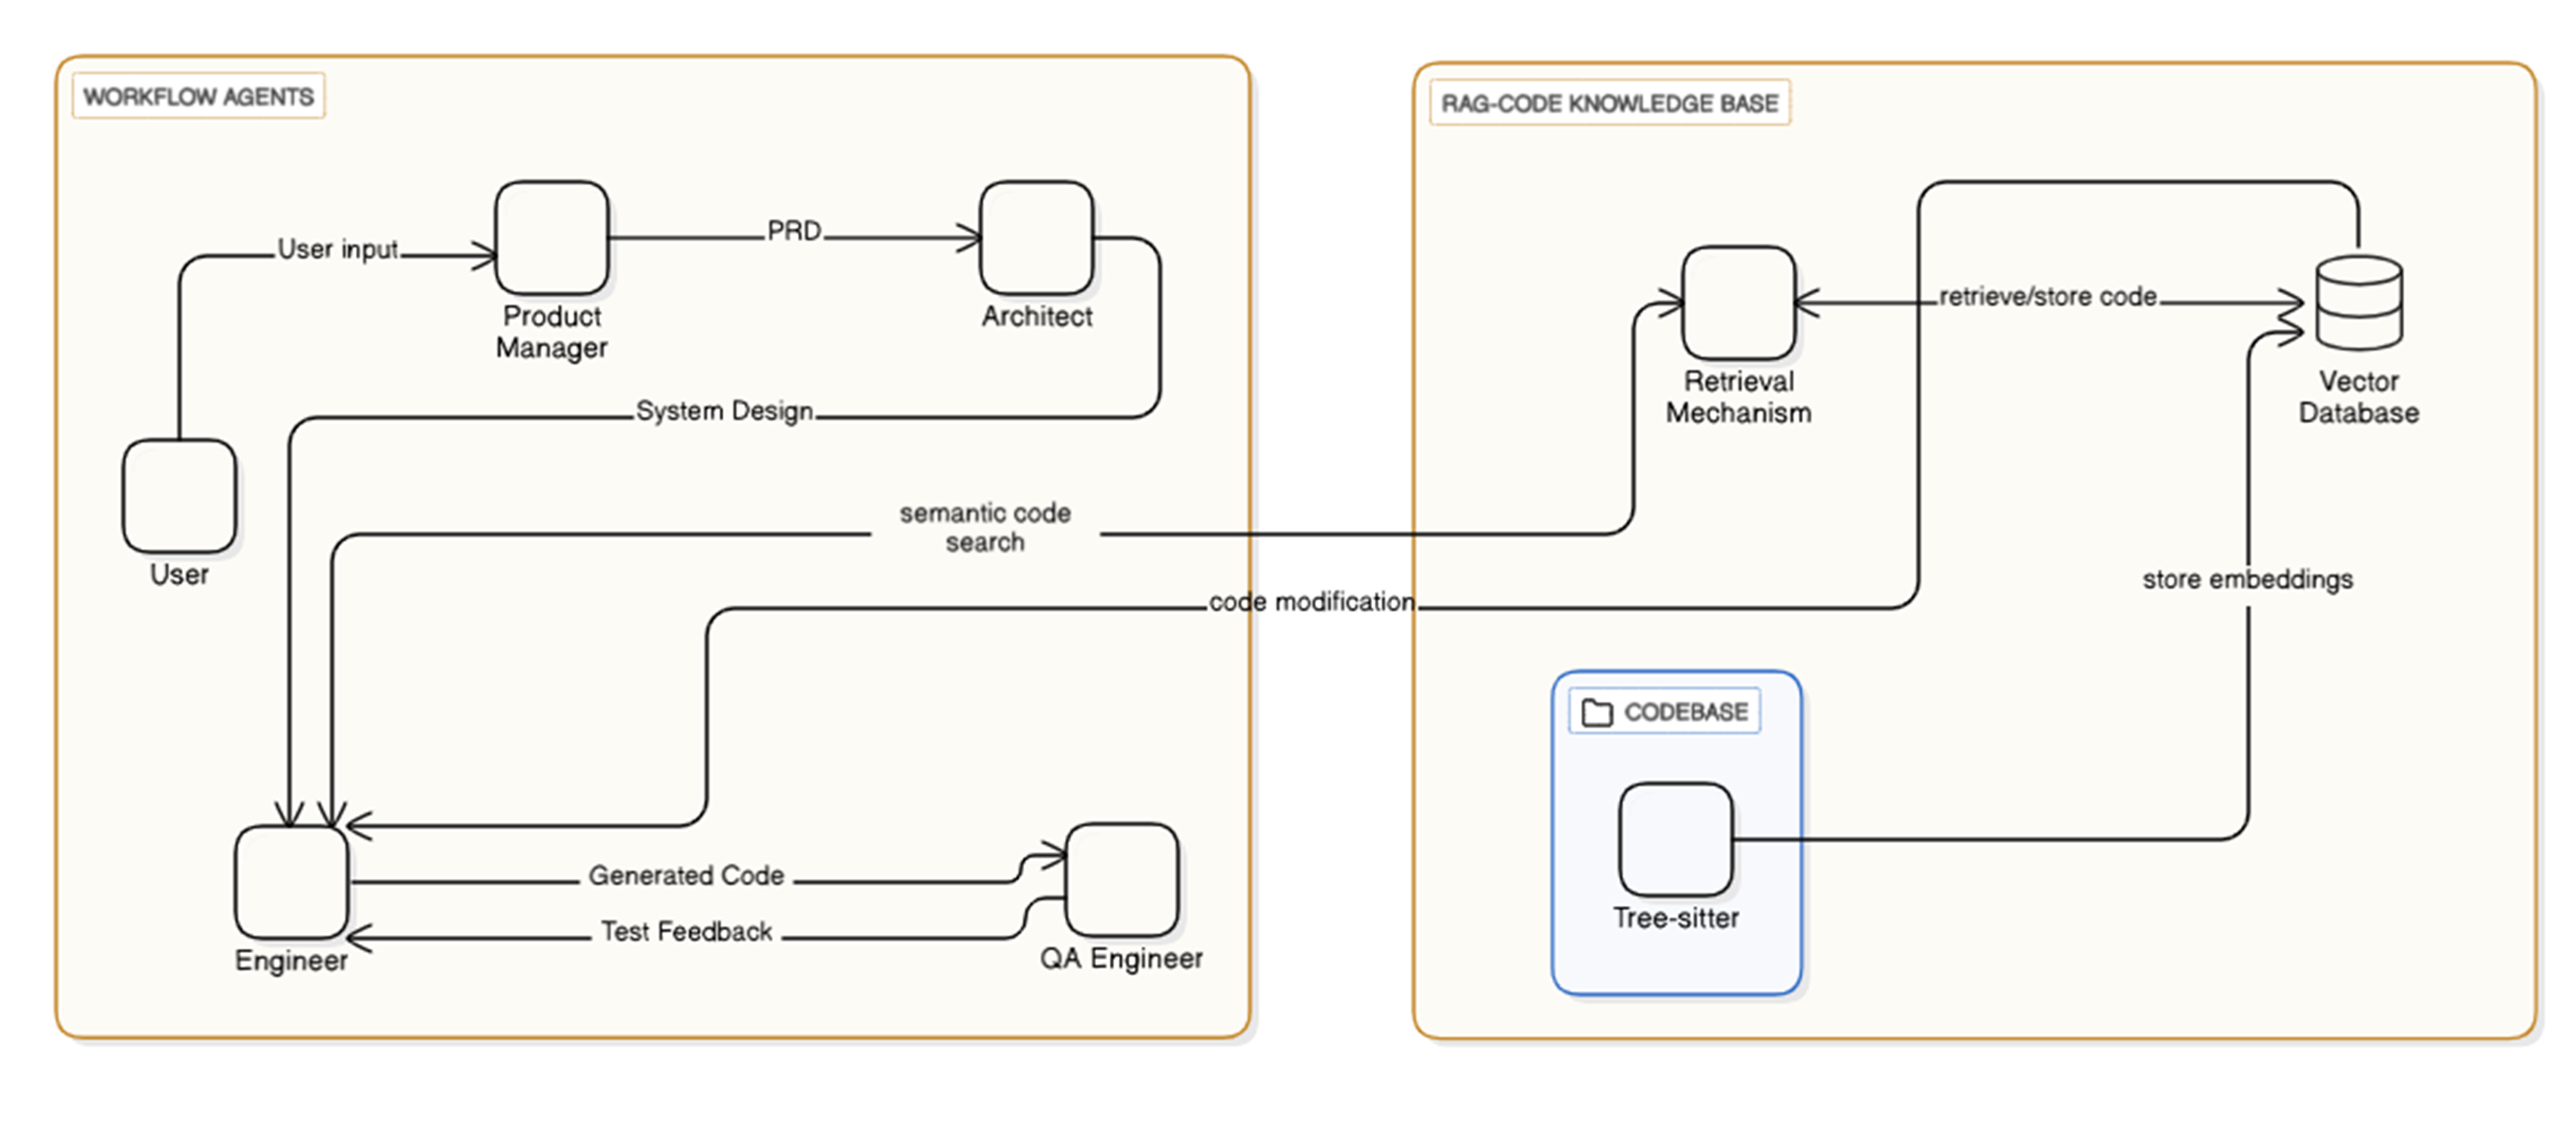
\includegraphics[width=0.9\textwidth]{images/arch.png}
    \caption{High-Level MetaGPT System Architecture}
    \label{fig:architecture}
\end{figure}

The architecture diagram in Figure~\ref{fig:architecture} illustrates the following key components:

\begin{itemize}
    \item \textbf{Frontend Layer:} React-based user interface providing agent management, workflow visualization, and real-time collaboration monitoring.
    \item \textbf{API Gateway:} FastAPI backend serving as the central orchestration point for all agent interactions and workflow management.
    \item \textbf{Agent Framework:} LangGraph-based state graph providing deterministic agent orchestration, with LangChain used as the LLM abstraction layer for calling Google Gemini.
    \item \textbf{Specialized Agents:} Manager, Architect, Engineer, and QA agents with distinct roles and responsibilities.
    \item \textbf{RAG System:} Vector database integration with semantic search capabilities for context-aware code generation and knowledge retrieval.
    \item \textbf{AI Integration:} Gemini API integration providing state-of-the-art language model capabilities for agent reasoning and code generation.
    \item \textbf{Communication Layer:} Shared-state passing via a pipeline service, where each agent reads typed outputs from the previous agent and writes its own output into the same state object.
\end{itemize}


\subsection{Use Case Diagram}

The Use Case diagram illustrates the interactions between the primary actors (User and Multi-Agent System) and the MetaGPT framework, showing the complete software development lifecycle from user input to final code delivery.

\begin{figure}[H]
    \centering
    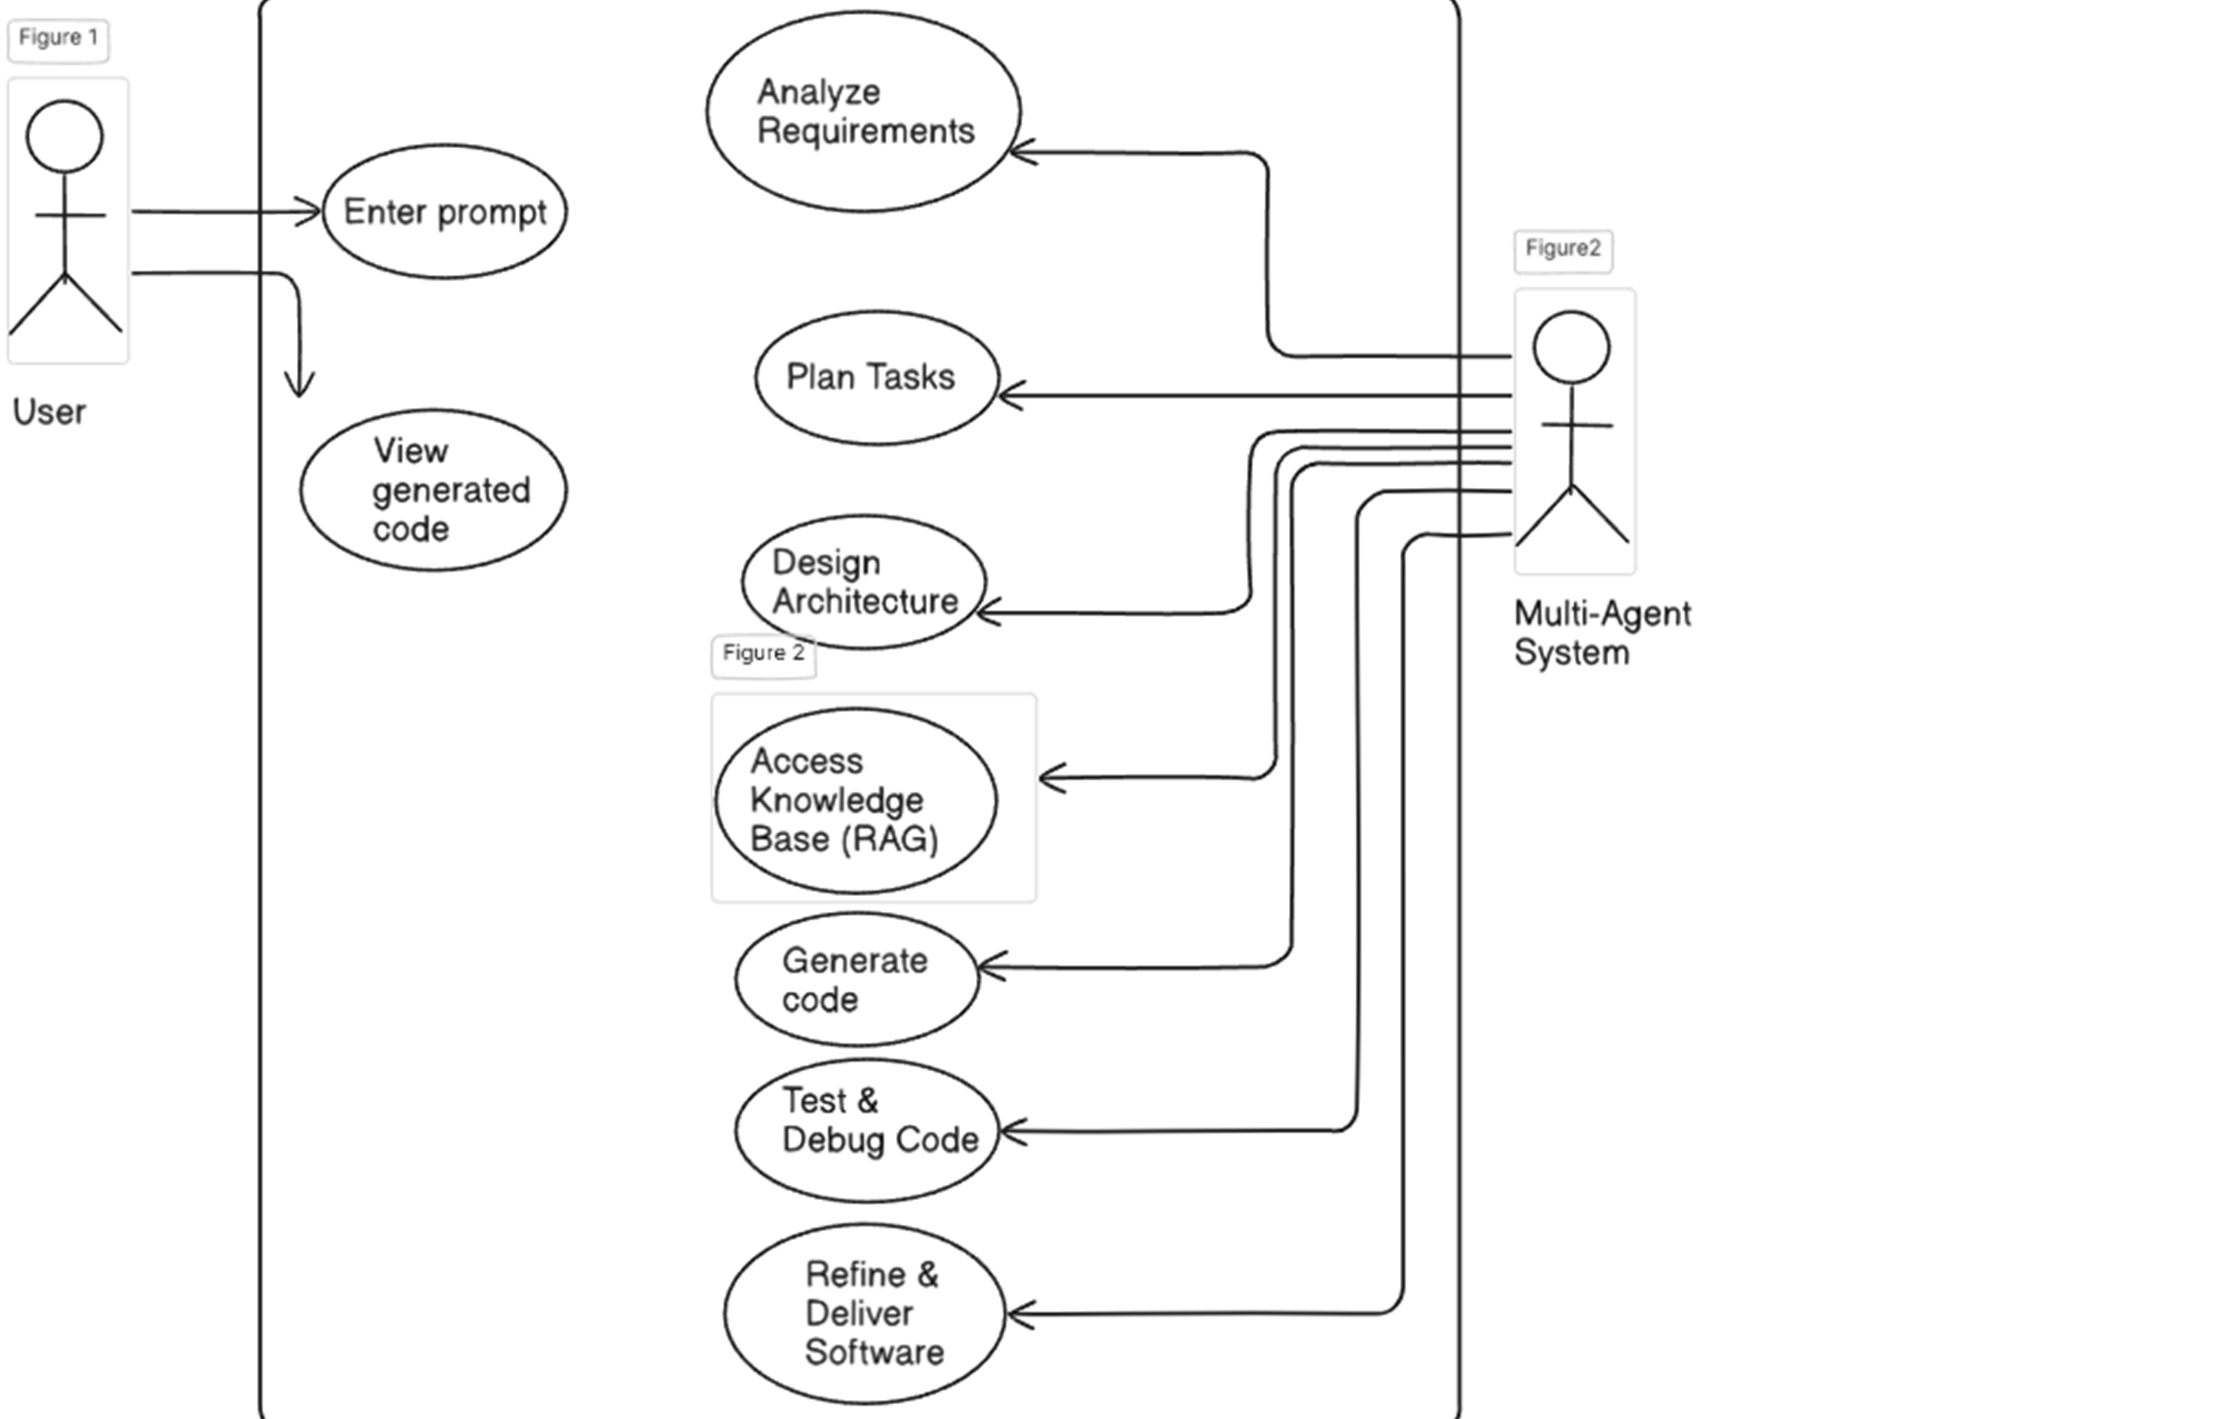
\includegraphics[width=0.8\textwidth]{images/use_case_diagram.png}
    \caption{MetaGPT System Use Case Diagram}
    \label{fig:use_case}
\end{figure}


\section{Detailed Design}
\subsection{Module 1: Backend API Layer}

The first major module is the \textbf{Backend API Layer}, implemented using FastAPI under the \texttt{backend/\allowbreak{}app} package. Its primary responsibility is to expose a stable HTTP interface for all core operations, including project management, pipeline execution, file access, chat-based iteration, and retrieval-augmented generation.

The entry point \texttt{main.py} constructs the FastAPI application, configures middleware, and includes the top-level router defined in \texttt{api/\allowbreak{}router.py}. The router aggregates versioned endpoints under the \texttt{/\allowbreak{}api/\allowbreak{}v1} prefix, delegating to individual endpoint modules such as:
\begin{itemize}
    \item \texttt{api/\allowbreak{}endpoints/\allowbreak{}projects.py} for creating, listing, and retrieving projects.
    \item \texttt{api/\allowbreak{}endpoints/\allowbreak{}pipeline.py} for running the agentic pipeline in batch or streaming mode.
    \item \texttt{api/\allowbreak{}endpoints/\allowbreak{}files.py} for browsing the project file tree and fetching or updating file contents.
    \item \texttt{api/\allowbreak{}endpoints/\allowbreak{}chat.py} for handling iterative chat interactions tied to a project.
    \item \texttt{api/\allowbreak{}endpoints/\allowbreak{}rag.py} and \texttt{api/\allowbreak{}endpoints/\allowbreak{}sandbox.py} for RAG and sandbox-related operations.
\end{itemize}

Each endpoint module validates incoming requests using Pydantic schemas from the \texttt{schemas} package, calls into dedicated service functions, and returns structured responses. Authentication and authorization concerns are centralized in \texttt{auth.py} and integrated into endpoint dependencies where required.

In addition to the core project/pipeline/files/chat endpoints, MetaGPT implements sandbox management endpoints in \texttt{api/\allowbreak{}endpoints/\allowbreak{}sandbox.py} to support live previews of generated projects. The sandbox workflow is intentionally non-blocking: the \texttt{/\allowbreak{}{project\_\allowbreak{}id}/create} endpoint returns \textbf{202 Accepted} immediately and triggers sandbox creation as a background task, while clients poll \texttt{/\allowbreak{}{project\_\allowbreak{}id}/status} until the sandbox becomes \texttt{ready} and a \texttt{preview\_\allowbreak{}url} is available. This design prevents request timeouts during dependency installation and dev-server startup.

\subsection{Module 2: Agent Orchestration and Graph}

The second module is the \textbf{Agent Orchestration and Graph Module}, which coordinates the sequence of Manager, Architect, Engineer, and QA agents using LangGraph. The overall pipeline state is defined in \texttt{graph/\allowbreak{}state.py}, where a central data structure captures the prompt, intermediate artifacts, agent outputs, and final project representation.

The orchestration logic in \texttt{graph/\allowbreak{}orchestrator.py} builds a directed graph whose nodes correspond to individual agents and whose edges represent valid transitions. For example, the Manager node takes a raw user prompt and produces a structured requirement specification, which becomes input to the Architect node. The Architect node generates a high-level system design and file plan, which is passed to the Engineer node to create concrete source files. Finally, the QA node inspects the generated artifacts, produces test cases, and records quality-related feedback.

The orchestrator integrates with LangChain’s LLM abstractions to call Google Gemini via helper functions defined in the \texttt{llm} module. It also records intermediate outputs so that the frontend can display an execution timeline and visualizations of agent reasoning. Error handling, retries, and logging are centralized here, making the pipeline robust and easier to debug or extend with additional agents in the future.

\subsection{Module 3: Storage and Project Management}

The third module is the \textbf{Storage and Project Management Module}, which persists all artifacts produced by the pipeline and exposes higher-level operations for managing projects. This module is implemented primarily in the \texttt{storage} and \texttt{models} packages.

Domain models such as \texttt{models/\allowbreak{}project.py} and \texttt{models/\allowbreak{}user.py} describe core entities, while storage backends in \texttt{storage/\allowbreak{}project\_\allowbreak{}store.py} and \texttt{storage/\allowbreak{}file\_\allowbreak{}store.py} handle reading and writing data. Project state is persisted in \textbf{MongoDB} using the Beanie ODM (with Motor as the async driver), as implemented in \texttt{db.py}, \texttt{models/\allowbreak{}project.py}, and \texttt{storage/\allowbreak{}project\_\allowbreak{}store.py}. The project store is responsible for:
\begin{itemize}
    \item Creating a new project directory structure in a configurable \texttt{PROJECTS\_\allowbreak{}DIR} for generated code files.
    \item Recording metadata such as project identifiers, associated prompts, and timestamps in MongoDB.
    \item Listing existing projects and resolving paths for files within a given project.
\end{itemize}

The file store provides operations to:
\begin{itemize}
    \item Generate a tree representation of project files for the frontend file explorer.
    \item Read file contents for display in the code viewer.
    \item Apply updates to files when users edit code through the interface.
\end{itemize}

Together, these components decouple persistent storage concerns from the agent pipeline and API layer. This persistence layer stores project metadata, pipeline status, and agent outputs (including generated files), enabling recovery after server restarts and supporting long-running workflows. When ephemeral disk cache is missing, the pipeline service can restore project files from MongoDB back to disk so that file browsing and preview remain functional.

\subsection{Module 4: Frontend User Interface}

The fourth module is the \textbf{Frontend User Interface}, implemented with Next.js, TypeScript, and Tailwind CSS under the \texttt{frontend/\allowbreak{}src} directory. It provides an interactive, dark-themed workspace where users can manage projects and visualize the behavior of the agent pipeline.

The App Router structure in \texttt{src/\allowbreak{}app} defines key pages:
\begin{itemize}
    \item \texttt{page.tsx} as the landing page for entering prompts and viewing recent projects.
    \item \texttt{projects/\allowbreak{}page.tsx} for listing all projects retrieved from the backend.
    \item \texttt{project/\allowbreak{}[id]/\allowbreak{}page.tsx} as the main workspace for a specific project, showing files, agent outputs, and chat.
    \item \texttt{signin/\allowbreak{}page.tsx} and \texttt{signup/\allowbreak{}page.tsx} for authentication flows (if enabled).
\end{itemize}

Reusable components in \texttt{src/\allowbreak{}components} encapsulate major UI features:
\begin{itemize}
    \item \texttt{FileExplorer.tsx} renders the project tree and allows users to select files.
    \item \texttt{CodeViewer.tsx} displays syntax-highlighted source code and possibly supports editing.
    \item \texttt{AgentOutputs.tsx} shows structured reasoning and outputs from each agent in the pipeline.
    \item \texttt{ExecutionTimeline.tsx} visualizes the sequence and status of agent executions.
    \item \texttt{ChatPanel.tsx} enables iterative conversations tied to a particular project.
\end{itemize}

Client-side state is managed using stores defined in \texttt{src/\allowbreak{}lib/\allowbreak{}store.ts} and related files, while API communication is abstracted in \texttt{src/\allowbreak{}lib/\allowbreak{}api.ts}. Global styles and Tailwind configuration ensure a consistent look-and-feel across the application.

\subsection{Module 5: LLM, SOP, and Retrieval}

The fifth module is the \textbf{LLM, SOP, and Retrieval Module}, which encapsulates all logic related to configuring the underlying LLM, defining agent SOPs, and supporting retrieval-augmented generation (RAG). This module ties together the conceptual behavior of agents with concrete model calls and knowledge sources.

The \texttt{llm/\allowbreak{}gemini.py} file provides helper functions such as \texttt{get\_\allowbreak{}llm} and \texttt{get\_\allowbreak{}llm\_\allowbreak{}with\_\allowbreak{}structured\_\allowbreak{}output}, which create LangChain-compatible LLM instances backed by Google Gemini. Configuration values such as model name, temperature, maximum tokens, and API key are read from \texttt{config.py} and environment variables, ensuring that model behavior can be tuned without changing application code.

Agent behaviors are specified in \texttt{sop/\allowbreak{}definitions.py}, where each agent’s role, objectives, inputs, outputs, constraints, and quality checklist are documented. These SOPs are consumed by the agent implementations in the \texttt{agents} package, providing a clear contract between high-level design and concrete prompts issued to the LLM.

The RAG submodule in \texttt{rag} contains utilities for indexing and retrieving relevant documents. Files such as \texttt{rag/\allowbreak{}indexer.py}, \texttt{rag/\allowbreak{}vector\_\allowbreak{}store.py}, \texttt{rag/\allowbreak{}retriever.py}, and \texttt{rag/\allowbreak{}embeddings.py} manage the creation of vector embeddings, storage of vectors, and retrieval of context for augmenting LLM prompts. This enables MetaGPT to ground agent reasoning in existing project artifacts or external knowledge bases, improving accuracy and consistency for complex tasks.

\section{Data Flow Diagram}

Data Flow Diagrams (DFDs) illustrate the movement of data within the MetaGPT system and how information flows between different agents and components.

\subsection{Context Diagram (Level 0 DFD)}
The Level 0 DFD illustrates the high-level interaction between the User and the MetaGPT system, showing the complete workflow from user input to final code delivery.

\begin{figure}[H]
    \centering
    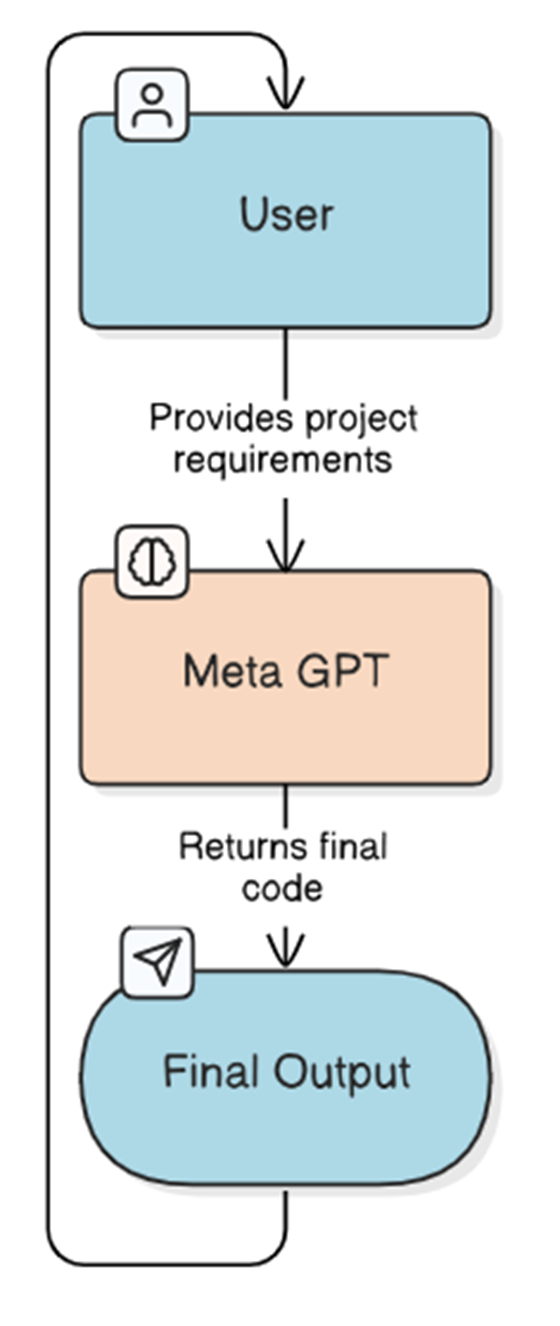
\includegraphics[width=0.3\textwidth]{images/dfd_level_0_final.png}
    \caption{DFD Level 0 - MetaGPT System}
    \label{fig:dfd_0}
\end{figure}

\subsection{Level 1 DFD}
The Level 1 DFD illustrates the internal workings of the MetaGPT system, showing how specialized agents collaborate to transform user requirements into validated code output through structured workflows and iterative feedback loops.

\begin{figure}[H]
    \centering
    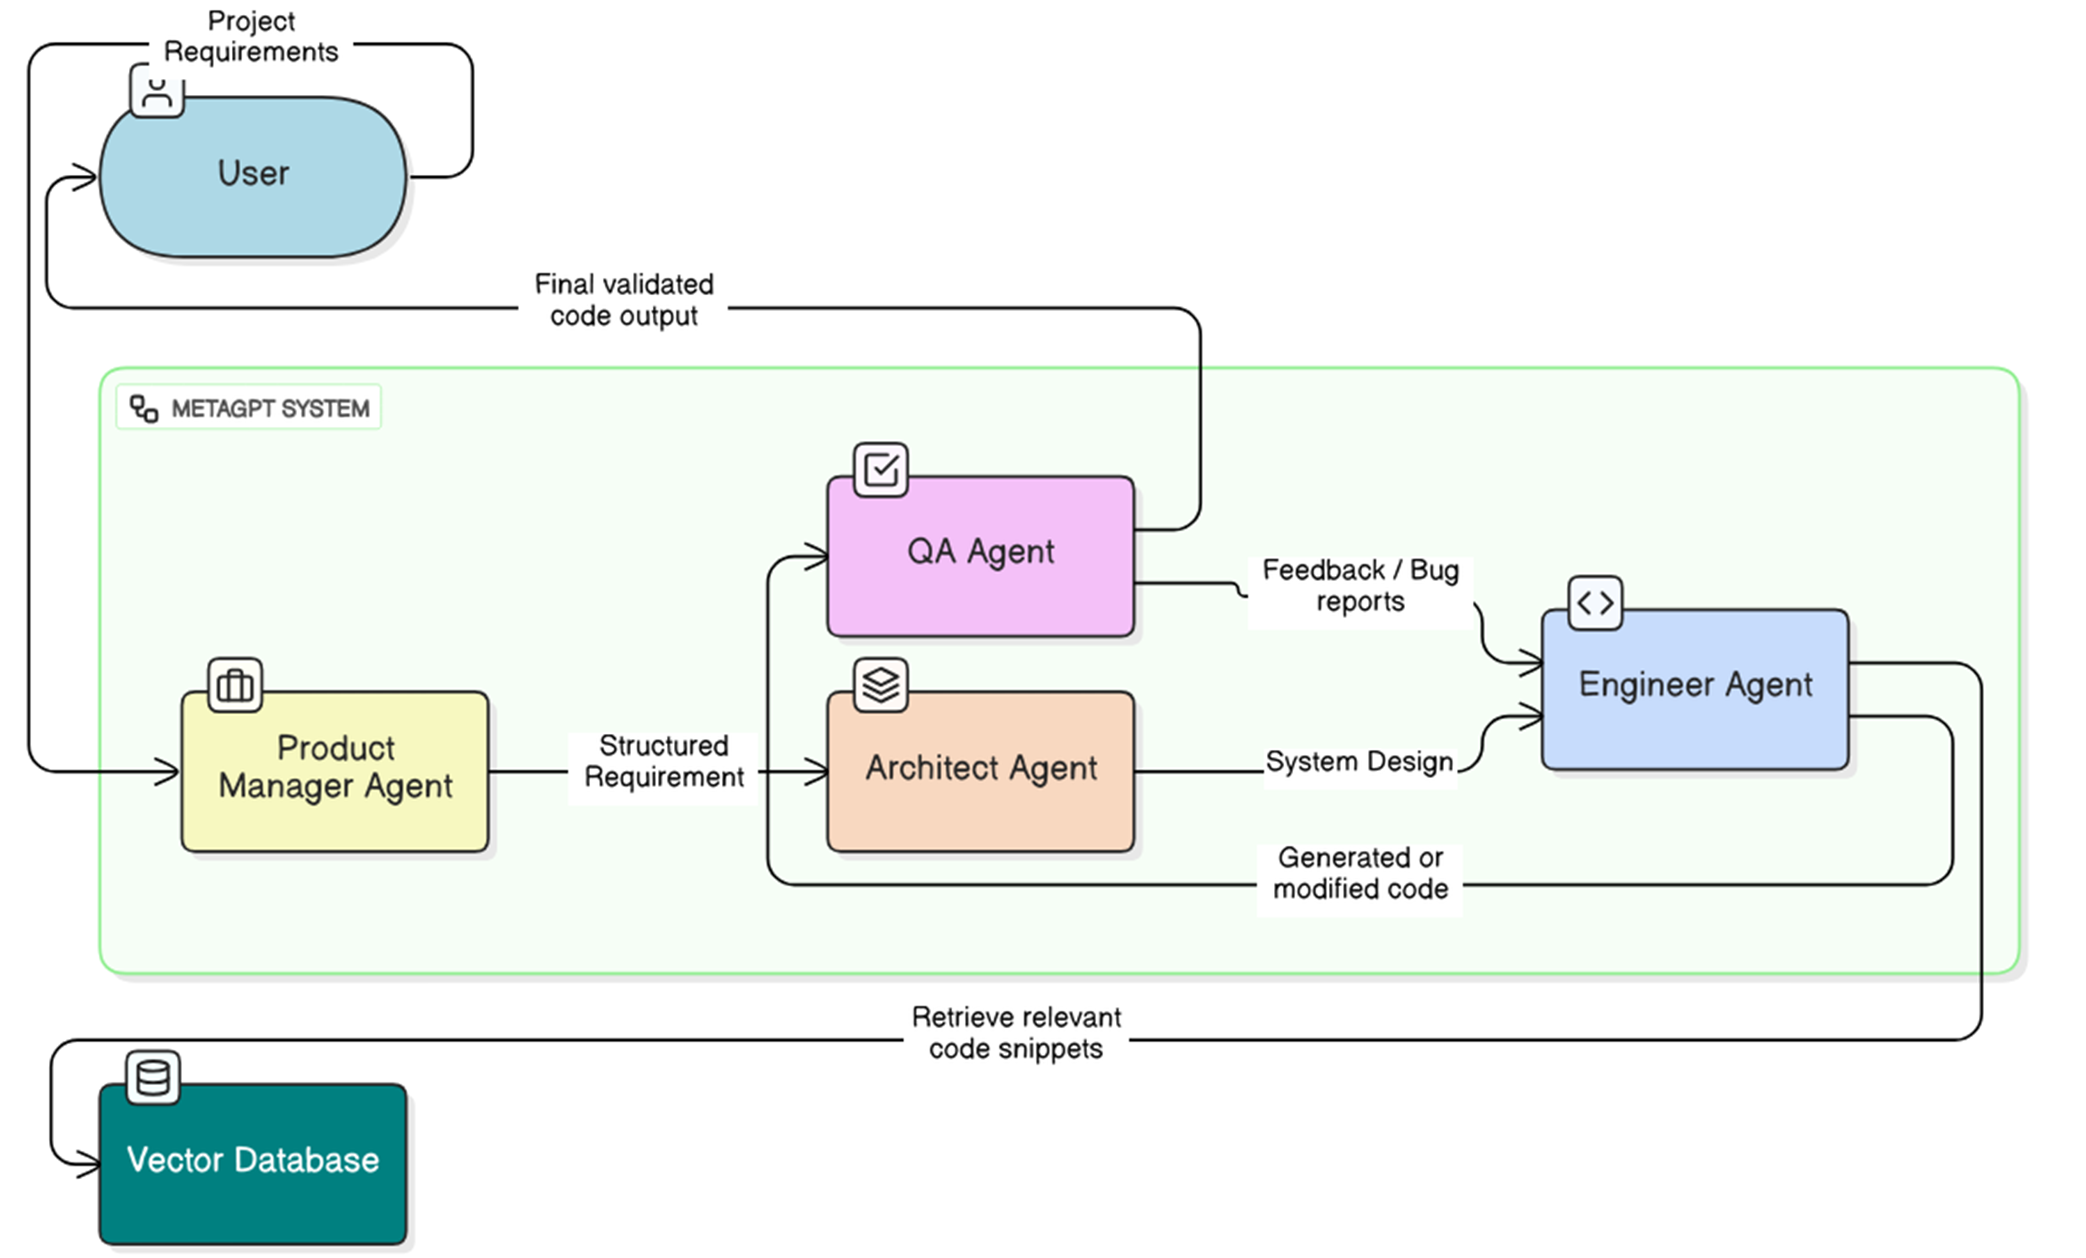
\includegraphics[width=1.0\textwidth]{images/dfd_level_1_final.png}
    \caption{DFD Level 1 - MetaGPT System Internal Workflow}
    \label{fig:dfd_1}
\end{figure}

\subsection{Level 2 DFD}

The Level 2 Data Flow Diagram provides a detailed decomposition of the MetaGPT system's internal agent collaboration process, showing the granular data flows and transformations that occur within each agent's specialized workflow.

\begin{figure}[H]
    \centering
    \makebox[\textwidth]{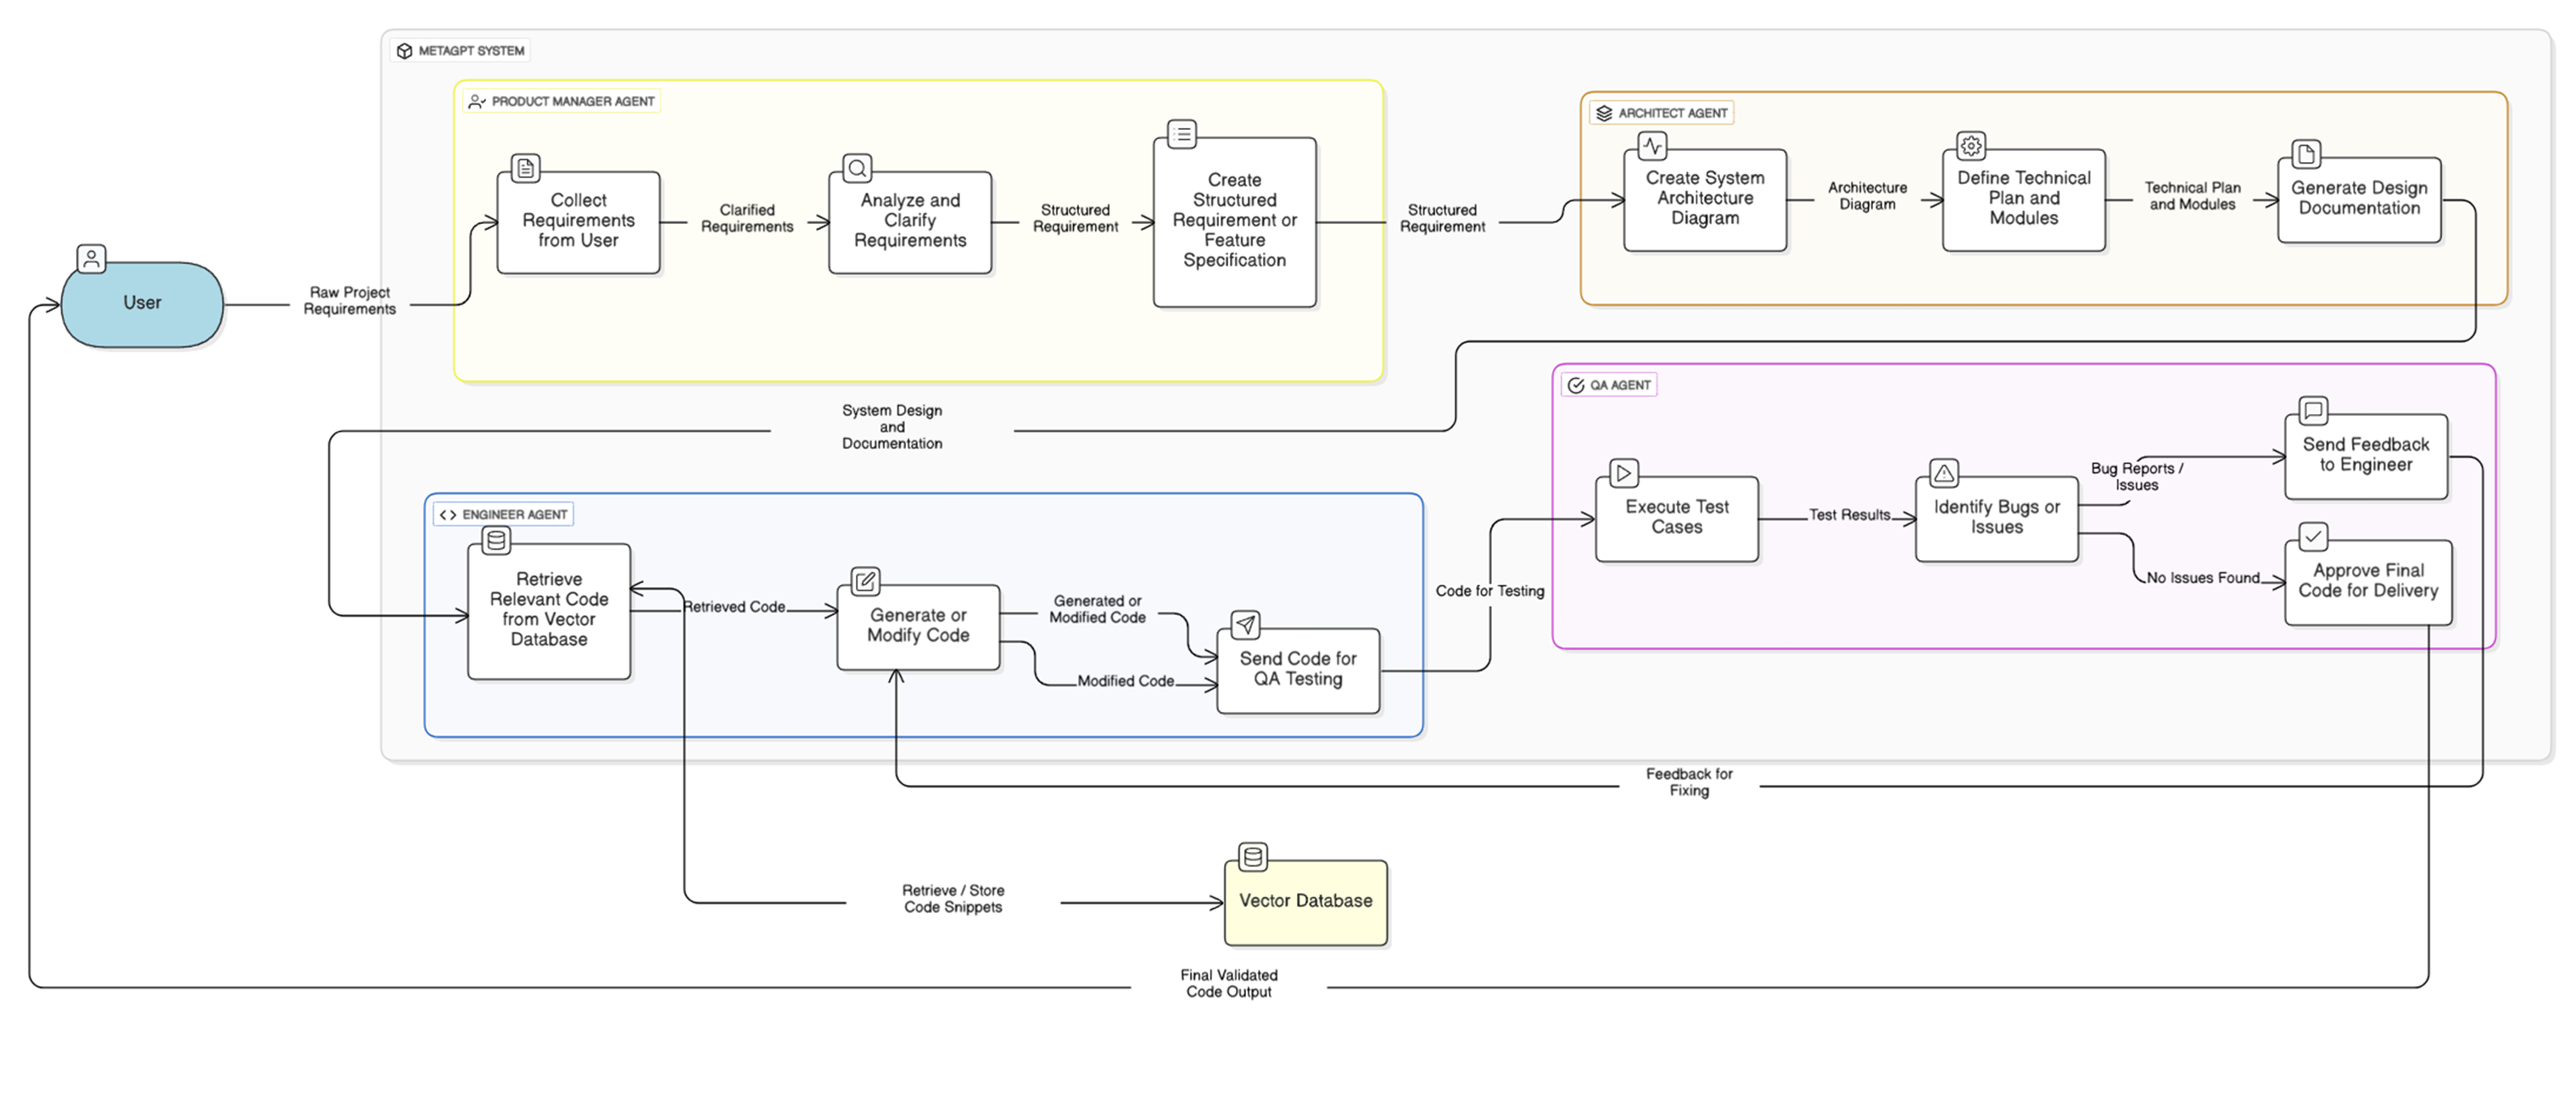
\includegraphics[width=\paperwidth]{images/dfd2.png}}
    \caption{DFD Level 2 — Detailed Agent Collaboration Process}
    \label{fig:dfd_2}
\end{figure}

\section{ER Diagram}

Lorem ipsum dolor sit amet, consectetur adipiscing elit. 
Sed do eiusmod tempor incididunt ut labore et dolore magna aliqua. 
Ut enim ad minim veniam, quis nostrud exercitation ullamco laboris nisi ut aliquip ex ea commodo consequat. 
Duis aute irure dolor in reprehenderit in voluptate velit esse cillum dolore eu fugiat nulla pariatur. 
Excepteur sint occaecat cupidatat non proident, sunt in culpa qui officia deserunt mollit anim id est laborum.

\section{UI Design}

The User Interface (UI) is designed to be clean, modern, and intuitive, prioritizing the agent management and workflow visualization experience. The following screenshots illustrate the key screens of the application.

\begin{figure}[H]
    \centering
    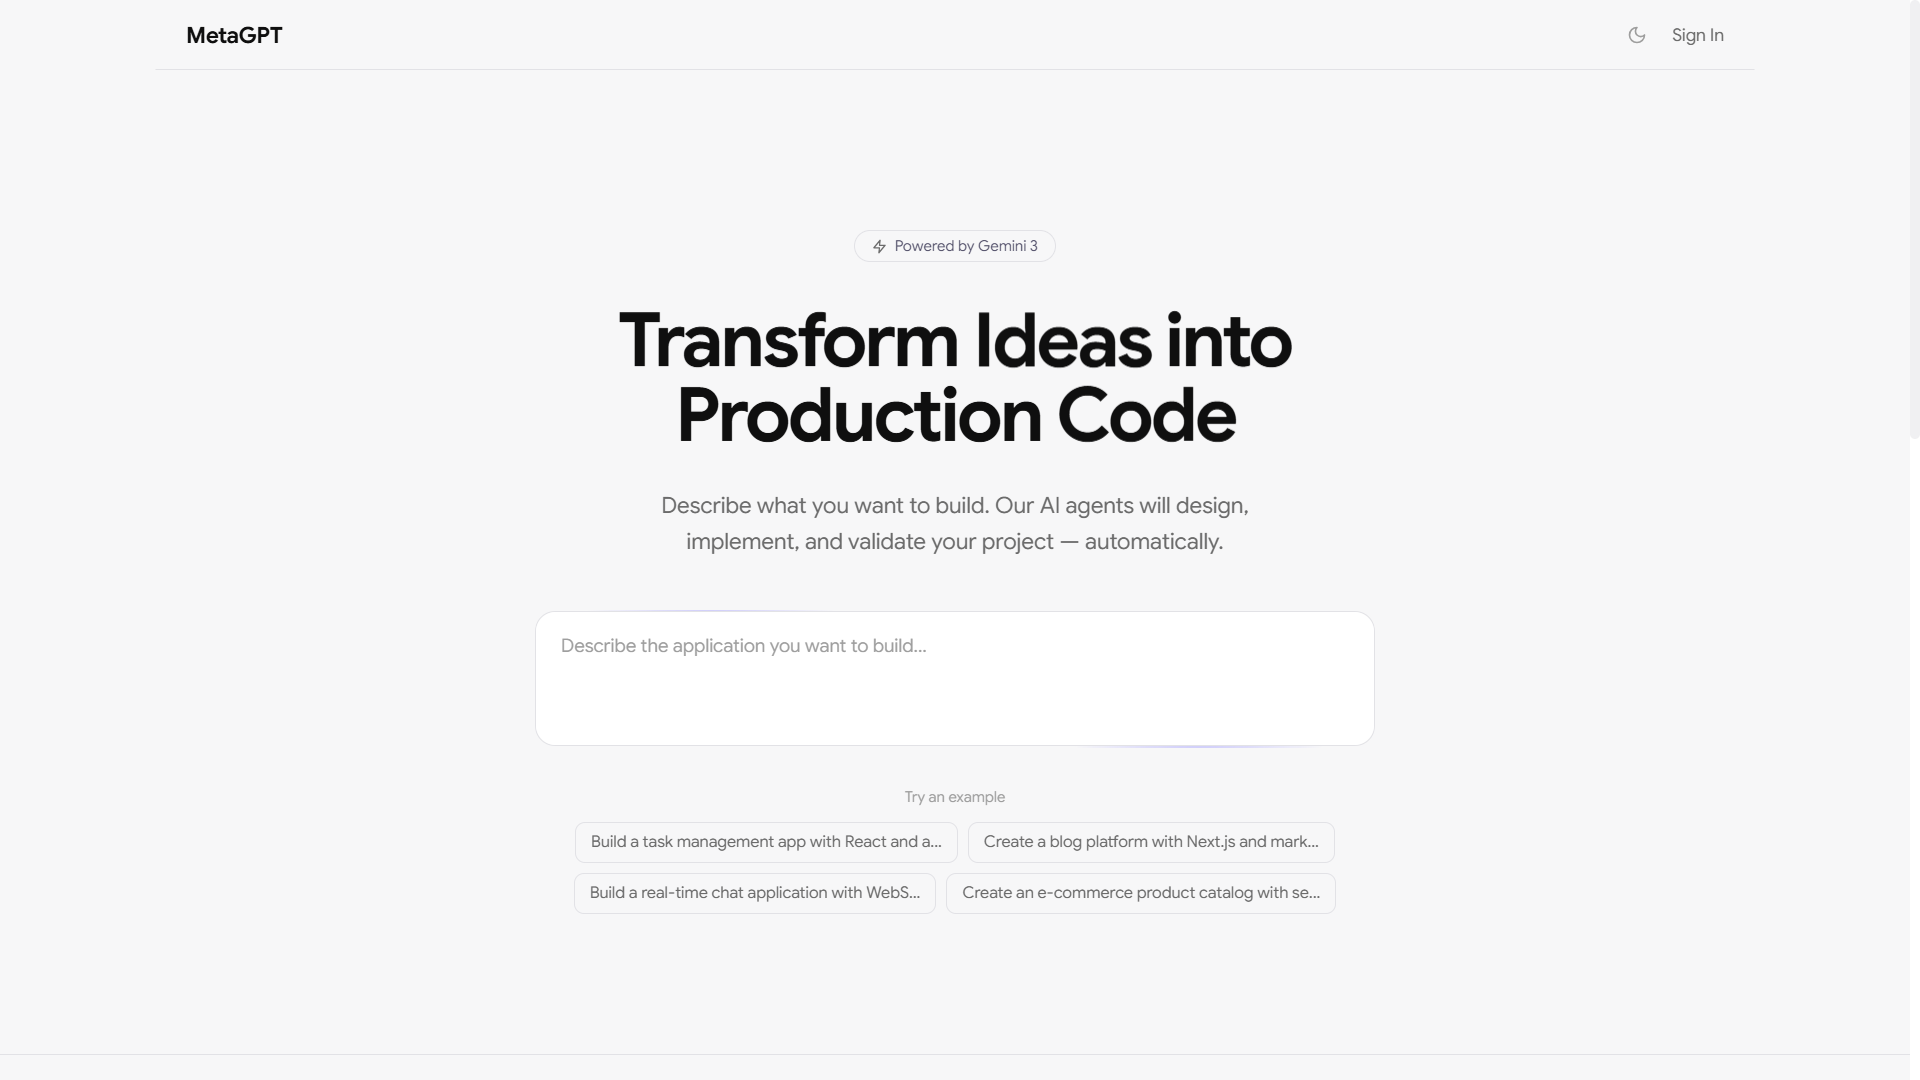
\includegraphics[width=1\textwidth]{images/home_page.png}
    \caption{MetaGPT — Home Page}
    \label{fig:ui_home}
\end{figure}

\vspace{1em}

\begin{figure}[H]
    \centering
    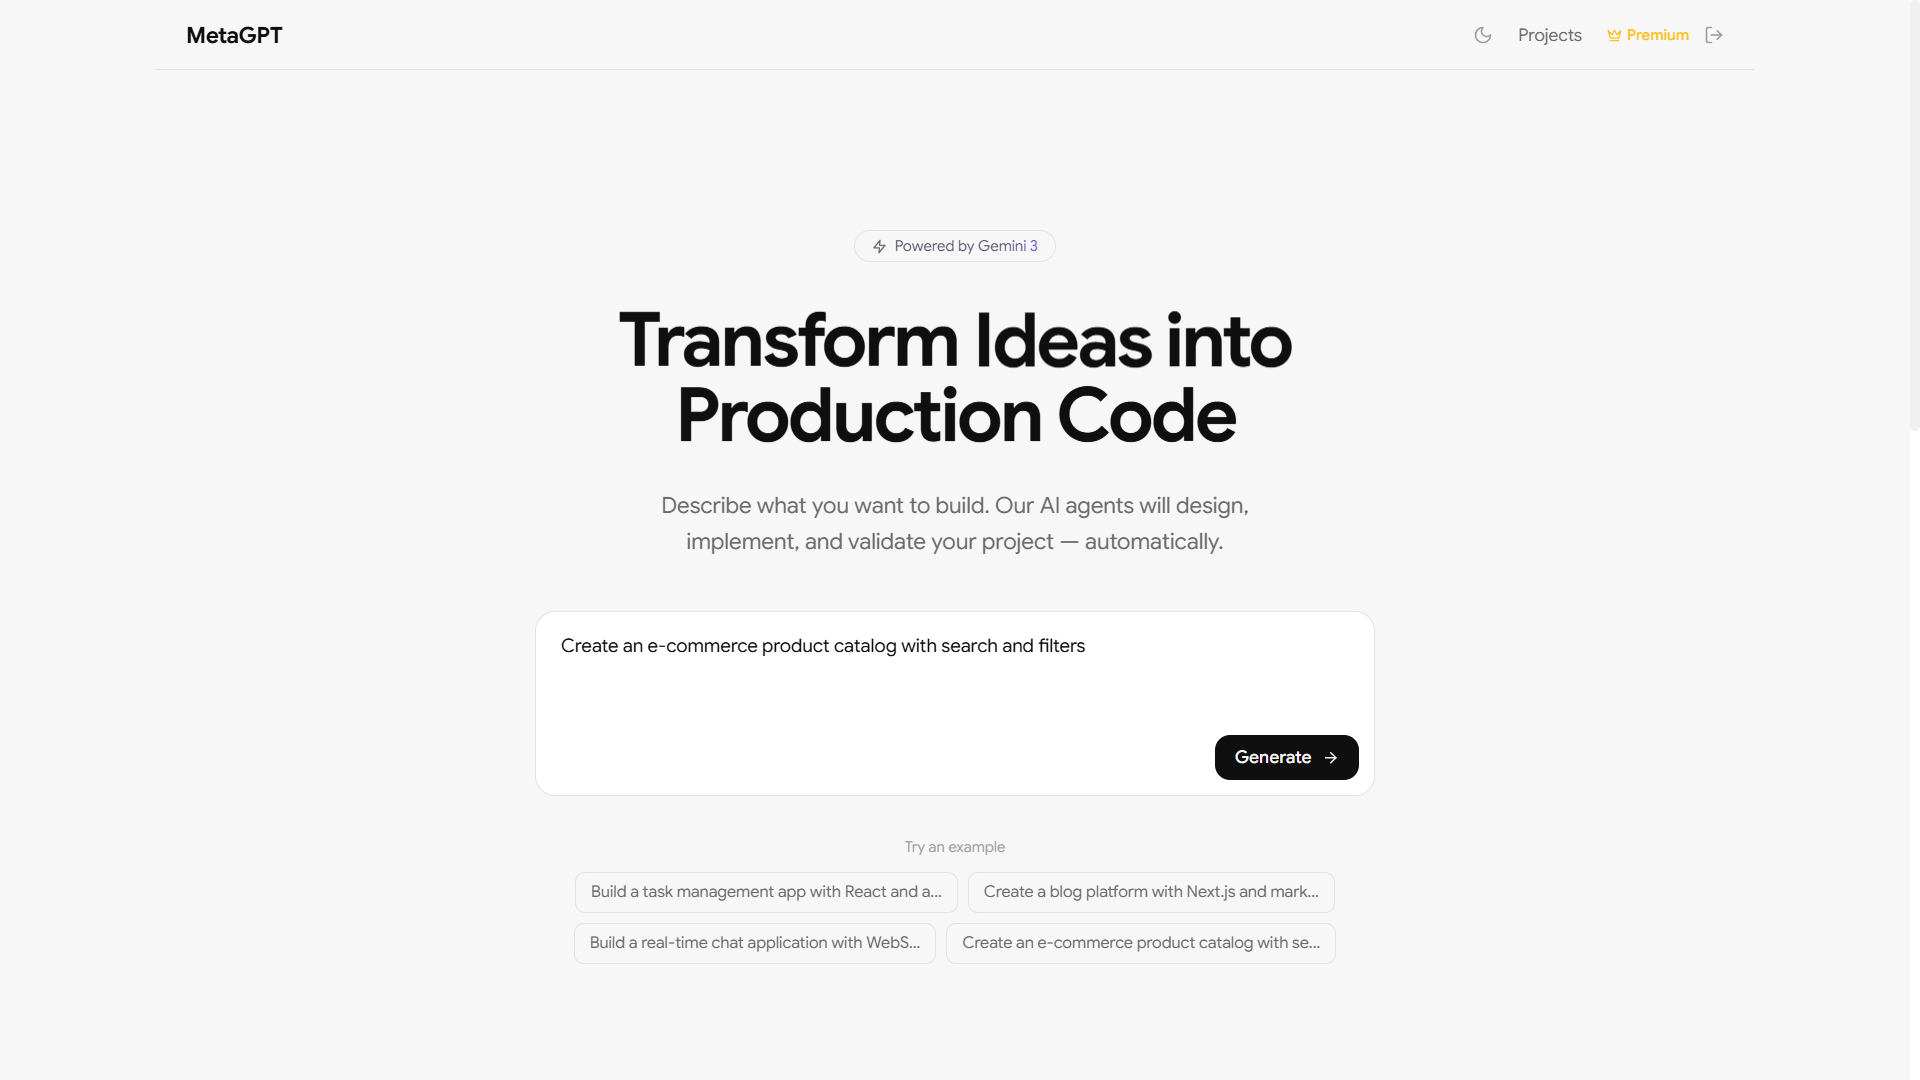
\includegraphics[width=1\textwidth]{images/home_page_with_prompt.png}
    \caption{MetaGPT — Home Page with Prompt Entered}
    \label{fig:ui_home_prompt}
\end{figure}

\vspace{1em}

\begin{figure}[H]
    \centering
    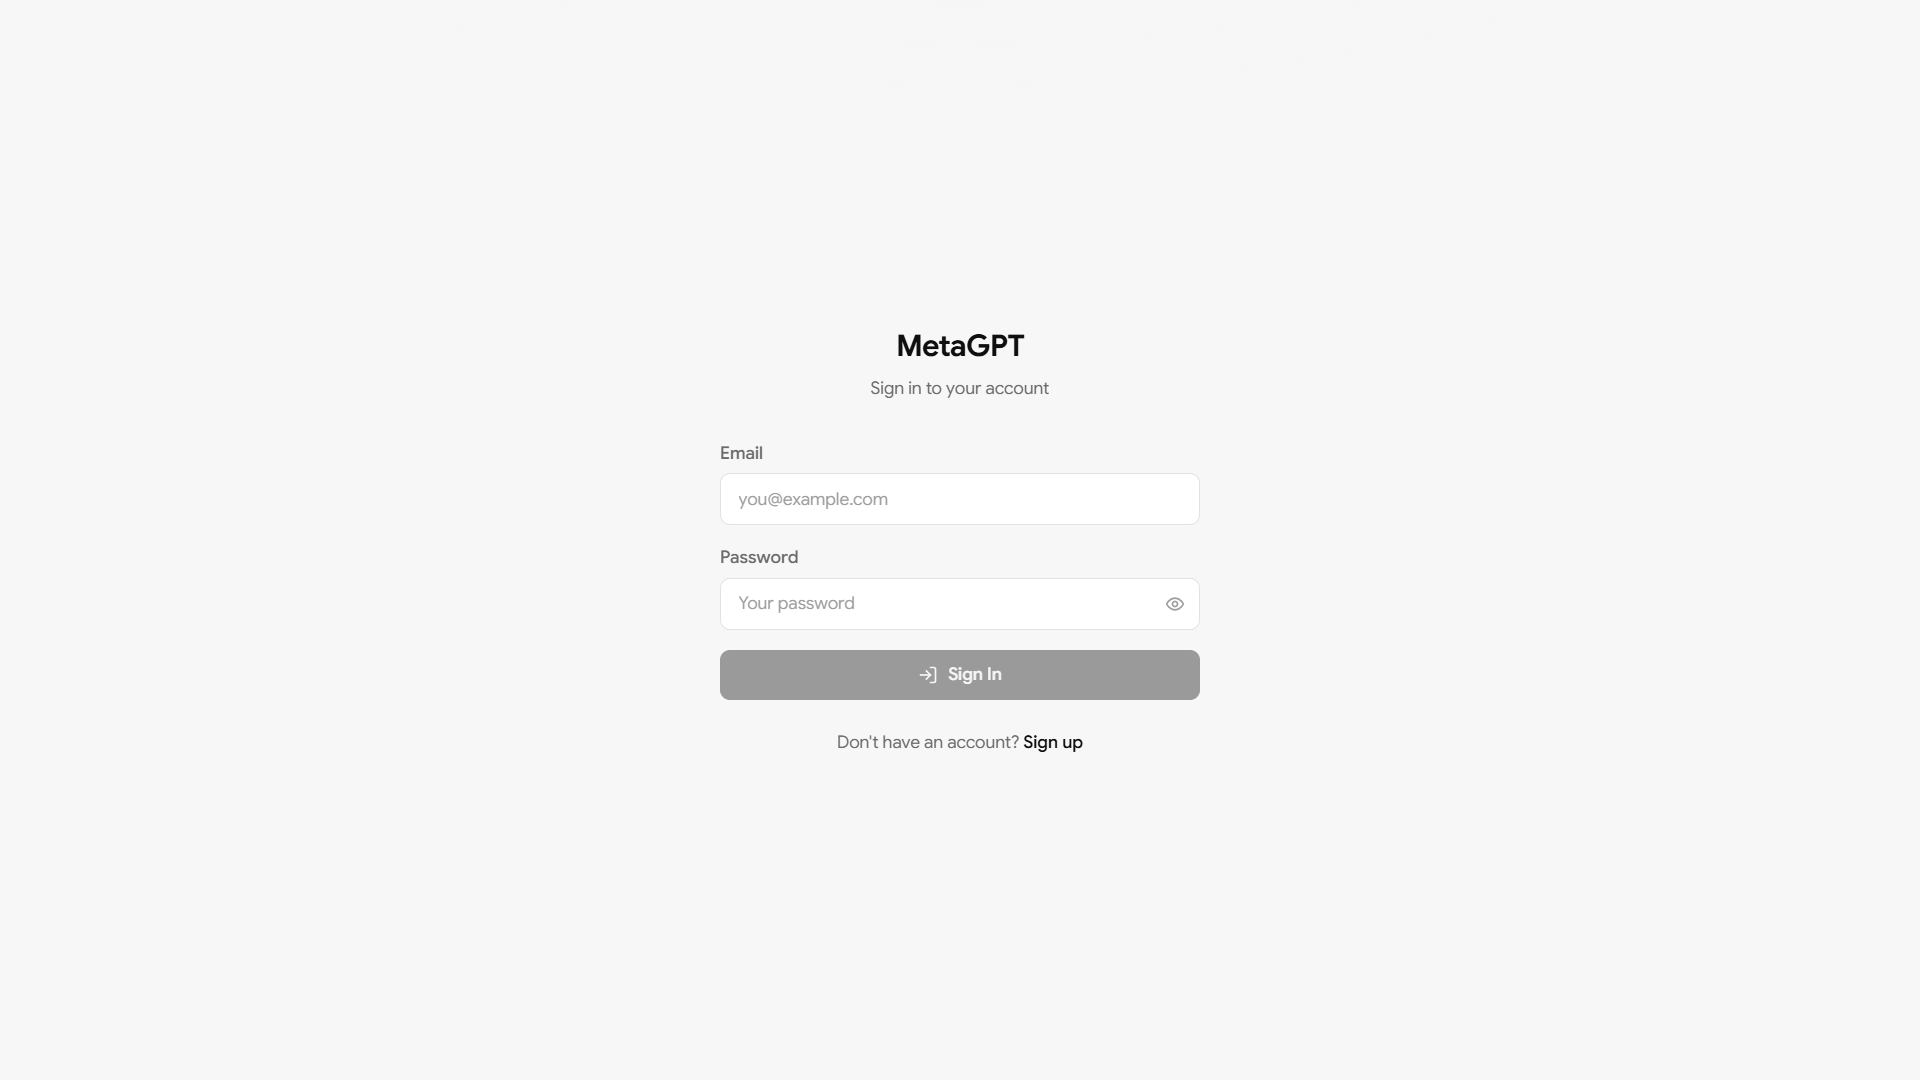
\includegraphics[width=1\textwidth]{images/signin_page.png}
    \caption{MetaGPT — Sign In Page}
    \label{fig:ui_signin}
\end{figure}

\vspace{1em}

\begin{figure}[H]
    \centering
    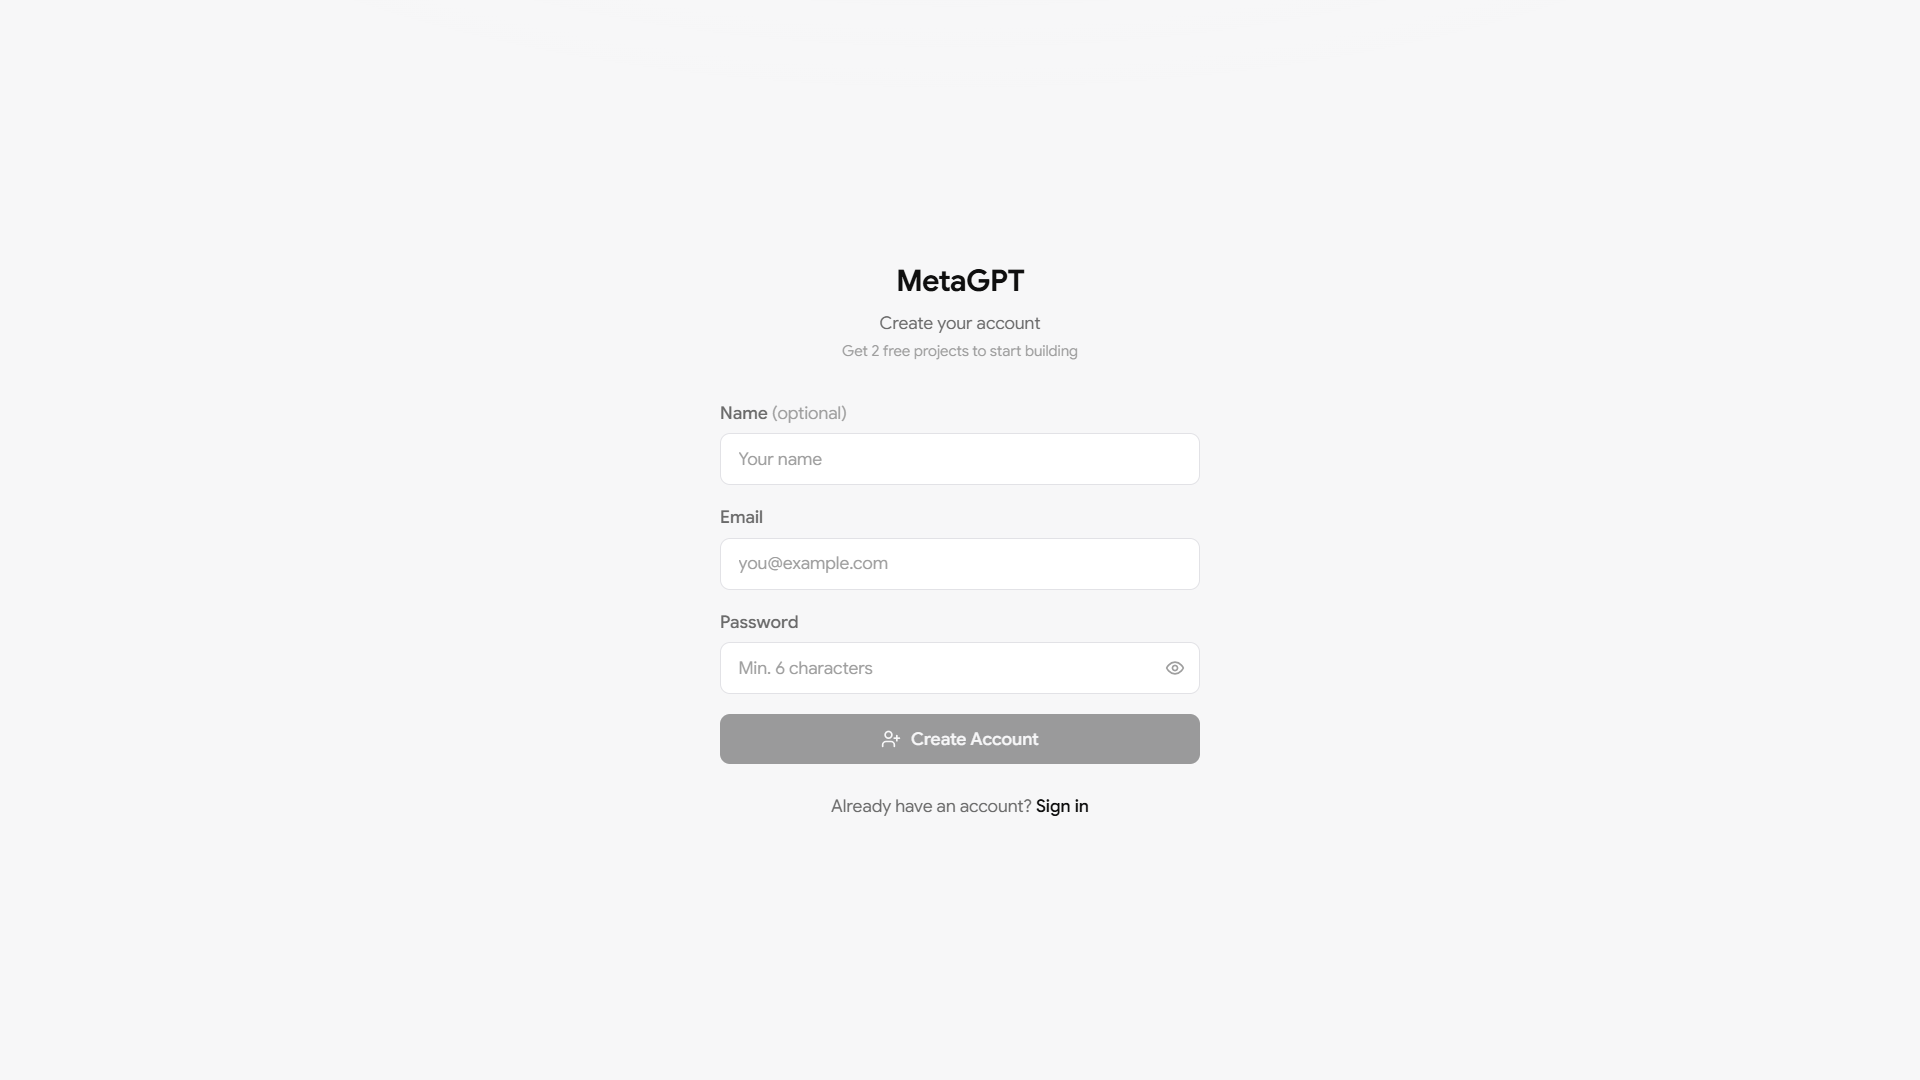
\includegraphics[width=1\textwidth]{images/signup_page.png}
    \caption{MetaGPT — Sign Up Page}
    \label{fig:ui_signup}
\end{figure}

\vspace{1em}

\begin{figure}[H]
    \centering
    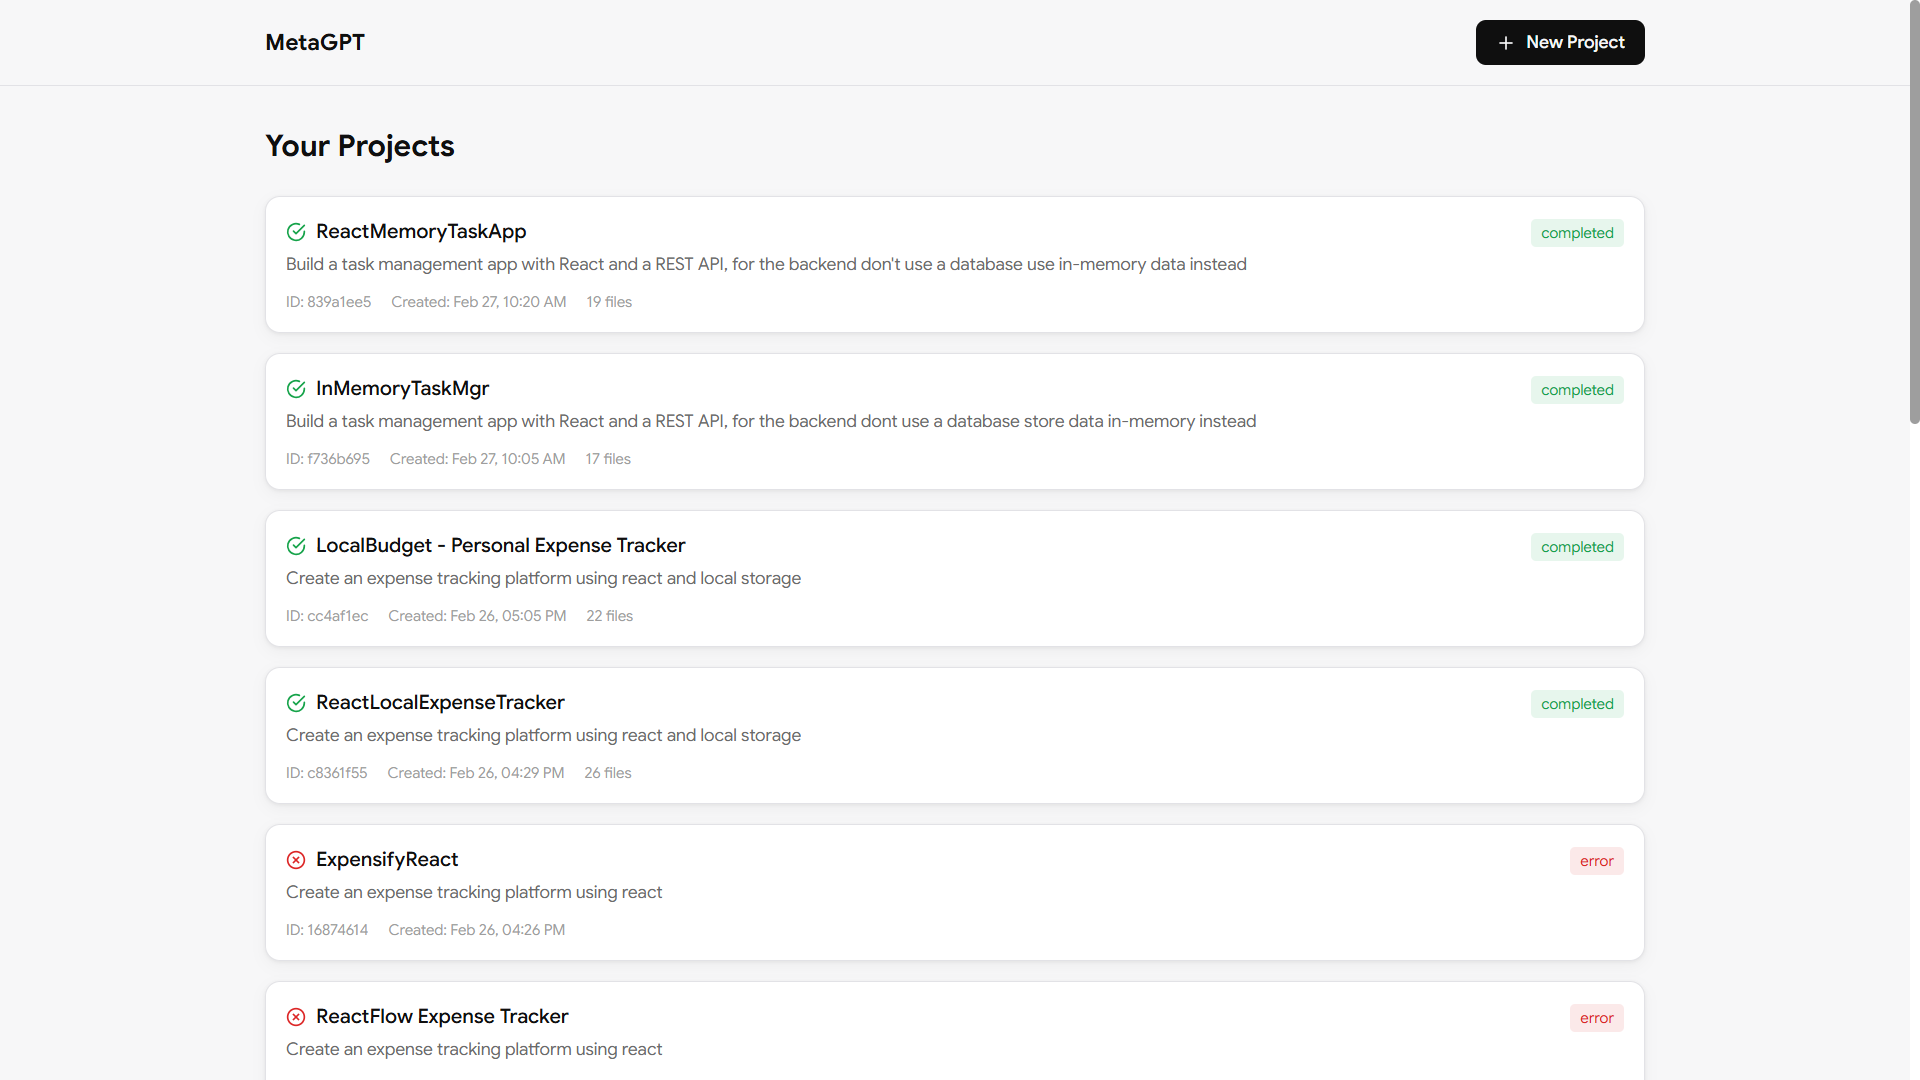
\includegraphics[width=1\textwidth]{images/list_of_projects.png}
    \caption{MetaGPT — List of Projects}
    \label{fig:ui_projects}
\end{figure}

\vspace{1em}

\begin{figure}[H]
    \vspace*{-\intextsep}
    \centering
    \captionsetup{aboveskip=0pt,belowskip=2pt}
    \caption{MetaGPT — Manager Agent Output}
    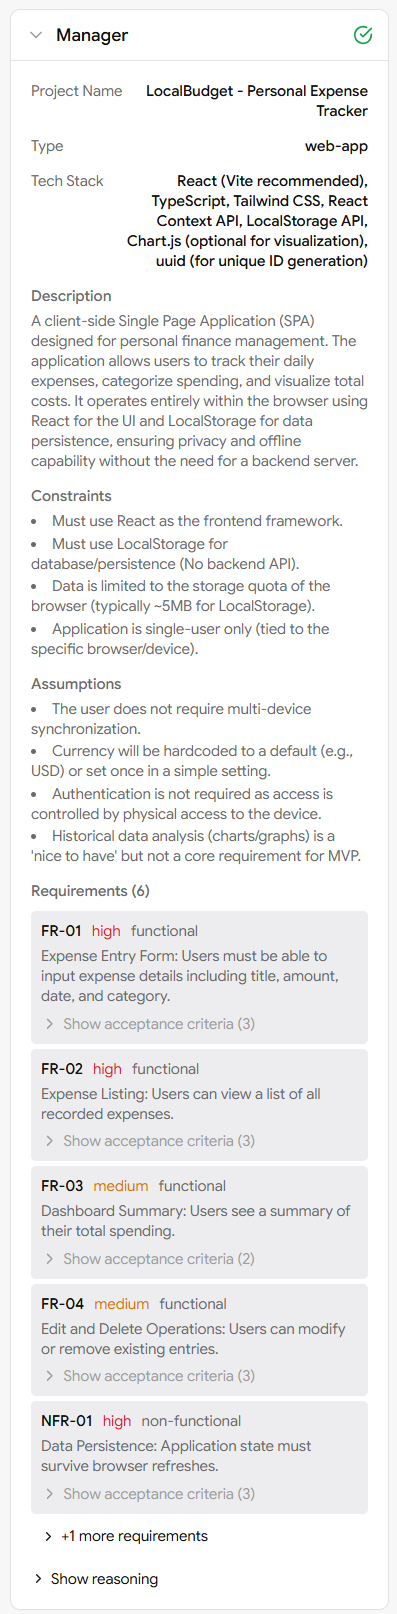
\includegraphics[height=\textheight,keepaspectratio]{images/manager_output.png}
    \label{fig:ui_manager}
\end{figure}

\vspace{1em}

\begin{figure}[H]
    \vspace*{-\intextsep}
    \centering
    \captionsetup{aboveskip=0pt,belowskip=2pt}
    \caption{MetaGPT — Architect Agent Output}
    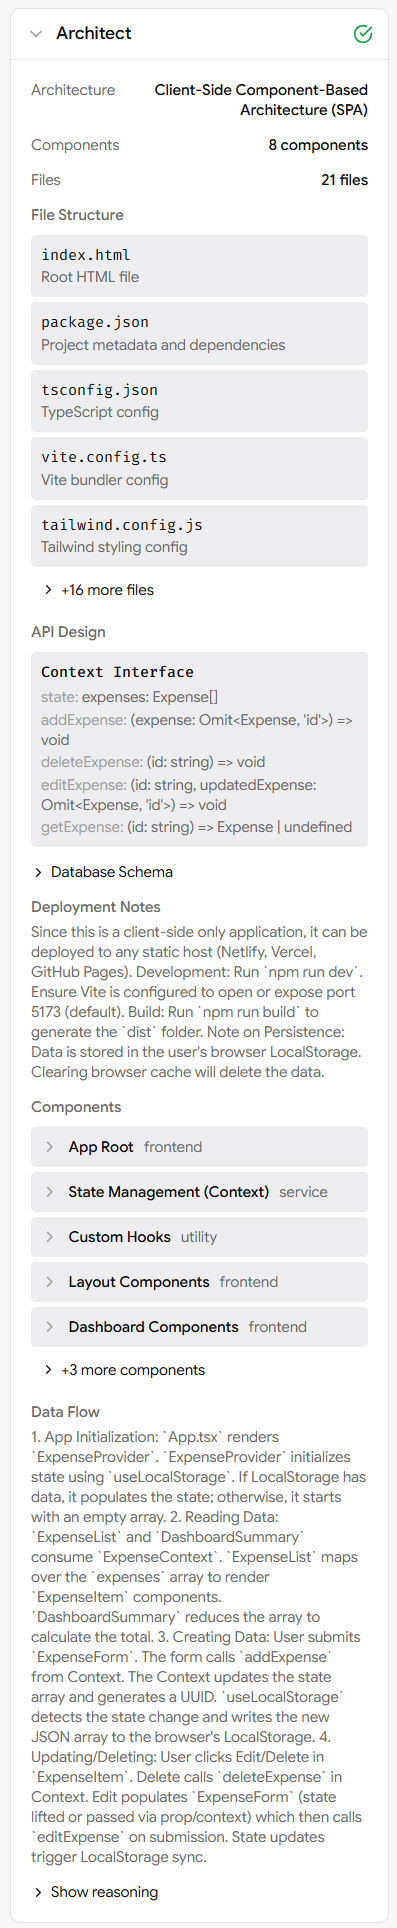
\includegraphics[height=\textheight,keepaspectratio]{images/architect_output.png}
    \label{fig:ui_architect}
\end{figure}

\vspace{1em}

\begin{figure}[H]
    \vspace*{-\intextsep}
    \centering
    \captionsetup{aboveskip=0pt,belowskip=2pt}
    \caption{MetaGPT — Engineer Agent Output}
    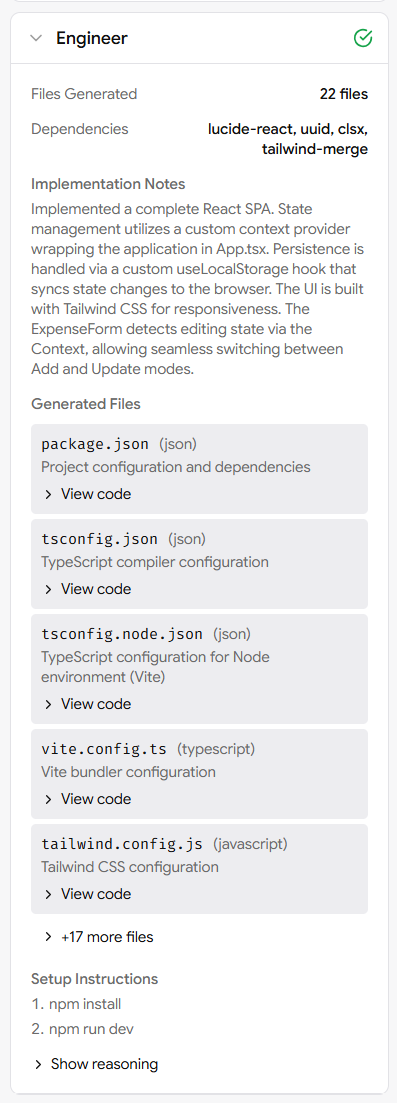
\includegraphics[height=\textheight,keepaspectratio]{images/engineer_output.png}
    \label{fig:ui_engineer}
\end{figure}

\vspace{1em}

\begin{figure}[H]
    \vspace*{-\intextsep}
    \centering
    \captionsetup{aboveskip=0pt,belowskip=2pt}
    \caption{MetaGPT — QA Agent Output}
    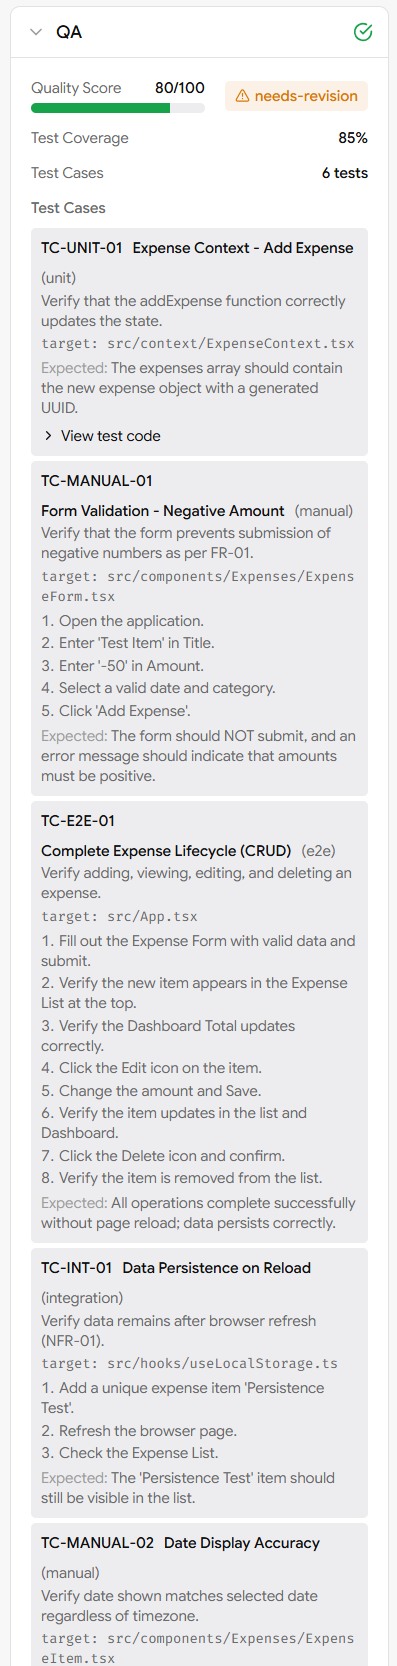
\includegraphics[height=\textheight,keepaspectratio]{images/qa_output_1.png}
    \label{fig:ui_qa}
\end{figure}

\begin{figure}[H]
    \vspace*{-\intextsep}
    \centering
    \captionsetup{aboveskip=0pt,belowskip=2pt}
    \caption{MetaGPT — QA Agent Output (continued)}
    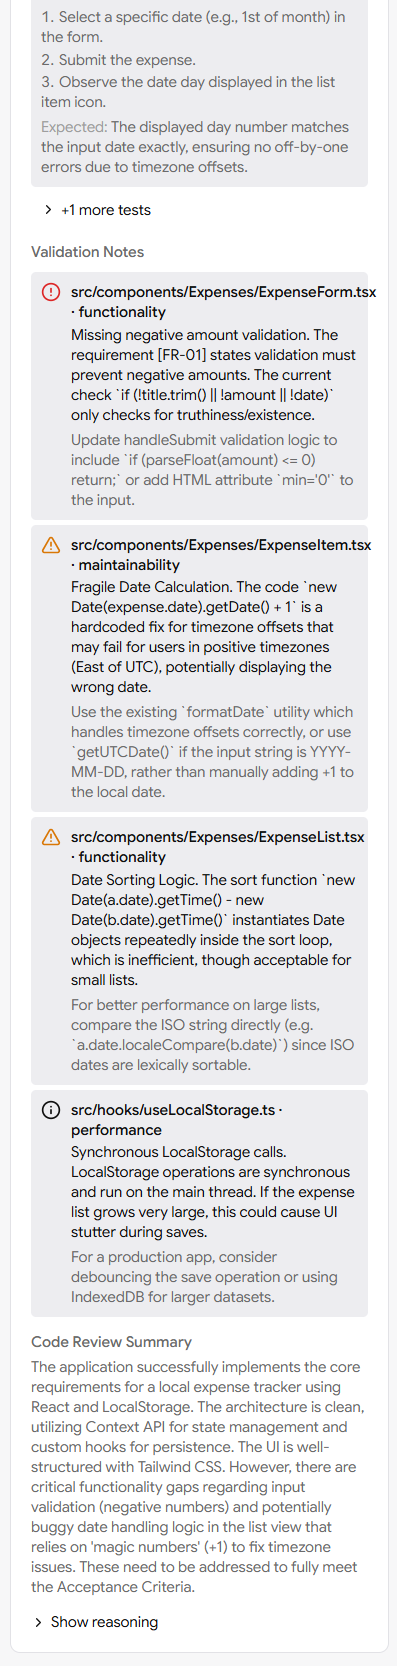
\includegraphics[height=\textheight,keepaspectratio]{images/qa_output_2.png}
    \label{fig:ui_qa_2}
\end{figure}

\vspace{1em}

\begin{figure}[H]
    \centering
    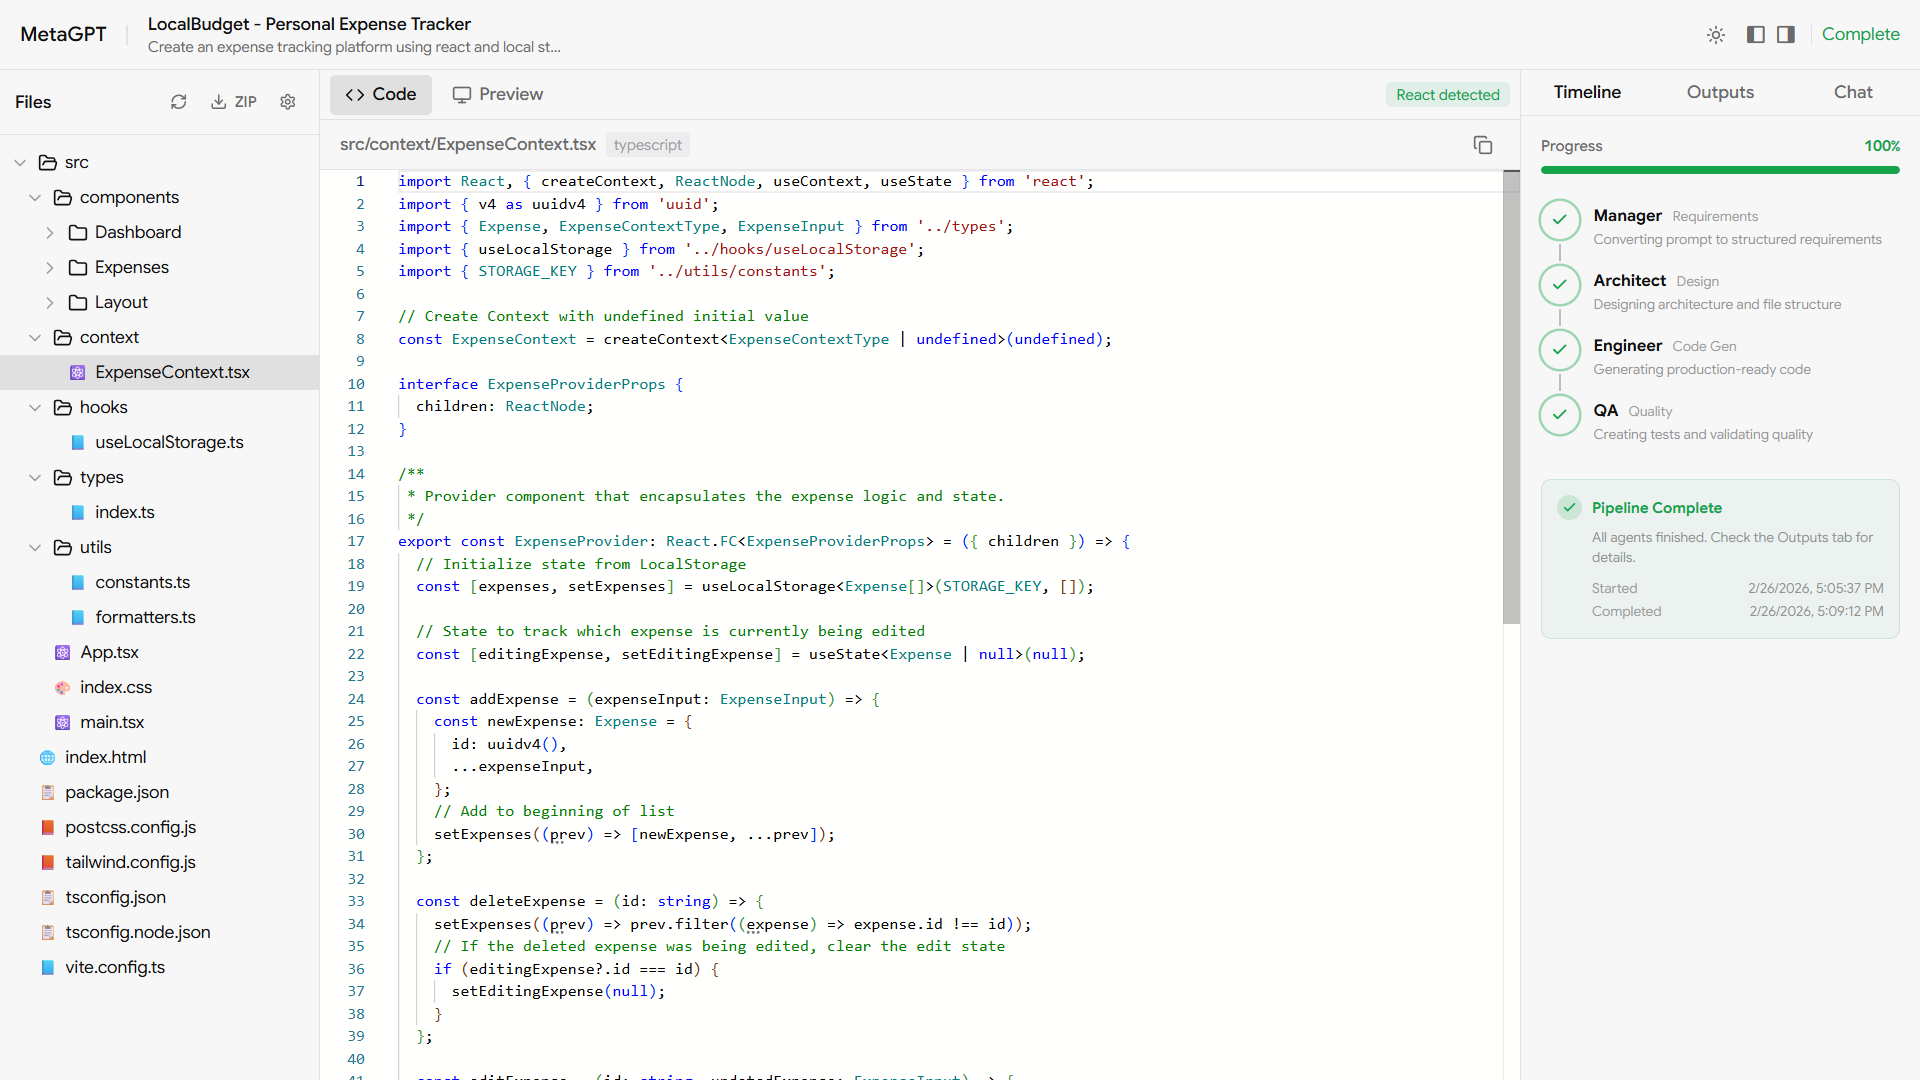
\includegraphics[width=1\textwidth]{images/code_preview.png}
    \caption{MetaGPT — Code Preview}
    \label{fig:ui_code}
\end{figure}

\vspace{1em}

\begin{figure}[H]
    \centering
    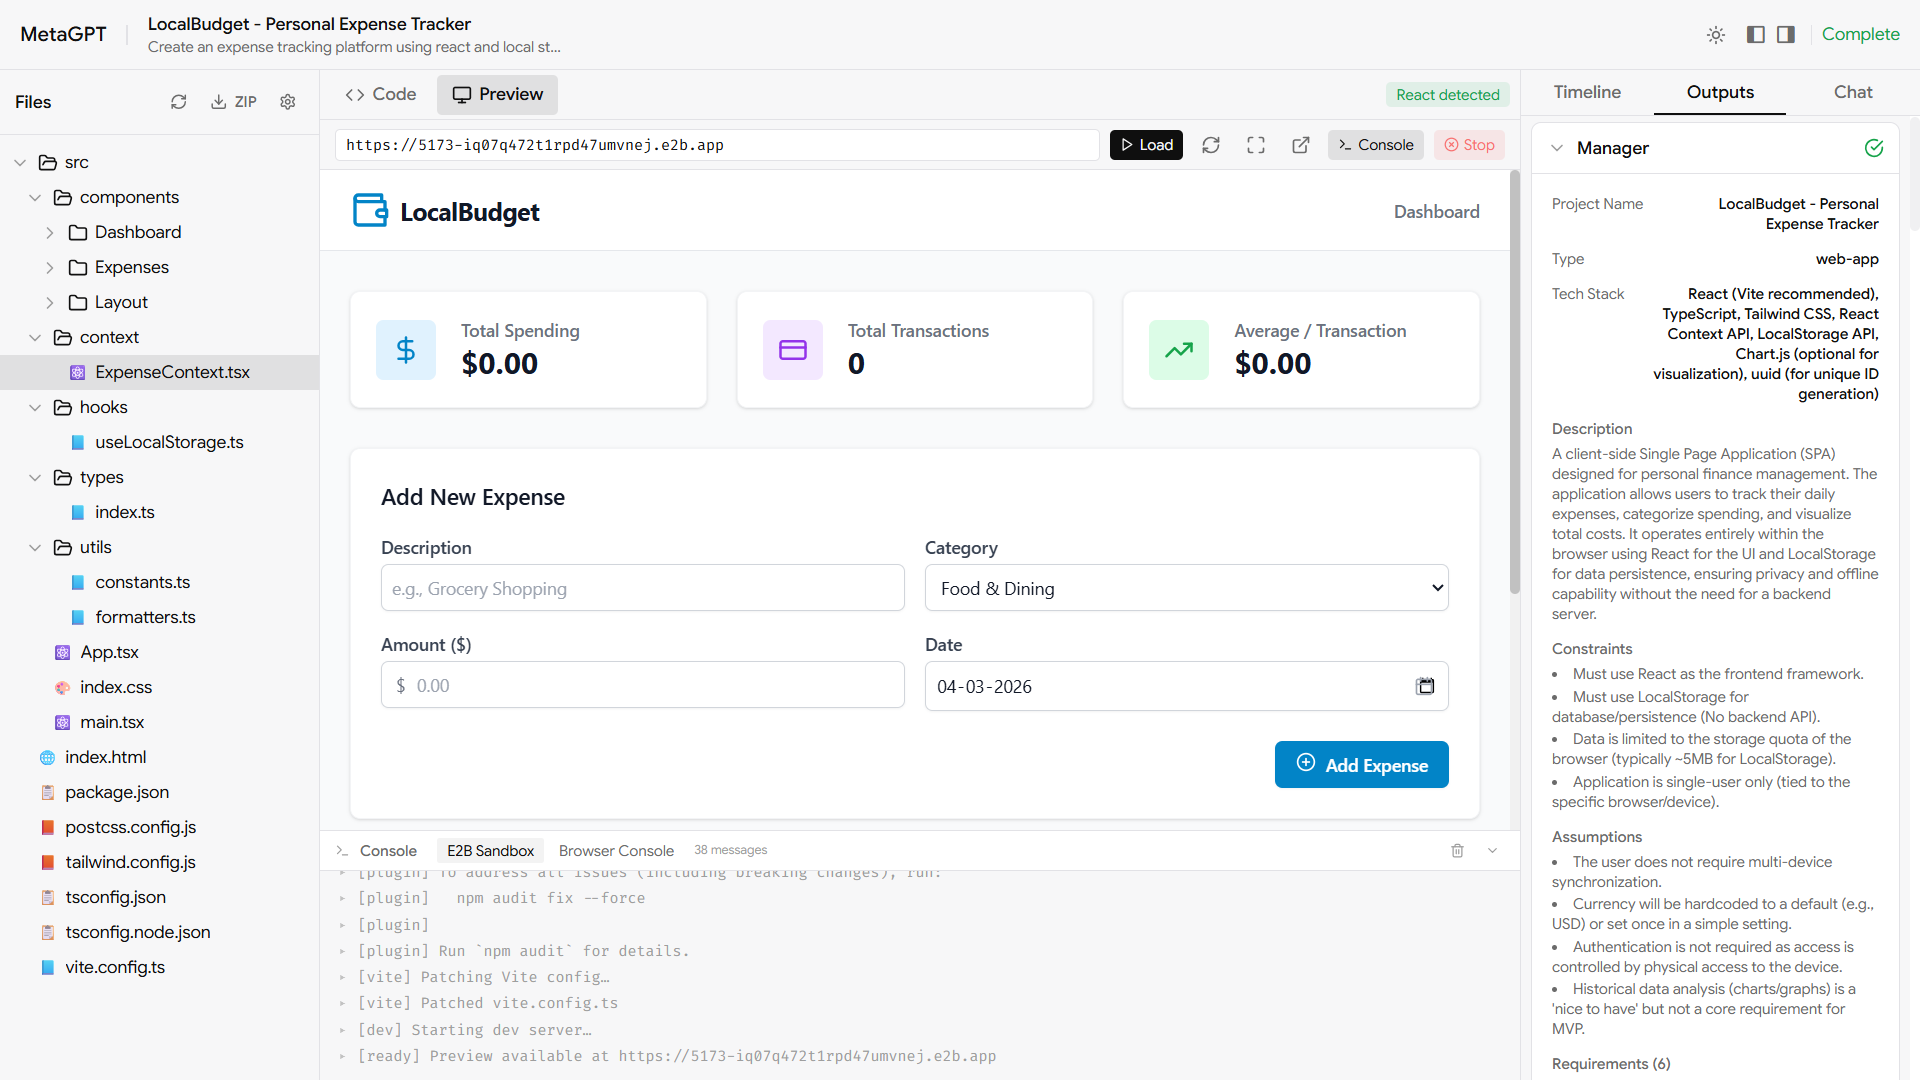
\includegraphics[width=1\textwidth]{images/sandbox_live_preview.png}
    \caption{MetaGPT — Sandbox Live Preview}
    \label{fig:ui_sandbox}
\end{figure}



\chapter{Implementation And Results}
\section{Software And Hardware Requirements}

The implementation of MetaGPT relies on a modern full-stack environment with the following software and hardware requirements:
\begin{itemize}
    \item \textbf{Hardware}: A development machine with a multi-core processor, at least 4~GB of RAM, and sufficient disk space to store generated projects. For typical experiments, a standard laptop or desktop configuration is sufficient.
    \item \textbf{Operating System}: Any operating system capable of running Python 3.11 and Node.js 18 or above (e.g., Windows, Linux, or macOS).
    \item \textbf{Backend Software}: Python 3.11+, FastAPI, LangChain, LangGraph, and supporting libraries managed using the \texttt{uv} package manager or \texttt{pip}. A valid Google API key is required to access the Gemini model.
    \item \textbf{Frontend Software}: Node.js 18+, Next.js 14, TypeScript, Tailwind CSS, and associated tooling such as ESLint and TypeScript for linting and type checking.
    \item \textbf{Tools}: Git for version control, a terminal or shell for running backend and frontend servers, and an editor or IDE for browsing code and logs.
\end{itemize}

\section{Implementation Details}

\subsection*{Module 1: Backend API Layer Implementation}

The backend is organized under \texttt{backend/\allowbreak{}app} and exposes its functionality through a FastAPI application defined in \texttt{main.py}. In this file, the FastAPI instance is created, CORS and other middleware are configured, and the top-level router from \texttt{api/\allowbreak{}router.py} is included, as shown in Listing~\ref{lst:fastapi_setup}. The router groups all versioned endpoints under the \texttt{/\allowbreak{}api/\allowbreak{}v1} prefix and delegates to modules in \texttt{api/\allowbreak{}endpoints}.

\begin{center}
\begin{minipage}{\linewidth}
\begin{lstlisting}[language=Python, caption={FastAPI application configuration and middleware setup}, label={lst:fastapi_setup}]
def create_app() -> FastAPI:
    settings = get_settings()
    app = FastAPI(
        title=settings.app_name,
        version=settings.app_version,
        lifespan=lifespan,
    )
    # Configure CORS
    app.add_middleware(
        CORSMiddleware,
        allow_origins=settings.cors_origins,
        allow_credentials=True,
        allow_methods=["*"],
        allow_headers=["*"],
    )
    # Include API routes
    app.include_router(api_router, prefix=settings.api_prefix)
    return app
\end{lstlisting}
\end{minipage}
\end{center}

Listing~\ref{lst:backend_create_project} shows a representative endpoint for creating a new project. It validates user credits, calls the pipeline service, and handles persistence.

\begin{center}
\begin{minipage}{\linewidth}
\begin{lstlisting}[language=Python, caption={FastAPI endpoint for project creation}, label={lst:backend_create_project}]
@router.post("", response_model=Project, status_code=status.HTTP_201_CREATED)
async def create_project(
    request: ProjectCreate,
    user: User = Depends(get_current_user),
) -> Project:
    if not user.has_credits():
        raise HTTPException(
            status_code=status.HTTP_403_FORBIDDEN,
            detail="You've used all your free credits. Upgrade to premium.",
        )
    service = PipelineService()
    project = await service.create_project(request.prompt, user_id=str(user.id))
    user.credits_used += 1
    await user.save()
    return project
\end{lstlisting}
\end{minipage}
\end{center}

The implementation of individual endpoints is split into focused modules:
\begin{itemize}
    \item \texttt{api/\allowbreak{}endpoints/\allowbreak{}projects.py} implements handlers for creating new projects, listing existing projects, and retrieving project metadata. It uses request/response models from \texttt{schemas/\allowbreak{}projects.py}.
    \item \texttt{api/\allowbreak{}endpoints/\allowbreak{}pipeline.py} contains endpoints to start a pipeline run (both standard and streaming) and to query pipeline status or artifacts, delegating to functions in \texttt{services/\allowbreak{}pipeline\_\allowbreak{}service.py}.
    \item \texttt{api/\allowbreak{}endpoints/\allowbreak{}files.py} provides a tree view of project files and operations to read or update file contents via the storage layer (\texttt{storage/\allowbreak{}file\_\allowbreak{}store.py}).
    \item \texttt{api/\allowbreak{}endpoints/\allowbreak{}chat.py} implements chat-based iteration endpoints that forward messages to \texttt{services/\allowbreak{}chat\_\allowbreak{}service.py}.
    \item \texttt{api/\allowbreak{}endpoints/\allowbreak{}rag.py} and \texttt{api/\allowbreak{}endpoints/\allowbreak{}sandbox.py} expose retrieval and sandbox-related operations.
\end{itemize}

Cross-cutting concerns such as authentication and authorization are implemented in \texttt{auth.py} and reused across endpoints using FastAPI dependencies. Configuration values required by the API layer are loaded from \texttt{config.py}, which reads from environment variables and provides typed settings via Pydantic.

\textbf{E2B Sandbox preview endpoints:} The sandbox endpoint module (\texttt{api/\allowbreak{}endpoints/\allowbreak{}sandbox.py}) is designed for long-running preview builds. It implements a non-blocking create flow that returns \textbf{202 Accepted} immediately and starts a background task that writes generated files, installs dependencies, and starts dev servers inside an isolated E2B sandbox. Users (via the frontend) poll the status endpoint until the sandbox becomes \texttt{ready}, at which point a public \texttt{preview\_\allowbreak{}url} is returned for embedding in an iframe.

\subsection*{Module 2: Agent Orchestration and Graph Implementation}

Agent orchestration is implemented in the \texttt{graph} and \texttt{agents} packages. The central pipeline state is defined in \texttt{graph/\allowbreak{}state.py}, where a Pydantic model captures the user prompt, derived requirements, architectural plan, generated files, and QA feedback. This state object is passed between nodes in a LangGraph graph.

The graph itself is constructed in \texttt{graph/\allowbreak{}orchestrator.py}. Here, nodes corresponding to the Manager, Architect, Engineer, and QA agents are registered, and edges are defined to specify the order of execution, as demonstrated in Listing~\ref{lst:orchestrator_graph}. Each node invokes a concrete agent class from the \texttt{agents} package:

\begin{center}
\begin{minipage}{\linewidth}
\begin{lstlisting}[language=Python, caption={LangGraph orchestrator pipeline configuration}, label={lst:orchestrator_graph}]
def _build_graph(self) -> StateGraph:
    workflow = StateGraph(PipelineState)
    # Add nodes for each agent
    workflow.add_node("manager", self._run_manager)
    workflow.add_node("architect", self._run_architect)
    workflow.add_node("engineer", self._run_engineer)
    workflow.add_node("qa", self._run_qa)

    # Define deterministic linear flow
    workflow.set_entry_point("manager")
    workflow.add_edge("manager", "architect")
    workflow.add_edge("architect", "engineer")
    workflow.add_edge("engineer", "qa")
    workflow.add_edge("qa", END)
    
    return workflow.compile()
\end{lstlisting}
\end{minipage}
\end{center}
\begin{itemize}
    \item \texttt{agents/\allowbreak{}manager.py} receives the raw prompt and produces structured requirements.
    \item \texttt{agents/\allowbreak{}architect.py} designs the system architecture and file layout based on those requirements.
    \item \texttt{agents/\allowbreak{}engineer.py} generates implementation code for the planned files. Listing~\ref{lst:engineer_prompt} illustrates how the Engineer Agent builds its LLM prompt using outputs from previous stages and SOP constraints.
    \item \texttt{agents/\allowbreak{}qa.py} inspects artifacts and produces test cases and quality feedback.
\end{itemize}

\begin{center}
\begin{minipage}{\linewidth}
\begin{lstlisting}[language=Python, caption={Engineer Agent building its prompt with context from earlier pipeline stages}, label={lst:engineer_prompt}]
def _build_prompt(self, **inputs: Any) -> str:
    architect_output: ArchitectOutput = inputs.get("architect_output")
    manager_output: ManagerOutput = inputs.get("manager_output")

    # Format SOP sections
    constraints_text = self._format_sop_section(self.sop.constraints)
    quality_text = self._format_sop_section(self.sop.quality_checklist)

    # Format architecture details
    file_structure = self._format_file_structure(architect_output)
    components = self._format_components(architect_output)
    requirements = self._format_requirements(manager_output)

    return f"""# Engineer Agent - Code Generation
## Your Role
{self.sop.role}

## Constraints
{constraints_text}

## Project: {manager_output.project_name}
{manager_output.project_description}

## File Structure:
{file_structure}

## Your Task
Implement ALL files listed in the file structure with production-ready code.
"""
\end{lstlisting}
\end{minipage}
\end{center}

All agents inherit from a base class in \texttt{agents/\allowbreak{}base.py}, which standardizes how LLM calls are made, how inputs/outputs are validated using \texttt{schemas/\allowbreak{}agents.py}, and how logging is performed. The orchestrator integrates with LangChain’s LLM abstractions provided by \texttt{llm/\allowbreak{}gemini.py}, enabling both free-form and structured-output interactions. The final orchestration API is exposed to the rest of the application through \texttt{services/\allowbreak{}pipeline\_\allowbreak{}service.py}, which provides functions to start runs, stream intermediate events, and fetch stored artifacts.

\subsection*{Module 3: Storage and Project Management Implementation}

Storage concerns are encapsulated in the \texttt{models} and \texttt{storage} packages. Domain models in \texttt{models/\allowbreak{}project.py} and \texttt{models/\allowbreak{}user.py} describe how projects and users are represented in memory, including fields such as identifiers, names, prompts, and timestamps. These models are mirrored by Pydantic schemas in \texttt{schemas/\allowbreak{}projects.py} to ensure consistency between API payloads and internal representations.

Project-level persistence is handled by \texttt{storage/\allowbreak{}project\_\allowbreak{}store.py}. This module is responsible for creating project directories under the configured \texttt{PROJECTS\_\allowbreak{}DIR}, writing metadata files if needed, and enumerating existing projects. File-level operations are implemented in \texttt{storage/\allowbreak{}file\_\allowbreak{}store.py}, which provides functions to:
\begin{itemize}
    \item Walk a project directory and build a hierarchical tree structure consumed by the frontend \texttt{FileExplorer}.
    \item Read file contents from disk and return them as text for display or further processing.
    \item Apply write operations when agents or users modify files, ensuring that paths are validated and confined to the project root.
\end{itemize}

These storage modules are consumed by both the API endpoints (for serving file trees and contents) and the agent pipeline (for writing generated code to disk). By centralizing filesystem access in a small number of modules, the system can later be extended to support alternative backends such as databases or cloud storage with minimal changes elsewhere.

\textbf{MongoDB persistence:} In our framework, project state is stored in MongoDB. The database connection is initialized in \texttt{db.py} using Motor and Beanie, and document models such as \texttt{models/\allowbreak{}project.py} and \texttt{models/\allowbreak{}user.py} are registered with Beanie. The \texttt{ProjectStore} (\texttt{storage/\allowbreak{}project\_\allowbreak{}store.py}) provides CRUD operations to create projects, update pipeline status, and persist agent outputs (Manager/Architect/Engineer/QA). Listing~\ref{lst:mongo_create} shows how a new project document is initialized and persisted. This database-backed state allows the application to restore generated files to disk when ephemeral storage is lost (e.g., after container restart), ensuring that the file explorer and subsequent operations remain consistent.

\begin{center}
\begin{minipage}{\linewidth}
\begin{lstlisting}[language=Python, caption={Creating and persisting a project document using Beanie ODM}, label={lst:mongo_create}]
async def create(self, project_id: str, prompt: str, user_id: str = "") -> Project:
    doc = ProjectDocument(
        project_id=project_id,
        user_id=user_id,
        prompt=prompt,
        state=ProjectState(
            pipeline_status=PipelineStatus(
                stage=PipelineStage.PENDING,
                progress=0,
            )
        ),
        created_at=datetime.utcnow(),
        updated_at=datetime.utcnow(),
    )
    await doc.insert()
    return self._to_project(doc)
\end{lstlisting}
\end{minipage}
\end{center}

\subsection*{Module 4: Frontend User Interface Implementation}

The frontend implementation lives in the \texttt{frontend/\allowbreak{}src} directory and is based on the Next.js App Router. Routing and layout are defined in \texttt{src/\allowbreak{}app/\allowbreak{}layout.tsx} and the various page components:
\begin{itemize}
    \item \texttt{src/\allowbreak{}app/\allowbreak{}page.tsx} implements the landing page where users can provide prompts and see high-level information about the system. A snippet handling the submission of a new project prompt is shown in Listing~\ref{lst:frontend_submit}.
    \item \texttt{src/\allowbreak{}app/\allowbreak{}projects/\allowbreak{}page.tsx} fetches the list of projects from the backend and renders them in a tabular or card-based layout.
    \item \texttt{src/\allowbreak{}app/\allowbreak{}project/\allowbreak{}[id]/\allowbreak{}page.tsx} is the main workspace, composed of panels for the file explorer, code viewer, agent outputs, execution timeline, and chat.
\end{itemize}

\begin{center}
\begin{minipage}{\linewidth}
\begin{lstlisting}[language=JavaScript, caption={Client-side form submission handler in Next.js}, label={lst:frontend_submit}]
const handleSubmit = async (e: React.FormEvent) => {
    e.preventDefault();
    if (!prompt.trim() || isLoading) return;
    if (!token) {
        router.push("/signin");
        return;
    }
    setIsLoading(true);
    try {
        const { createProject } = await import("@/lib/api");
        const project = await createProject(prompt.trim());
        router.push(`/project/${project.id}`);
    } catch (error: unknown) {
        setSubmitError("Failed to create project");
        setIsLoading(false);
    }
};
\end{lstlisting}
\end{minipage}
\end{center}

Key interactive components are implemented in \texttt{src/\allowbreak{}components}:
\begin{itemize}
    \item \texttt{FileExplorer.tsx} renders the tree returned by the files API and triggers file selection events. When only a flat list of generated files is available (e.g., streaming in real-time), it dynamically reconstructs the hierarchical folder structure as demonstrated in Listing~\ref{lst:frontend_file_tree}.
    \item \texttt{CodeViewer.tsx} uses a code editor or viewer (e.g., Monaco) to display and possibly edit source files.
    \item \texttt{AgentOutputs.tsx} subscribes to pipeline events and presents agent reasoning and outputs in a structured way.
    \item \texttt{ExecutionTimeline.tsx} visualizes the order and status of agent executions for a given run.
    \item \texttt{ChatPanel.tsx} provides a text area and message list for iterative refinement of a project as shown handling submissions in Listing~\ref{lst:chat_submit}.
\end{itemize}

\begin{center}
\begin{minipage}{\linewidth}
\begin{lstlisting}[language=JavaScript, caption={Dynamically building a file tree structure from a flat list of file paths}, label={lst:frontend_file_tree}]
function buildTreeFromFiles(files: { file_path: string }[]): FileTreeNode | null {
  if (files.length === 0) return null;

  const root: FileTreeNode = { name: "files", path: "/", type: "directory", children: [], };

  for (const file of files) {
    const parts = file.file_path.split("/").filter(Boolean);
    let current = root;

    for (let i = 0; i < parts.length; i++) {
      const part = parts[i];
      const isFile = i === parts.length - 1;
      const path = parts.slice(0, i + 1).join("/");
      let child = current.children?.find((c) => c.name === part);

      if (!child) {
        child = { name: part, path, type: isFile ? "file" : "directory", children: isFile ? [] : [], };
        current.children = current.children || [];
        current.children.push(child);
      }
      current = child;
    }
  }
  return root;
}
\end{lstlisting}
\end{minipage}
\end{center}

The module \texttt{src/\allowbreak{}lib/\allowbreak{}api.ts} centralizes HTTP calls to the backend, while \texttt{src/\allowbreak{}lib/\allowbreak{}store.ts} and related files implement client-side state management (e.g., current project, selected file, pipeline status). Tailwind CSS classes and global styles in \texttt{src/\allowbreak{}app/\allowbreak{}globals.css} are used to implement the dark theme and responsive layout.


\begin{center}
\begin{minipage}{\linewidth}
\begin{lstlisting}[language=JavaScript, caption={Chat handler supporting Server-Sent Events (SSE) and background indexing}, label={lst:chat_submit}]
const handleSubmit = async (e: React.FormEvent) => {
    e.preventDefault();
    if (!message.trim() || isLoading) return;

    const userMessage = message.trim();
    setMessage("");
    setIsLoading(true);

    try {
        const response = await sendChatMessage(
            projectId,
            userMessage,
            autoMode ? null : selectedModel,
        );

        addChatMessage({
            ...response.message,
            files_referenced: response.files_referenced,
            indexing_status: response.indexing_status,
        });

        // If indexing is pending, trigger it live
        if (response.indexing_status === "pending") {
            indexProjectFiles(projectId, response.files_modified);
        }
    } finally {
        setIsLoading(false);
    }
};
\end{lstlisting}
\end{minipage}
\end{center}


\subsection*{Module 5: LLM, SOP, and Retrieval Implementation}

The LLM, SOP, and retrieval logic is implemented in the \texttt{llm}, \texttt{sop}, and \texttt{rag} packages. The file \texttt{llm/\allowbreak{}gemini.py} exposes functions such as \texttt{get\_\allowbreak{}llm()} and \texttt{get\_\allowbreak{}llm\_\allowbreak{}with\_\allowbreak{}structured\_\allowbreak{}output(schema)} (see Listing~\ref{lst:gemini_structured}). These functions read configuration from \texttt{config.py} (e.g., model name, temperature, API key) and return LangChain \texttt{ChatModel} instances configured for MetaGPT. This ensures that all agents share a single, centrally managed LLM configuration.

\begin{center}
\begin{minipage}{\linewidth}
\begin{lstlisting}[language=Python, caption={Configuring Gemini for structured JSON output via LangChain}, label={lst:gemini_structured}]
def get_llm_with_structured_output(
    output_schema: type[T],
    temperature: float | None = None,
    max_tokens: int | None = None,
    model: str | None = None,
) -> BaseChatModel:
    base_llm = get_llm(temperature=temperature, max_tokens=max_tokens, model=model)
    return base_llm.with_structured_output(output_schema)
\end{lstlisting}
\end{minipage}
\end{center}

Agent SOPs are defined in \texttt{sop/\allowbreak{}definitions.py}. Each SOP includes fields such as role description, objectives, required inputs, expected outputs, constraints, and a quality checklist. The concrete agent classes in \texttt{agents/\allowbreak{}*.py} load these SOPs and use them to construct prompts or system messages when calling the LLM, ensuring that behavior is consistent and traceable across runs.

Retrieval-augmented generation is supported by the \texttt{rag} package:
\begin{itemize}
    \item \texttt{rag/\allowbreak{}embeddings.py} configures embedding models used to convert text into vector representations.
    \item \texttt{rag/\allowbreak{}vector\_\allowbreak{}store.py} manages storage and querying of embeddings in a vector database or in-memory index.
    \item \texttt{rag/\allowbreak{}indexer.py} defines workflows for indexing new documents, such as project files or external resources.
    \item \texttt{rag/\allowbreak{}retriever.py} implements retrieval logic that selects the most relevant chunks of text to be added as context to LLM prompts. Listing~\ref{lst:retriever_search} highlights the core similarity search function.
\end{itemize}

\begin{center}
\begin{minipage}{\linewidth}
\begin{lstlisting}[language=Python, caption={Retrieving relevant codebase chunks from the vector store}, label={lst:retriever_search}]
async def retrieve(self, project_id: str, query: str, k: int | None = None) -> list[RetrievedChunk]:
    if not self.settings.rag_enabled:
        return []

    k = k or self.settings.rag_top_k
    try:
        vector_store = get_vector_store(project_id)
        # Similarity search with scores
        results = vector_store.similarity_search_with_relevance_scores(query, k=k)

        chunks = []
        for doc, score in results:
            chunks.append(
                RetrievedChunk(
                    content=doc.page_content,
                    file_path=doc.metadata.get("file_path", "unknown"),
                    language=doc.metadata.get("language", "text"),
                    relevance_score=score,
                )
            )
        return chunks
    except Exception as e:
        logger.error(f"Retrieval error for project {project_id}: {e}")
        return []
\end{lstlisting}
\end{minipage}
\end{center}

By combining these pieces, the system can ground agent reasoning in both the current project state and external knowledge sources, improving the relevance and reliability of generated code and explanations.

\section{Testing}
\subsection{Unit Testing}

Table~\ref{tab:unit_tests} summarizes representative unit test cases for the main modules of MetaGPT. Each test case specifies the module under test, the scenario being validated, sample input, expected result, and the final status of execution.

\renewcommand{\arraystretch}{1.3}
\begingroup
\setlength{\LTleft}{-1.5cm}
\begin{longtable}{|p{3.0cm}|p{3.8cm}|p{3.8cm}|p{4.6cm}|>{\centering\arraybackslash}p{1.8cm}|}
\caption{Unit Test Cases for MetaGPT Modules}
\label{tab:unit_tests}
\\
\hline
\textbf{Module} & \textbf{Test Scenario} & \textbf{Input} & \textbf{Expected Result} & \textbf{Status} \\
\hline
\endfirsthead
\hline
\textbf{Module} & \textbf{Test Scenario} & \textbf{Input} & \textbf{Expected Result} & \textbf{Status} \\
\hline
\endhead
\hline
\endfoot
\hline
\endlastfoot
Backend API Layer & Load configuration with valid environment variables & Populated \texttt{.env} file (e.g., \texttt{GOOGLE\_\allowbreak{}API\_\allowbreak{}KEY}, \texttt{PROJECTS\_\allowbreak{}DIR}) & \texttt{Config} object created successfully with all fields set and no validation errors & Success \\
\hline
Backend API Layer & Handle missing optional configuration values & \texttt{.env} file without optional fields (e.g., no \texttt{LLM\_\allowbreak{}TEMPERATURE}) & Default values applied for missing options; application starts without raising exceptions & Success \\
\hline
Backend API Layer & Validate project creation endpoint & HTTP \texttt{POST} \texttt{/\allowbreak{}api/\allowbreak{}v1/\allowbreak{}projects} with a valid JSON body containing a prompt & Response status \texttt{201}; response body contains non-empty project ID and stored prompt & Success \\
\hline
Backend API Layer & Reject invalid project request payload & HTTP \texttt{POST} \texttt{/\allowbreak{}api/\allowbreak{}v1/\allowbreak{}projects} with missing required fields & Response status \texttt{422} (validation error); descriptive error message returned & Success \\
\hline
Backend API Layer & Fetch project list when no projects exist & HTTP \texttt{GET} \texttt{/\allowbreak{}api/\allowbreak{}v1/\allowbreak{}projects} on a clean workspace & Response status \texttt{200}; response body is an empty list & Success \\
\hline
Agent Orchestration and Graph & Initialize empty pipeline state & Call state constructor in \texttt{graph/\allowbreak{}state.py} with a sample prompt & State object created with prompt set and other fields initialized to default/empty values & Success \\
\hline
Agent Orchestration and Graph & Manager agent produces structured requirements & Invoke Manager agent with a simple prompt (mocked LLM) & Output conforms to \texttt{ManagerOutput} schema and contains non-empty requirement fields & Success \\
\hline
Agent Orchestration and Graph & Architect agent generates file plan & Provide Manager output to Architect agent (mocked LLM) & Output includes a file list with valid relative paths and descriptions & Success \\
\hline
Agent Orchestration and Graph & Graph orchestrator runs full pipeline with mocked agents & Execute orchestrator with all agents mocked to return fixed outputs & Final state contains populated requirements, architecture, code artifacts, and QA data without errors & Success \\
\hline
Agent Orchestration and Graph & Error handling in a single node & Force an exception inside one agent node & Orchestrator catches error, records it in state/logs, and terminates or retries according to policy & Success \\
\hline
Storage and Project Management & Create new project directory & Call function in \texttt{project\_\allowbreak{}store} with a new project ID & Corresponding folder created under \texttt{PROJECTS\_\allowbreak{}DIR}; path is returned and exists on disk & Success \\
\hline
Storage and Project Management & Build file tree for simple project & Populate a test project with a few files and call \texttt{file\_\allowbreak{}store} tree builder & Returned tree structure matches directory layout and contains correct file names and types & Success \\
\hline
Storage and Project Management & Read file contents safely & Request contents of a known file via \texttt{file\_\allowbreak{}store} & Function returns exact file text; attempts to escape project root are rejected & Success \\
\hline
Storage and Project Management & Update file content & Call update function with a valid file path and new code content & File on disk is overwritten with new content; subsequent read returns updated text & Success \\
\hline
Storage and Project Management & Handle non-existent file read & Request a file that does not exist in the project tree & Function raises a controlled error or returns a standardized ``not found'' response & Success \\
\hline
Frontend User Interface & Render project list page with data & Mock API client to return a list of projects and render \texttt{projects/\allowbreak{}page.tsx} & Page displays the correct number of project entries with expected titles and IDs & Success \\
\hline
Frontend User Interface & Display file contents in code viewer & Provide a selected file and mocked content to \texttt{CodeViewer.tsx} & Component renders the content in the editor area without runtime errors & Success \\
\hline
Frontend User Interface & Update selected file state on tree click & Simulate click on a file node in \texttt{FileExplorer.tsx} & Global/store state updates to mark that file as selected; dependent components receive the update & Success \\
\hline
Frontend User Interface & Show execution timeline events & Supply a sequence of mocked pipeline events to \texttt{ExecutionTimeline.tsx} & Timeline renders entries in correct order with appropriate status indicators & Success \\
\hline
Frontend User Interface & Send chat message to backend & Trigger a send action in \texttt{ChatPanel.tsx} with mocked API client & API client is called with correct project ID and message payload; UI input is cleared & Success \\
\hline
LLM, SOP, and Retrieval & Construct base LLM instance & Call \texttt{get\_\allowbreak{}llm()} from \texttt{llm/\allowbreak{}gemini.py} with valid configuration & Function returns a non-\texttt{None} LangChain model instance using configured parameters & Success \\
\hline
LLM, SOP, and Retrieval & Create structured-output LLM & Call \texttt{get\_\allowbreak{}llm\_\allowbreak{}with\_\allowbreak{}}\linebreak\texttt{structured\_\allowbreak{}output()} with a schema & Returned model enforces the specified schema and raises an error for invalid outputs in tests & Success \\
\hline
LLM, SOP, and Retrieval & Load SOP definitions & Import and access SOPs from \texttt{sop/\allowbreak{}definitions.py} & Each defined agent SOP contains non-empty role, objective, inputs, outputs, and checklist fields & Success \\
\hline
LLM, SOP, and Retrieval & Generate embeddings for sample text & Call embedding function in \texttt{rag/\allowbreak{}embeddings.py} with a short string & Function returns a numeric vector of expected dimension without errors & Success \\
\hline
LLM, SOP, and Retrieval & Retrieve nearest neighbor from vector store & Index two or more documents and query via \texttt{rag/\allowbreak{}retriever.py} & Retriever returns the most similar document to the query text according to test setup & Success \\
\hline
\end{longtable}
\endgroup

\subsection{Integration Testing}

Integration testing verifies that the various subsystems of MetaGPT---FastAPI endpoints, agent pipeline, storage, and RAG utilities---work together correctly when exercised through realistic workflows. Tables~\ref{tab:integration_api}--\ref{tab:integration_rag} summarize integration test cases for each area, using the same template as the unit testing table.

\subsubsection*{API-level Tests}
Using \texttt{pytest} and FastAPI's \texttt{TestClient}, integration tests call endpoints defined in \texttt{backend/\allowbreak{}app/\allowbreak{}api/\allowbreak{}endpoints}. Table~\ref{tab:integration_api} lists representative scenarios.

\renewcommand{\arraystretch}{1.2}
\begin{longtable}{|p{2.8cm}|p{3.4cm}|p{3.4cm}|p{4.2cm}|>{\centering\arraybackslash}p{1.6cm}|}
\caption{Integration Test Cases: API-level Tests}
\label{tab:integration_api}
\\
\hline
\textbf{Module} & \textbf{Test Scenario} & \textbf{Input} & \textbf{Expected Result} & \textbf{Status} \\
\hline
\endfirsthead
\hline
\textbf{Module} & \textbf{Test Scenario} & \textbf{Input} & \textbf{Expected Result} & \textbf{Status} \\
\hline
\endhead
\hline
\endfoot
\hline
\endlastfoot
API (Projects) & Create project and verify persistence & POST \texttt{/\allowbreak{}api/\allowbreak{}v1/\allowbreak{}projects} with \texttt{\{"prompt": "Todo app"\}} & Status 201; response has project \texttt{id}; project dir exists under \texttt{PROJECTS\_\allowbreak{}DIR} & Success \\
\hline
API (Projects) & List projects after creating one & GET \texttt{/\allowbreak{}api/\allowbreak{}v1/\allowbreak{}projects} after creating a project & Status 200; list contains at least one project with matching \texttt{id} and prompt & Success \\
\hline
API (Pipeline) & Start pipeline run and get status & POST \texttt{/\allowbreak{}api/\allowbreak{}v1/\allowbreak{}pipeline/\allowbreak{}run} with valid project \texttt{id}; then GET \texttt{/\allowbreak{}api/\allowbreak{}v1/\allowbreak{}pipeline/\allowbreak{}\{id\}/status} & Run starts; status endpoint returns run state (e.g., running/completed) and artifact keys & Success \\
\hline
API (Pipeline) & Stream pipeline events & POST \texttt{/\allowbreak{}api/\allowbreak{}v1/\allowbreak{}pipeline/\allowbreak{}stream} with prompt; consume SSE stream & Stream yields events (e.g., manager\_done, architect\_done); connection stays open until completion & Success \\
\hline
API (Files) & Get file tree for generated project & GET \texttt{/\allowbreak{}api/\allowbreak{}v1/\allowbreak{}files/\allowbreak{}\{id\}/tree} for a project with generated files & Status 200; JSON tree matches on-disk structure; nodes have \texttt{name} and \texttt{type} (file/dir) & Success \\
\hline
API (Files) & Read file content via API & GET \texttt{/\allowbreak{}api/\allowbreak{}v1/\allowbreak{}files/\allowbreak{}\{id\}/content/\{path\}} for a known file & Status 200; body contains exact file content; content-type appropriate for text & Success \\
\hline
API (Chat) & Send chat message and fetch history & POST \texttt{/\allowbreak{}api/\allowbreak{}v1/\allowbreak{}chat/\allowbreak{}\{id\}} with message; GET \texttt{/\allowbreak{}api/\allowbreak{}v1/\allowbreak{}chat/\allowbreak{}\{id\}/history} & Message stored; history returns list including the new message with correct \texttt{role} and \texttt{content} & Success \\
\hline
\end{longtable}

\subsubsection*{Pipeline Orchestration}
Tests exercise the full agent pipeline (Manager $\rightarrow$ Architect $\rightarrow$ Engineer $\rightarrow$ QA) via the LangGraph orchestrator. Table~\ref{tab:integration_pipeline} lists key scenarios.

\renewcommand{\arraystretch}{1.2}
\begin{longtable}{|p{2.8cm}|p{3.4cm}|p{3.4cm}|p{4.2cm}|>{\centering\arraybackslash}p{1.6cm}|}
\caption{Integration Test Cases: Pipeline Orchestration}
\label{tab:integration_pipeline}
\\
\hline
\textbf{Module} & \textbf{Test Scenario} & \textbf{Input} & \textbf{Expected Result} & \textbf{Status} \\
\hline
\endfirsthead
\hline
\textbf{Module} & \textbf{Test Scenario} & \textbf{Input} & \textbf{Expected Result} & \textbf{Status} \\
\hline
\endhead
\hline
\endfoot
\hline
\endlastfoot
Pipeline (Graph) & Full pipeline run with mocked LLM & Single prompt; all agents use mocked LLM returning valid structured outputs & Final state has requirements, architecture, file list, generated code, and QA output; no unhandled exceptions & Success \\
\hline
Pipeline (Graph) & State passed correctly between nodes & Inspect state after each node (Manager, Architect, Engineer, QA) & Each node receives correct input from previous node; state fields updated in order (requirements $\rightarrow$ design $\rightarrow$ code $\rightarrow$ qa) & Success \\
\hline
Pipeline (Services) & Pipeline service starts run and returns run ID & Call \texttt{pipeline\_\allowbreak{}service} start with project ID and prompt & Returns run identifier; orchestrator invoked; state persisted or streamed as configured & Success \\
\hline
Pipeline (Services) & Retrieve artifacts after run & GET artifacts for a completed pipeline run ID & Response includes manager output, architect output, engineer outputs (files), QA output in expected structure & Success \\
\hline
Pipeline (Graph) & Error in one agent does not corrupt state & Force one agent to raise; capture state/logs & Error caught; state or logs indicate which node failed; no partial writes leave inconsistent state & Success \\
\hline
\end{longtable}

\subsubsection*{Storage + API Integration}
End-to-end tests combine storage and API: create project, run pipeline (or seed files), then access via \texttt{/\allowbreak{}api/\allowbreak{}v1/\allowbreak{}files}. Table~\ref{tab:integration_storage} summarizes test cases.

\renewcommand{\arraystretch}{1.2}
\begin{longtable}{|p{2.8cm}|p{3.4cm}|p{3.4cm}|p{4.2cm}|>{\centering\arraybackslash}p{1.6cm}|}
\caption{Integration Test Cases: Storage + API Integration}
\label{tab:integration_storage}
\\
\hline
\textbf{Module} & \textbf{Test Scenario} & \textbf{Input} & \textbf{Expected Result} & \textbf{Status} \\
\hline
\endfirsthead
\hline
\textbf{Module} & \textbf{Test Scenario} & \textbf{Input} & \textbf{Expected Result} & \textbf{Status} \\
\hline
\endhead
\hline
\endfoot
\hline
\endlastfoot
Storage + API & Create project then list via API & Create project via API; add a file to project dir (simulate pipeline); GET \texttt{/\allowbreak{}api/\allowbreak{}v1/\allowbreak{}files/\allowbreak{}\{id\}/tree} & Tree includes the new file; path and name match filesystem & Success \\
\hline
Storage + API & Read file written by pipeline & Run pipeline (or seed file); GET \texttt{/\allowbreak{}api/\allowbreak{}v1/\allowbreak{}files/\allowbreak{}\{id\}/content/\allowbreak{}\{path\}} & Content returned matches content written by pipeline or test & Success \\
\hline
Storage + API & Update file via API and read back & PUT \texttt{/\allowbreak{}api/\allowbreak{}v1/\allowbreak{}files/\allowbreak{}\{id\}/content/\allowbreak{}\{path\}} with new body; GET same path & File on disk updated; GET returns new content & Success \\
\hline
Storage + API & Invalid path returns error & GET \texttt{/\allowbreak{}api/\allowbreak{}v1/\allowbreak{}files/\allowbreak{}\{id\}/content/\allowbreak{}\{path\}/../etc/\allowbreak{}passwd} or path outside project & Status 400/403/404; no content from outside project root returned & Success \\
\hline
Storage + API & Empty project returns empty tree & GET \texttt{/\allowbreak{}api/\allowbreak{}v1/\allowbreak{}files/\allowbreak{}\{id\}/tree} for newly created project with no files & Status 200; tree is empty or has only root node & Success \\
\hline
\end{longtable}

\subsubsection*{RAG Workflows}
For setups where RAG is enabled, integration tests index documents and call retrieval endpoints. Table~\ref{tab:integration_rag} lists representative cases.

\renewcommand{\arraystretch}{1.2}
\begin{longtable}{|p{2.8cm}|p{3.4cm}|p{3.4cm}|p{4.2cm}|>{\centering\arraybackslash}p{1.6cm}|}
\caption{Integration Test Cases: RAG Workflows}
\label{tab:integration_rag}
\\
\hline
\textbf{Module} & \textbf{Test Scenario} & \textbf{Input} & \textbf{Expected Result} & \textbf{Status} \\
\hline
\endfirsthead
\hline
\textbf{Module} & \textbf{Test Scenario} & \textbf{Input} & \textbf{Expected Result} & \textbf{Status} \\
\hline
\endhead
\hline
\endfoot
\hline
\endlastfoot
RAG (Indexer) & Index small document set & Call indexer with a few code snippets or file paths & Index completes; vector store contains expected number of entries; no errors & Success \\
\hline
RAG (Retriever) & Query returns relevant chunks & Index 2--3 documents; query with text similar to one document & Retriever returns chunks; top result matches or is highly similar to the queried document & Success \\
\hline
RAG + API & Retrieval endpoint returns results & GET/POST RAG endpoint with project ID and query string & Status 200; response includes retrieved snippets or IDs usable for agent context & Success \\
\hline
RAG (Embeddings) & Embeddings consistent for same text & Call embedding function twice with same string & Both calls return identical (or numerically equal) vector & Success \\
\hline
RAG (Vector store) & Add and query in same session & Add documents to vector store; run query & Query returns added documents when query text is relevant; no cross-session persistence errors & Success \\
\hline
\end{longtable}

\subsubsection*{Integration of Backend to Frontend}
Tests verify that the Next.js frontend correctly communicates with the FastAPI backend: API base URL, request/response handling, and real-time updates. Table~\ref{tab:integration_backend_frontend} lists representative scenarios.

\renewcommand{\arraystretch}{1.2}
\begin{longtable}{|p{2.8cm}|p{3.4cm}|p{3.4cm}|p{4.2cm}|>{\centering\arraybackslash}p{1.6cm}|}
\caption{Integration Test Cases: Backend to Frontend}
\label{tab:integration_backend_frontend}
\\
\hline
\textbf{Module} & \textbf{Test Scenario} & \textbf{Input} & \textbf{Expected Result} & \textbf{Status} \\
\hline
\endfirsthead
\hline
\textbf{Module} & \textbf{Test Scenario} & \textbf{Input} & \textbf{Expected Result} & \textbf{Status} \\
\hline
\endhead
\hline
\endfoot
\hline
\endlastfoot
Frontend + API & Projects list loads from backend & Open \texttt{/\allowbreak{}projects}; frontend calls GET \texttt{/\allowbreak{}api/\allowbreak{}v1/\allowbreak{}projects} & Page displays project list; data matches backend response; no CORS or network errors & Success \\
\hline
Frontend + API & Create project from UI and see in list & Submit prompt on landing/workspace; frontend POSTs to \texttt{/\allowbreak{}api/\allowbreak{}v1/\allowbreak{}projects} or pipeline & New project appears in list or workspace; project ID and prompt reflected in UI & Success \\
\hline
Frontend + API & File tree and content from backend & Select project; frontend GET \texttt{/\allowbreak{}api/\allowbreak{}v1/\allowbreak{}files/\allowbreak{}\{id\}/tree} and content endpoints & FileExplorer shows tree; CodeViewer shows file content; data matches backend storage & Success \\
\hline
Frontend + API & Pipeline run and streaming updates & Start pipeline from UI; frontend uses \texttt{/\allowbreak{}api/\allowbreak{}v1/\allowbreak{}pipeline/\allowbreak{}stream} or status poll & Execution timeline updates; agent outputs appear; run completes or shows progress without timeout & Success \\
\hline
Frontend + API & Chat message sent and history loaded & Send message in ChatPanel; frontend POST \texttt{/\allowbreak{}api/\allowbreak{}v1/\allowbreak{}chat/\allowbreak{}\{id\}}; fetch history & Message appears in UI; history GET returns same message; no duplicate or lost messages & Success \\
\hline
Frontend + API & API base URL and env configuration & Run frontend with \texttt{NEXT\_\allowbreak{}PUBLIC\_\allowbreak{}API\_\allowbreak{}URL} pointing to backend & All API calls target correct host/port; no mixed content or wrong-origin errors & Success \\
\hline
\end{longtable}

These integration tests are run alongside unit tests with:
\begin{verbatim}
cd backend
uv run pytest
\end{verbatim}
and are often marked or grouped to distinguish slower, end-to-end scenarios from fast unit tests. For the frontend, integration is validated primarily by running the application against a local backend, while automated checks such as \texttt{npm run lint} and \texttt{npm run type-check} ensure consistency between API usage and TypeScript types.

\subsection{System Testing}

System testing validates the MetaGPT project as a whole from an end-user perspective: full workflow from prompt entry to generated project, UI responsiveness, and correctness of end-to-end behaviour. Table~\ref{tab:system_tests} summarizes system-level test cases.

\renewcommand{\arraystretch}{1.2}
\begin{longtable}{|p{2.8cm}|p{3.4cm}|p{3.4cm}|p{4.2cm}|>{\centering\arraybackslash}p{1.6cm}|}
\caption{System Test Cases: Project as a Whole}
\label{tab:system_tests}
\\
\hline
\textbf{Module} & \textbf{Test Scenario} & \textbf{Input} & \textbf{Expected Result} & \textbf{Status} \\
\hline
\endfirsthead
\hline
\textbf{Module} & \textbf{Test Scenario} & \textbf{Input} & \textbf{Expected Result} & \textbf{Status} \\
\hline
\endhead
\hline
\endfoot
\hline
\endlastfoot
End-to-end & Create project from prompt to codebase & User enters prompt (e.g., ``Build a todo app with React''); runs pipeline; waits for completion & Project created; pipeline runs Manager $\rightarrow$ Architect $\rightarrow$ Engineer $\rightarrow$ QA; generated files appear in file tree; no fatal errors & Success \\
\hline
End-to-end & View and browse generated project & User opens project workspace after pipeline completion & File tree shows generated structure; selecting a file displays content in code viewer; paths and content match backend & Success \\
\hline
End-to-end & Iterate via chat and re-run pipeline & User sends chat message requesting a change; triggers follow-up run or refinement & Chat history updated; pipeline or agent responds; project state remains consistent; UI reflects changes & Success \\
\hline
End-to-end & Multiple projects in sequence & User creates Project A, then Project B; lists projects; opens each & Both projects listed; switching between projects shows correct file tree and content for each; no data mixed between projects & Success \\
\hline
End-to-end & Execution timeline reflects pipeline progress & User starts pipeline; observes timeline during run & Timeline shows agent steps (Manager, Architect, Engineer, QA) in order; status indicators update; completion state shown & Success \\
\hline
End-to-end & Landing and navigation & User opens app; navigates Landing $\rightarrow$ Projects $\rightarrow$ Project workspace & All pages load; navigation works; no blank screens or console errors; backend reachable from frontend & Success \\
\hline
End-to-end & Error handling when backend unavailable & Stop backend; perform action from frontend (e.g., load projects) & Frontend shows error or fallback; no uncaught exception; user can retry or see clear message & Success \\
\hline
End-to-end & Generated project structure is usable & Inspect generated project on disk (e.g., \texttt{PROJECTS\_\allowbreak{}DIR}) & Directory structure exists; key files (e.g., package.json, main components) present; structure aligns with Architect output & Success \\
\hline
\end{longtable}

\section{Experimental Results \& Discussion}

To evaluate MetaGPT, a series of experiments were performed using representative prompts such as ``Build a todo app with React and a REST API backend'' and ``Build a blog platform with Next.js''. For each prompt, the agent pipeline was executed end-to-end, and the resulting project structure, code quality, and test coverage were examined. The system successfully generated multi-file codebases with clear separation between frontend and backend components, along with auxiliary files such as configuration and routing modules.

Qualitative analysis showed that the SOP-driven pipeline led to more consistent architectures and clearer traceability from requirements to implementation compared to ad-hoc single-prompt generation. The execution timeline and agent output visualization also improved transparency, allowing users to understand and debug the reasoning process of each agent. Limitations observed during experimentation include sensitivity to ambiguous prompts and occasional need for manual adjustments to align generated code with specific framework versions or organizational coding standards. These observations inform the future enhancements discussed in later chapters.


\chapter{Conclusion}

This project presented the design and implementation of MetaGPT, a production-ready agentic system for transforming natural language prompts into complete software projects. By modeling the roles of a Manager, Architect, Engineer, and QA agent, and by defining clear SOPs for each, the system brings structure and traceability to LLM-based code generation. The FastAPI backend, LangGraph-based pipeline, and Next.js frontend together provide an integrated environment where users can create projects, observe pipeline execution, inspect generated artifacts, and iteratively refine outputs through chat.

Through implementation and testing, MetaGPT demonstrated that an SOP-driven, multi-agent approach can produce more consistent architectures and clearer reasoning trails than one-shot code generation tools. The system highlights the importance of modular design, explicit state management, and rich visualization when building LLM-powered developer tools. While some limitations remain, particularly around handling highly ambiguous requirements and domain-specific constraints, the work establishes a solid foundation for future research and practical deployment of agentic software engineering systems.


\chapter{Future Scope}

MetaGPT opens several avenues for future enhancement and research. One promising direction is to expand the set of supported project templates beyond React and Next.js to include mobile applications, microservices, and data engineering pipelines. This would require extending the agent SOPs and project scaffolding logic to accommodate additional frameworks, languages, and deployment targets.

Another important area is deeper integration with developer workflows, including Git-based version control, continuous integration (CI) pipelines, and deployment platforms. Features such as automatic commit generation, pull request creation, and environment provisioning would further reduce friction between generated projects and real-world engineering practices. Additionally, incorporating richer feedback loops---for example, using runtime metrics, static analysis tools, or human-in-the-loop annotations---could help the agents iteratively improve code quality and performance.

From a research perspective, MetaGPT can serve as a testbed for studying collaboration between multiple LLM agents, long-lived project memory, and adaptive SOPs that evolve over time. Exploring hybrid setups where human experts supervise or override specific agents, as well as experimenting with alternative LLM backends, are also valuable directions for future work.


% References
%%%%%%%%%%%%%%%%%%%% BIBLIOGRAPHY %%%%%%%%%%%%%%%%%%%%
\cleardoublepage
\renewcommand\bibname{References}

\addcontentsline{toc}{chapter}{References}
\begin{thebibliography}{99}

% References for MetaGPT: A Multi-Agent Collaborative Framework with RAG Enhancement

\bibitem{ref1}
H. Hong, Y. Du, J. Pan, Z. Wu, and W. Chen, "MetaGPT: Meta Programming for Multi-Agent Collaborative Framework,"
\textit{arXiv preprint arXiv:2308.00352}, 2023.

\bibitem{ref2}
M. Chen, J. Tworek, H. Jun, Q. Yuan, H. P. de Oliveira Pinto, J. Kaplan, H. Edwards, Y. Burda, N. Joseph, G. Brockman, A. Ray, R. Puri, G. Krueger, M. Petrov, H. Khlaaf, G. Sastry, P. Mishkin, S. Chan, A. Gray, N. Ryder, M. Pavlov, A. Power, L. Kaiser, M. Bavarian, C. Winter, P. Tillet, F. Such, K. Cummings, M. Plappert, F. Chantzis, E. Barnes, A. Herbert-Voss, W. Guss, A. Nichol, A. Paino, N. Tezak, J. Tang, I. Babuschkin, S. Balaji, S. Jain, A. Saunders, C. Hesse, A. N. Carr, J. Leike, J. Achiam, V. Misra, E. Morikawa, A. Radford, M. Knight, M. Brundage, M. Murati, K. Mayer, P. Welinder, B. McGrew, D. Amodei, S. McCandlish, I. Sutskever, and W. Zaremba, "Evaluating Large Language Models Trained on Code,"
\textit{arXiv preprint arXiv:2107.03374}, 2021.

\bibitem{ref3}
Y. Li, D. Choi, J. Chung, N. Kushman, J. Schrittwieser, R. Leblond, T. Eccles, J. Keeling, F. Gimeno, A. D. Lago, J. Hubert, P. Choy, C. de Masson d'Autume, I. Babuschkin, X. Chen, P. S. Huang, J. Welbl, S. Gowal, A. Cherepanov, J. Molloy, D. J. Mankowitz, E. S. G. Robson, P. Kohli, N. de Freitas, K. Kavukcuoglu, and O. Vinyals, "Competition-Level Code Generation with AlphaCode,"
\textit{Science}, vol. 378, no. 6624, pp. 1092--1097, 2022.

\bibitem{ref4}
H. Yang, S. Yue, and Y. He, "Auto-GPT for Online Decision Making: Benchmarking and Improving,"
\textit{arXiv preprint arXiv:2304.12411}, 2023.

\bibitem{ref5}
Y. Li, D. Choi, J. Chung, N. Kushman, J. Schrittwieser, R. Leblond, T. Eccles, J. Keeling, F. Gimeno, A. D. Lago, J. Hubert, P. Choy, C. de Masson d'Autume, I. Babuschkin, X. Chen, P. S. Huang, J. Welbl, S. Gowal, A. Cherepanov, J. Molloy, D. J. Mankowitz, E. S. G. Robson, P. Kohli, N. de Freitas, K. Kavukcuoglu, and O. Vinyals, "MapCoder: Multi-Agent Code Generation for Competitive Problem Solving,"
\textit{arXiv preprint arXiv:2401.14165}, 2024.

\bibitem{ref6}
S. Yao, J. Zhao, D. Yu, N. Du, I. Shafran, K. Narasimhan, and Y. Cao, "ReAct: Synergizing Reasoning and Acting in Language Models,"
\textit{arXiv preprint arXiv:2210.03629}, 2022.

\bibitem{ref7}
N. Shinn, F. Labash, and Y. Goksel, "Reflexion: An Autonomous Agent with Dynamic Memory and Self-Reflection,"
\textit{arXiv preprint arXiv:2303.11366}, 2023.

\bibitem{ref8}
T. Schick, J. Dwivedi-Yu, R. Dessì, R. Raileanu, M. Lomeli, L. Zettlemoyer, N. Cancedda, and T. Scialom, "Toolformer: Language Models Can Teach Themselves to Use Tools,"
\textit{arXiv preprint arXiv:2302.04761}, 2023.

\bibitem{ref9}
C. Qian, X. Cong, C. Yang, W. Chen, Y. Su, J. Xu, Z. Liu, and M. Sun, "ChatDev: Communicative Agents for Software Development,"
\textit{arXiv preprint arXiv:2307.07924}, 2023.

\bibitem{ref10}
P. Lewis, E. Perez, A. Piktus, F. Petroni, V. Karpukhin, N. Goyal, H. Küttler, M. Lewis, W. Yih, T. Rocktäschel, S. Riedel, and D. Kiela, "Retrieval-Augmented Generation for Knowledge-Intensive NLP Tasks,"
\textit{Advances in Neural Information Processing Systems}, vol. 33, pp. 9459--9474, 2020.

\bibitem{ref11}
A. Vaswani, N. Shazeer, N. Parmar, J. Uszkoreit, L. Jones, A. N. Gomez, Ł. Kaiser, and I. Polosukhin, "Attention is All You Need,"
\textit{Advances in Neural Information Processing Systems}, vol. 30, pp. 5998--6008, 2017.

\bibitem{ref12}
J. Wei, X. Wang, D. Schuurmans, M. Bosma, B. Ichter, F. Xia, E. Chi, Q. Le, and D. Zhou, "Chain-of-Thought Prompting Elicits Reasoning in Large Language Models,"
\textit{Advances in Neural Information Processing Systems}, vol. 35, pp. 24824--24837, 2022.

\bibitem{ref13}
LangChain, "LangChain Documentation,"
Available: \url{https://python.langchain.com/}, Accessed: Oct. 2025.

\bibitem{ref14}
LangGraph, "LangGraph Documentation,"
Available: \url{https://langchain-ai.github.io/langgraph/}, Accessed: Oct. 2025.

\bibitem{ref15}
Google, "Gemini API Documentation,"
Available: \url{https://ai.google.dev/docs}, Accessed: Oct. 2025.

\bibitem{ref16}
Tree-sitter, "Tree-sitter Documentation,"
Available: \url{https://tree-sitter.github.io/}, Accessed: Oct. 2025.

\end{thebibliography}

% Appendix
% ----------------------------------------------------------
% Appendix Main Heading (ONLY this goes to TOC)
% ----------------------------------------------------------

\clearpage
\chapter*{Appendix}
\addcontentsline{toc}{chapter}{Appendix}

\vspace{1cm}

% ----------------------------------------------------------
% Appendix I - Code Snippets
% ----------------------------------------------------------

\section*{Appendix I -- Code Snippets}

\vspace{0.5cm}

The following listings present representative source-code excerpts from the MetaGPT implementation,
covering backend API configuration, agent orchestration, storage, frontend interaction, and
retrieval-augmented generation.

\vspace{0.5cm}

\begin{center}
\begin{minipage}{\linewidth}
\begin{lstlisting}[language=Python, caption={FastAPI application configuration and middleware setup}, label={lst:fastapi_setup}]
def create_app() -> FastAPI:
    settings = get_settings()
    app = FastAPI(
        title=settings.app_name,
        version=settings.app_version,
        lifespan=lifespan,
    )
    # Configure CORS
    app.add_middleware(
        CORSMiddleware,
        allow_origins=settings.cors_origins,
        allow_credentials=True,
        allow_methods=["*"],
        allow_headers=["*"],
    )
    # Include API routes
    app.include_router(api_router, prefix=settings.api_prefix)
    return app
\end{lstlisting}
\end{minipage}
\end{center}

\vspace{0.5cm}

\begin{center}
\begin{minipage}{\linewidth}
\begin{lstlisting}[language=Python, caption={FastAPI endpoint for project creation}, label={lst:backend_create_project}]
@router.post("", response_model=Project, status_code=status.HTTP_201_CREATED)
async def create_project(
    request: ProjectCreate,
    user: User = Depends(get_current_user),
) -> Project:
    if not user.has_credits():
        raise HTTPException(
            status_code=status.HTTP_403_FORBIDDEN,
            detail="You've used all your free credits. Upgrade to premium.",
        )
    service = PipelineService()
    project = await service.create_project(request.prompt, user_id=str(user.id))
    user.credits_used += 1
    await user.save()
    return project
\end{lstlisting}
\end{minipage}
\end{center}

\vspace{0.5cm}

\begin{center}
\begin{minipage}{\linewidth}
\begin{lstlisting}[language=Python, caption={LangGraph orchestrator pipeline configuration}, label={lst:orchestrator_graph}]
def _build_graph(self) -> StateGraph:
    workflow = StateGraph(PipelineState)
    # Add nodes for each agent
    workflow.add_node("manager", self._run_manager)
    workflow.add_node("architect", self._run_architect)
    workflow.add_node("engineer", self._run_engineer)
    workflow.add_node("qa", self._run_qa)

    # Define deterministic linear flow
    workflow.set_entry_point("manager")
    workflow.add_edge("manager", "architect")
    workflow.add_edge("architect", "engineer")
    workflow.add_edge("engineer", "qa")
    workflow.add_edge("qa", END)
    
    return workflow.compile()
\end{lstlisting}
\end{minipage}
\end{center}

\vspace{0.5cm}

\begin{center}
\begin{minipage}{\linewidth}
\begin{lstlisting}[language=Python, caption={Engineer Agent building its prompt with context from earlier pipeline stages}, label={lst:engineer_prompt}]
def _build_prompt(self, **inputs: Any) -> str:
    architect_output: ArchitectOutput = inputs.get("architect_output")
    manager_output: ManagerOutput = inputs.get("manager_output")

    # Format SOP sections
    constraints_text = self._format_sop_section(self.sop.constraints)
    quality_text = self._format_sop_section(self.sop.quality_checklist)

    # Format architecture details
    file_structure = self._format_file_structure(architect_output)
    components = self._format_components(architect_output)
    requirements = self._format_requirements(manager_output)

    return f"""# Engineer Agent - Code Generation
## Your Role
{self.sop.role}

## Constraints
{constraints_text}

## Project: {manager_output.project_name}
{manager_output.project_description}

## File Structure:
{file_structure}

## Your Task
Implement ALL files listed in the file structure with production-ready code.
"""
\end{lstlisting}
\end{minipage}
\end{center}

\vspace{0.5cm}

\begin{center}
\begin{minipage}{\linewidth}
\begin{lstlisting}[language=Python, caption={Creating and persisting a project document using Beanie ODM}, label={lst:mongo_create}]
async def create(self, project_id: str, prompt: str, user_id: str = "") -> Project:
    doc = ProjectDocument(
        project_id=project_id,
        user_id=user_id,
        prompt=prompt,
        state=ProjectState(
            pipeline_status=PipelineStatus(
                stage=PipelineStage.PENDING,
                progress=0,
            )
        ),
        created_at=datetime.utcnow(),
        updated_at=datetime.utcnow(),
    )
    await doc.insert()
    return self._to_project(doc)
\end{lstlisting}
\end{minipage}
\end{center}

\vspace{0.5cm}

\begin{center}
\begin{minipage}{\linewidth}
\begin{lstlisting}[language=JavaScript, caption={Client-side form submission handler in Next.js}, label={lst:frontend_submit}]
const handleSubmit = async (e: React.FormEvent) => {
    e.preventDefault();
    if (!prompt.trim() || isLoading) return;
    if (!token) {
        router.push("/signin");
        return;
    }
    setIsLoading(true);
    try {
        const { createProject } = await import("@/lib/api");
        const project = await createProject(prompt.trim());
        router.push(`/project/${project.id}`);
    } catch (error: unknown) {
        setSubmitError("Failed to create project");
        setIsLoading(false);
    }
};
\end{lstlisting}
\end{minipage}
\end{center}

\vspace{0.5cm}

\begin{center}
\begin{minipage}{\linewidth}
\begin{lstlisting}[language=JavaScript, caption={Dynamically building a file tree structure from a flat list of file paths}, label={lst:frontend_file_tree}]
function buildTreeFromFiles(files: { file_path: string }[]): FileTreeNode | null {
  if (files.length === 0) return null;

  const root: FileTreeNode = { name: "files", path: "/", type: "directory", children: [], };

  for (const file of files) {
    const parts = file.file_path.split("/").filter(Boolean);
    let current = root;

    for (let i = 0; i < parts.length; i++) {
      const part = parts[i];
      const isFile = i === parts.length - 1;
      const path = parts.slice(0, i + 1).join("/");
      let child = current.children?.find((c) => c.name === part);

      if (!child) {
        child = { name: part, path, type: isFile ? "file" : "directory", children: isFile ? [] : [], };
        current.children = current.children || [];
        current.children.push(child);
      }
      current = child;
    }
  }
  return root;
}
\end{lstlisting}
\end{minipage}
\end{center}

\vspace{0.5cm}

\begin{center}
\begin{minipage}{\linewidth}
\begin{lstlisting}[language=JavaScript, caption={Chat handler supporting Server-Sent Events (SSE) and background indexing}, label={lst:chat_submit}]
const handleSubmit = async (e: React.FormEvent) => {
    e.preventDefault();
    if (!message.trim() || isLoading) return;

    const userMessage = message.trim();
    setMessage("");
    setIsLoading(true);

    try {
        const response = await sendChatMessage(
            projectId,
            userMessage,
            autoMode ? null : selectedModel,
        );

        addChatMessage({
            ...response.message,
            files_referenced: response.files_referenced,
            indexing_status: response.indexing_status,
        });

        // If indexing is pending, trigger it live
        if (response.indexing_status === "pending") {
            indexProjectFiles(projectId, response.files_modified);
        }
    } finally {
        setIsLoading(false);
    }
};
\end{lstlisting}
\end{minipage}
\end{center}

\vspace{0.5cm}

\begin{center}
\begin{minipage}{\linewidth}
\begin{lstlisting}[language=Python, caption={Configuring Gemini for structured JSON output via LangChain}, label={lst:gemini_structured}]
def get_llm_with_structured_output(
    output_schema: type[T],
    temperature: float | None = None,
    max_tokens: int | None = None,
    model: str | None = None,
) -> BaseChatModel:
    base_llm = get_llm(temperature=temperature, max_tokens=max_tokens, model=model)
    return base_llm.with_structured_output(output_schema)
\end{lstlisting}
\end{minipage}
\end{center}

\vspace{0.5cm}

\begin{center}
\begin{minipage}{\linewidth}
\begin{lstlisting}[language=Python, caption={Retrieving relevant codebase chunks from the vector store}, label={lst:retriever_search}]
async def retrieve(self, project_id: str, query: str, k: int | None = None) -> list[RetrievedChunk]:
    if not self.settings.rag_enabled:
        return []

    k = k or self.settings.rag_top_k
    try:
        vector_store = get_vector_store(project_id)
        # Similarity search with scores
        results = vector_store.similarity_search_with_relevance_scores(query, k=k)

        chunks = []
        for doc, score in results:
            chunks.append(
                RetrievedChunk(
                    content=doc.page_content,
                    file_path=doc.metadata.get("file_path", "unknown"),
                    language=doc.metadata.get("language", "text"),
                    relevance_score=score,
                )
            )
        return chunks
    except Exception as e:
        logger.error(f"Retrieval error for project {project_id}: {e}")
        return []
\end{lstlisting}
\end{minipage}
\end{center}

\vspace{0.5cm}

\begin{center}
\begin{minipage}{\linewidth}
\begin{lstlisting}[language=Python, caption={BaseAgent: core LLM invocation loop with structured output and execution statistics}, label={lst:base_agent_execute}]
async def execute(self, **inputs: Any) -> T:
    start_time = time.time()

    # Build the prompt from SOP template
    prompt = self._build_prompt(**inputs)

    # Get LLM configured for structured output
    llm = get_llm_with_structured_output(self.output_schema)

    # Create messages
    messages = [
        SystemMessage(content=self.sop.role),
        HumanMessage(content=prompt),
    ]

    # Execute and get structured response
    try:
        result = await llm.ainvoke(messages)

        self._execution_stats = {
            "execution_time_ms": int((time.time() - start_time) * 1000),
            "status": "success",
            "agent_name": self.name,
        }
        return result

    except Exception as e:
        self._execution_stats = {
            "execution_time_ms": int((time.time() - start_time) * 1000),
            "status": "error",
            "error": str(e),
            "agent_name": self.name,
        }
        raise
\end{lstlisting}
\end{minipage}
\end{center}

\vspace{0.5cm}

\begin{center}
\begin{minipage}{\linewidth}
\begin{lstlisting}[language=Python, caption={LangGraph PipelineState TypedDict and initial state factory}, label={lst:pipeline_state}]
class PipelineState(TypedDict, total=False):
    """State that flows through the LangGraph pipeline."""

    # Input
    project_id: str
    user_prompt: str
    context: str

    # Agent outputs
    manager_output:  ManagerOutput  | None
    architect_output: ArchitectOutput | None
    engineer_output:  EngineerOutput  | None
    qa_output:        QAOutput        | None

    # Pipeline tracking
    current_stage: Literal[
        "pending", "manager", "architect", "engineer", "qa", "completed", "error"
    ]
    progress: float
    error: str | None
    execution_log: list[dict[str, Any]]


def create_initial_state(project_id: str, user_prompt: str, context: str = "") -> PipelineState:
    """Create initial pipeline state from user input."""
    return PipelineState(
        project_id=project_id,
        user_prompt=user_prompt,
        context=context,
        manager_output=None,
        architect_output=None,
        engineer_output=None,
        qa_output=None,
        current_stage="pending",
        progress=0.0,
        error=None,
        started_at=datetime.utcnow().isoformat(),
        completed_at=None,
        execution_log=[],
    )
\end{lstlisting}
\end{minipage}
\end{center}

\vspace{0.5cm}

\begin{center}
\begin{minipage}{\linewidth}
\begin{lstlisting}[language=Python, caption={ManagerAgent: SOP-driven prompt construction for requirements extraction}, label={lst:manager_prompt}]
class ManagerAgent(BaseAgent[ManagerOutput]):
    """Manager Agent - Converts user prompts to structured requirements."""

    def __init__(self):
        super().__init__(sop=MANAGER_SOP, output_schema=ManagerOutput)

    @property
    def name(self) -> str:
        return "ManagerAgent"

    def _build_prompt(self, **inputs: Any) -> str:
        user_prompt = inputs.get("user_prompt", "")
        context = inputs.get("context", "No additional context provided.")

        constraints_text = self._format_sop_section(self.sop.constraints)
        quality_text = self._format_sop_section(self.sop.quality_checklist)

        return self.sop.prompt_template.format(
            role=self.sop.role,
            objective=self.sop.objective,
            constraints=constraints_text,
            quality_checklist=quality_text,
            user_prompt=user_prompt,
            context=context,
        )


async def run_manager_agent(user_prompt: str, context: str = "") -> ManagerOutput:
    """Convenience function to run the Manager Agent."""
    agent = ManagerAgent()
    return await agent.execute(user_prompt=user_prompt, context=context)
\end{lstlisting}
\end{minipage}
\end{center}

\vspace{0.5cm}

\begin{center}
\begin{minipage}{\linewidth}
\begin{lstlisting}[language=Python, caption={JWT authentication: token creation and FastAPI dependency for current user}, label={lst:jwt_auth}]
def create_access_token(user_id: str, email: str) -> str:
    """Create a JWT access token for a user."""
    settings = get_settings()
    expire = datetime.utcnow() + timedelta(hours=settings.jwt_expiration_hours)
    payload = {"sub": user_id, "email": email, "exp": expire}
    return jwt.encode(payload, settings.jwt_secret, algorithm=settings.jwt_algorithm)


async def get_current_user(
    credentials: Annotated[HTTPAuthorizationCredentials, Depends(security)],
) -> User:
    """FastAPI dependency: validates JWT and returns the User from MongoDB."""
    settings = get_settings()
    token = credentials.credentials

    credentials_exception = HTTPException(
        status_code=status.HTTP_401_UNAUTHORIZED,
        detail="Invalid or expired token",
        headers={"WWW-Authenticate": "Bearer"},
    )

    try:
        payload = jwt.decode(token, settings.jwt_secret, algorithms=[settings.jwt_algorithm])
        user_id: str | None = payload.get("sub")
        if user_id is None:
            raise credentials_exception
    except JWTError:
        raise credentials_exception

    try:
        user = await User.get(PydanticObjectId(user_id))
    except Exception:
        raise credentials_exception

    if user is None:
        raise credentials_exception

    return user
\end{lstlisting}
\end{minipage}
\end{center}

\vspace{0.5cm}

\begin{center}
\begin{minipage}{\linewidth}
\begin{lstlisting}[language=Python, caption={CodebaseIndexer: language-aware file chunking and vector store ingestion}, label={lst:indexer_project}]
def _get_splitter(self, file_path: str) -> RecursiveCharacterTextSplitter:
    """Get a language-aware text splitter for the file type."""
    ext = Path(file_path).suffix.lower()
    language = _LANGUAGE_MAP.get(ext)

    if language:
        return RecursiveCharacterTextSplitter.from_language(
            language=language,
            chunk_size=self.settings.rag_chunk_size,
            chunk_overlap=self.settings.rag_chunk_overlap,
        )
    return RecursiveCharacterTextSplitter(
        chunk_size=self.settings.rag_chunk_size,
        chunk_overlap=self.settings.rag_chunk_overlap,
        separators=["\n\n", "\n", " ", ""],
    )


async def index_project(self, project_id: str) -> dict:
    """Index all files in a project into the vector store."""
    file_paths = await self.file_store.list_files(project_id)
    documents = []

    for file_path in file_paths:
        if self._should_skip(file_path):
            continue
        file_data = await self.file_store.read_file(project_id, file_path)
        if not file_data or not file_data.content.strip():
            continue

        splitter = self._get_splitter(file_path)
        for i, chunk in enumerate(splitter.split_text(file_data.content)):
            documents.append(Document(
                page_content=chunk,
                metadata={
                    "file_path": file_path,
                    "language": file_data.language,
                    "chunk_index": i,
                    "project_id": project_id,
                    "indexed_at": datetime.utcnow().isoformat(),
                },
            ))

    vector_store = get_vector_store(project_id)
    vector_store.add_documents(documents)
    return {"files_indexed": len(set(d.metadata["file_path"] for d in documents)),
            "chunks_created": len(documents)}
\end{lstlisting}
\end{minipage}
\end{center}

\vspace{0.5cm}

\begin{center}
\begin{minipage}{\linewidth}
\begin{lstlisting}[language=Python, caption={ChatService: RAG-driven file selection and single-LLM-call edit flow}, label={lst:chat_service}]
async def process_message(self, project_id: str, request: ChatRequest) -> ChatResponse:
    """
    Process a chat message to produce targeted file edits.
    Flow: RAG retrieval -> read file contents -> single LLM call -> write changes.
    """
    all_file_paths = await self.file_store.list_files(project_id)

    # Build file context: all files for small projects, RAG-selected for large ones
    if len(all_file_paths) <= 30:
        file_context = await self._read_all_files(project_id, all_file_paths)
    elif self.settings.rag_enabled:
        relevant = await self.retriever.retrieve_files(project_id, request.message, k=15)
        file_context = "\n\n".join(
            f"### {f['file_path']} ({f['language']})\n```{f['language']}\n{f['content']}\n```"
            for f in relevant
        )
    else:
        file_context = await self._read_all_files(project_id, all_file_paths)

    # Single LLM call for targeted edits
    llm_result = await self._call_llm(request.message, file_context, all_file_paths)

    # Write modified files to disk and update MongoDB
    files_modified = []
    for file_data in llm_result.get("files", []):
        spec = GeneratedFileSpec(**file_data)
        await self.file_store.write_file(project_id, spec)
        files_modified.append(spec.file_path)

    if files_modified:
        await self._update_project_state(project_id, files_modified)

    return ChatResponse(
        message=ChatMessage(role="assistant",
                            content=llm_result.get("summary", "Done.")),
        files_modified=files_modified,
        indexing_status="pending" if files_modified and self.settings.rag_enabled else None,
    )
\end{lstlisting}
\end{minipage}
\end{center}

\vspace{0.5cm}

\begin{center}
\begin{minipage}{\linewidth}
\begin{lstlisting}[language=Python, caption={MongoDB initialisation with Motor and Beanie ODM}, label={lst:db_init}]
async def init_db() -> None:
    """Initialize the MongoDB connection and Beanie ODM."""
    from app.models.user import User
    from app.models.project import ProjectDocument

    settings = get_settings()
    client = AsyncIOMotorClient(settings.mongodb_uri)
    db = client[settings.mongodb_db]

    await init_beanie(
        database=db,
        document_models=[User, ProjectDocument],
    )
\end{lstlisting}
\end{minipage}
\end{center}


\end{document}